\section{Soft drop method in future collider performance}
In this section, we use the specific method about the soft-drop to study the performance of the detector in the different cell sizes.  In the Figure , , , , are the distribution of the signal and background. 
\subsection{Analysis method}
In this analysis, We fix the central at the median in signal distribution, and we use the different width to open the window to draw ROC curves.
\subsection{The conclusion of the results}

 
%50bins
\begin{figure}
\begin{center}
   \subfigure[5TeV at 20$\times$20(cm$\times$cm) in cluster] {
   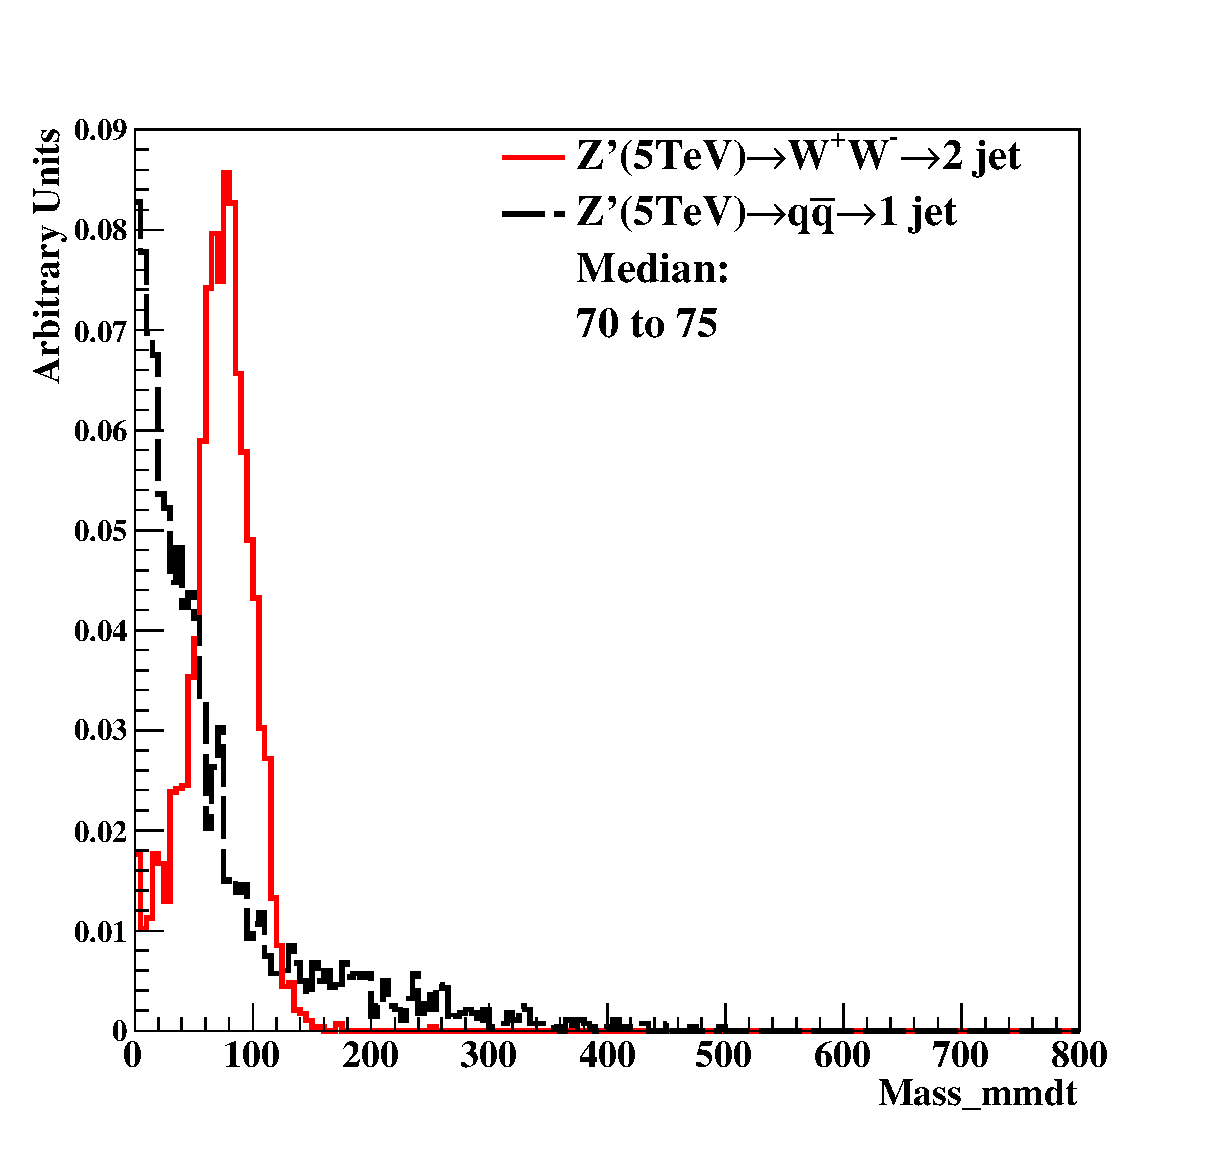
\includegraphics[width=0.22\textwidth]{figs/Dis_cluster_010_mass_mmdt_5tev_04_no_UOF.eps}
   }
      \subfigure[10TeV at 20$\times$20(cm$\times$cm) in cluster] {
   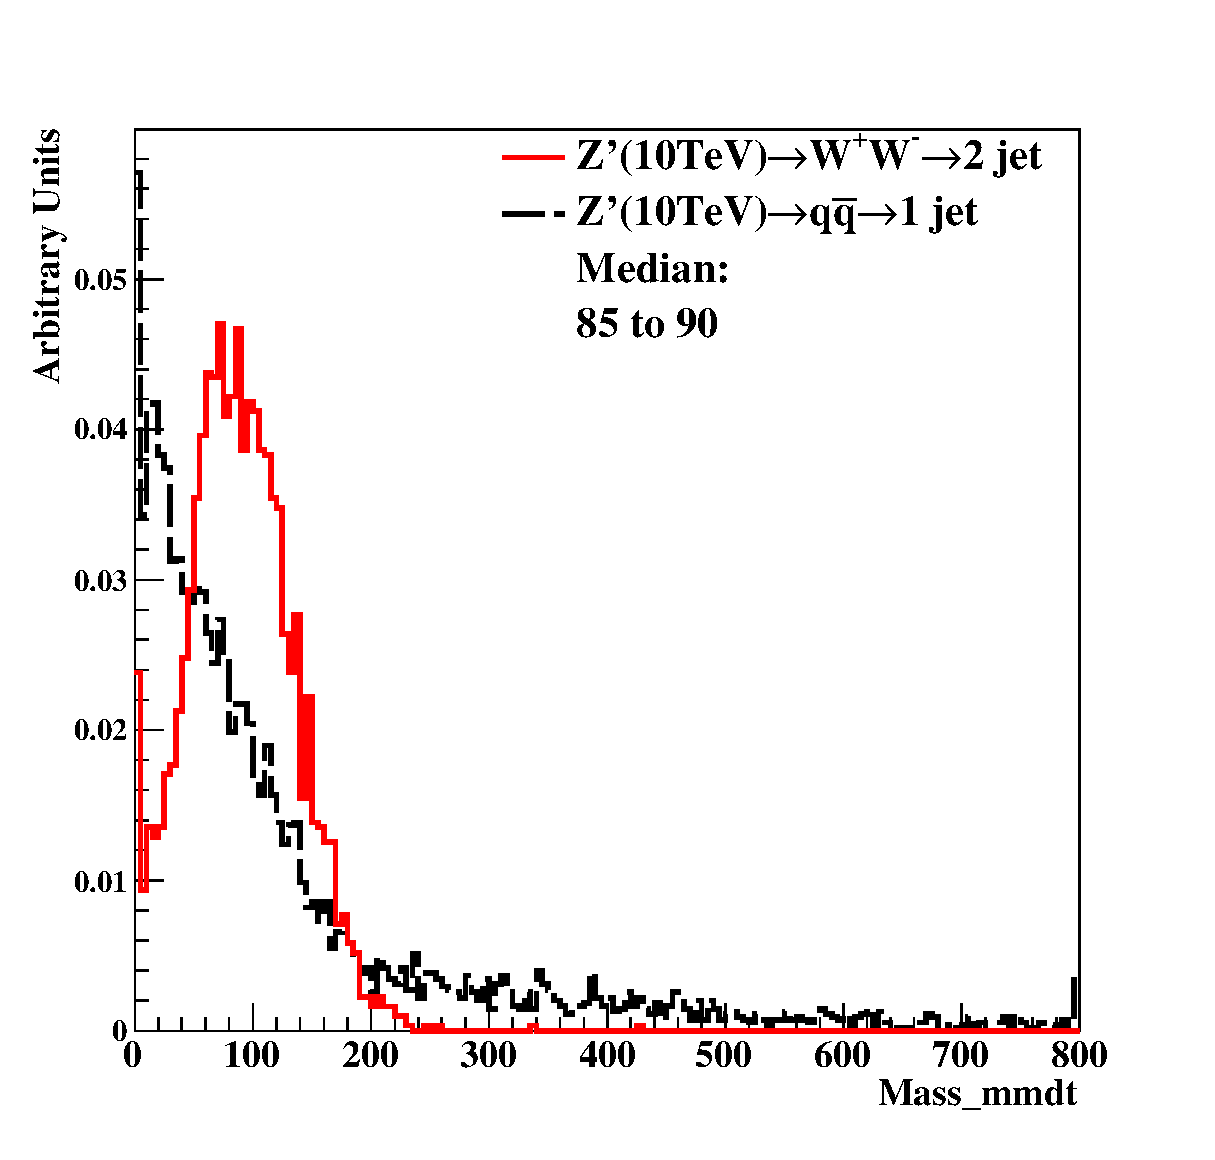
\includegraphics[width=0.22\textwidth]{figs/Dis_cluster_010_mass_mmdt_10tev_04_no_UOF.eps}
   }
   \subfigure[20TeV at 20$\times$20(cm$\times$cm) in cluster] {
   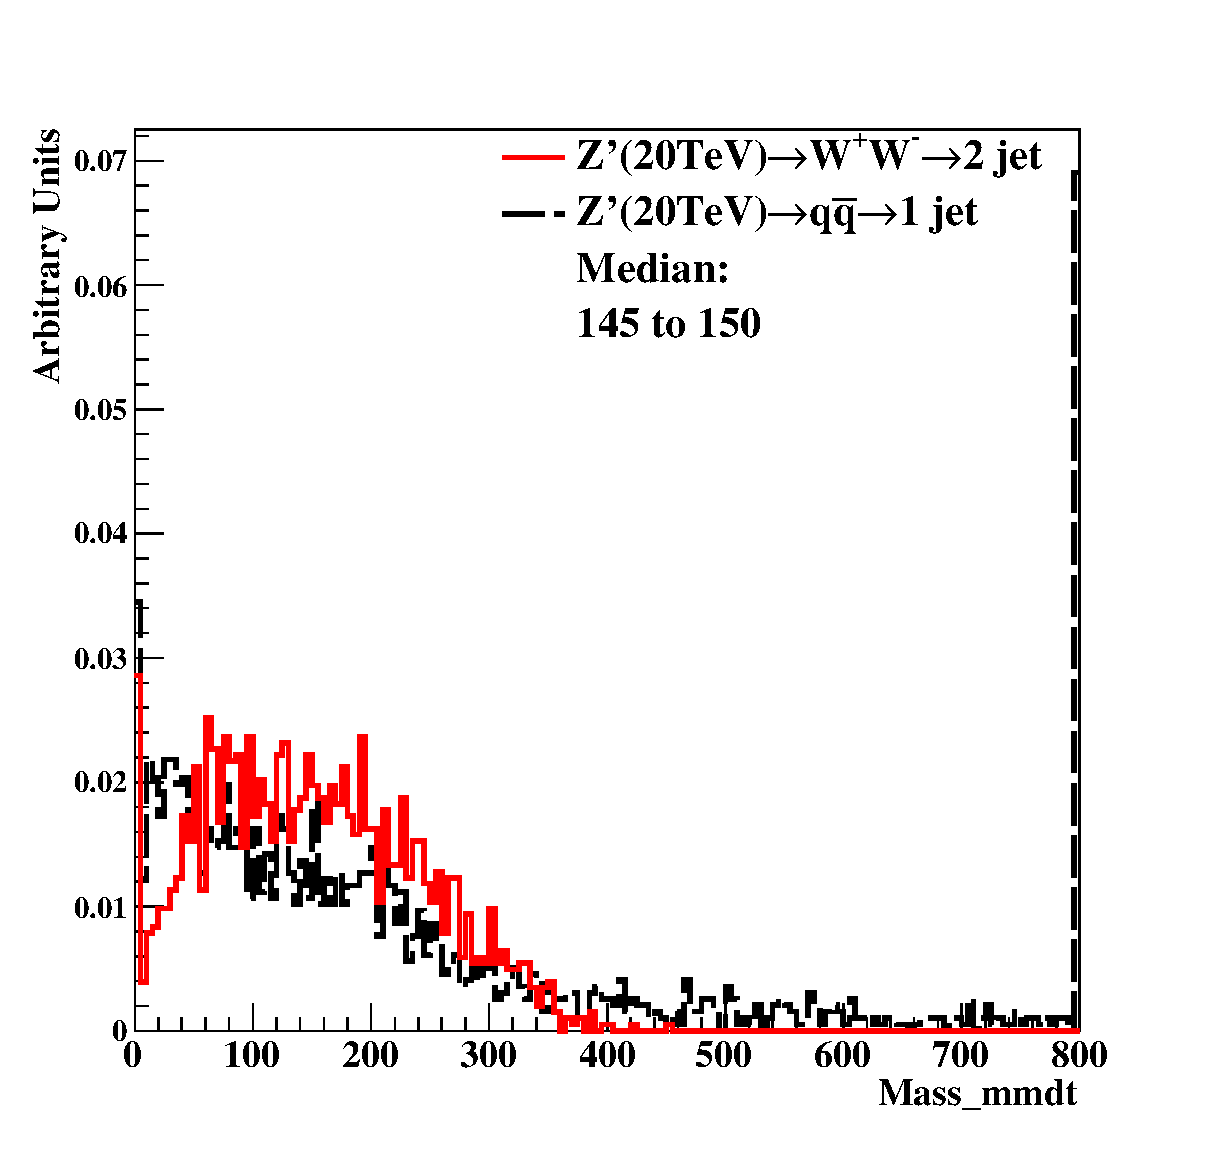
\includegraphics[width=0.22\textwidth]{figs/Dis_cluster_010_mass_mmdt_20tev_04_no_UOF.eps}
   }
    \subfigure[40TeV at 20$\times$20(cm$\times$cm) in cluster] {
   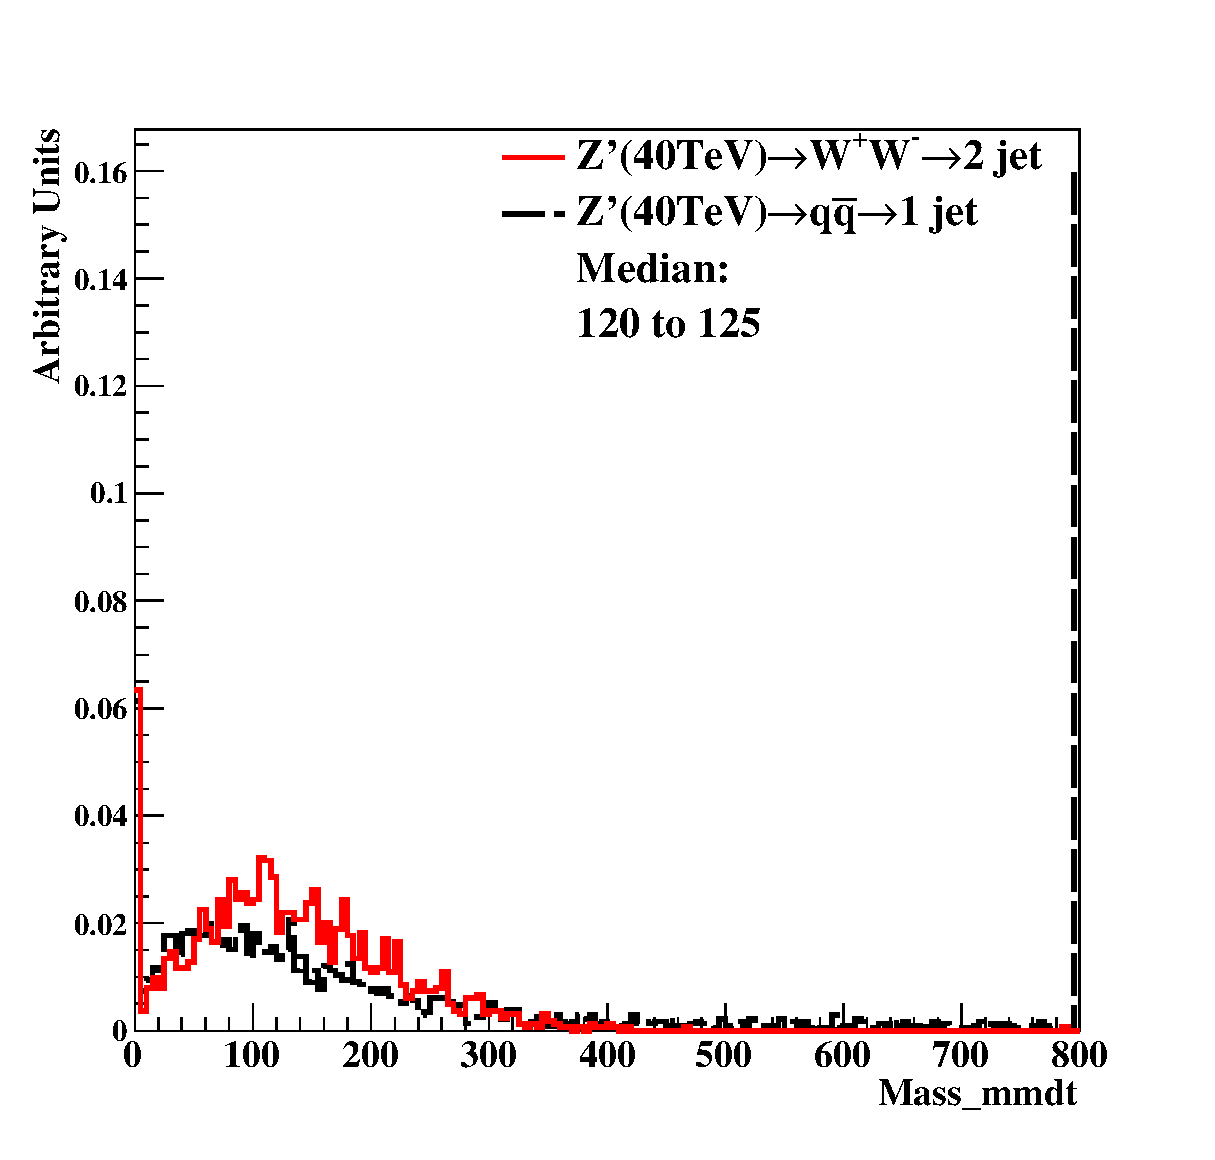
\includegraphics[width=0.22\textwidth]{figs/Dis_cluster_010_mass_mmdt_40tev_04_no_UOF.eps}
   }
   \subfigure[5TeV at 5$\times$5(cm$\times$cm) in cluster] {
   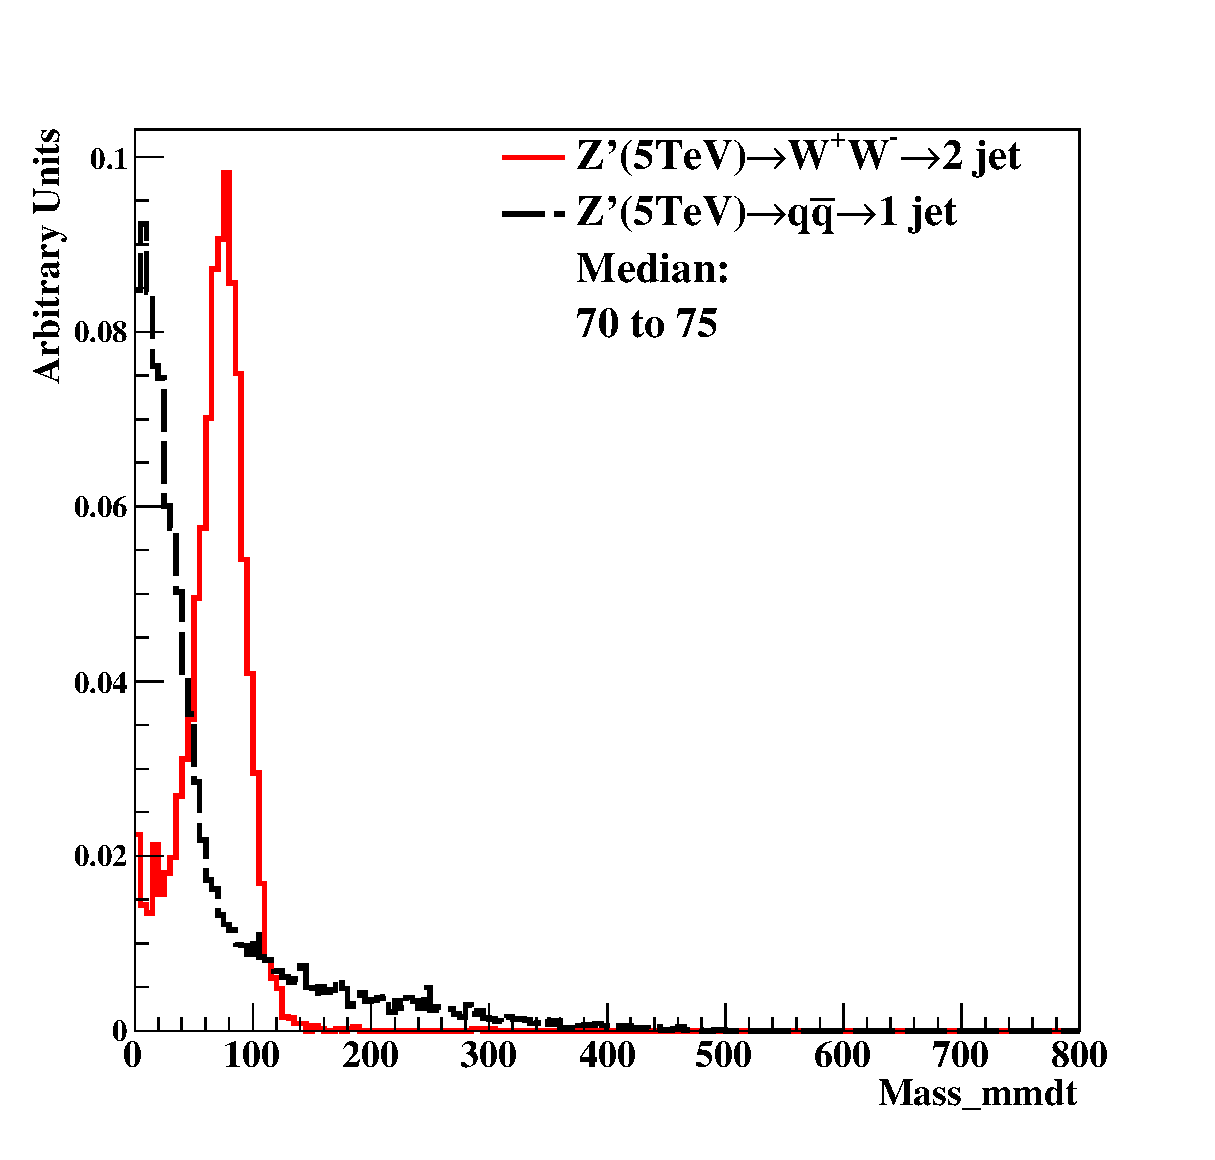
\includegraphics[width=0.22\textwidth]{figs/Dis_cluster_009_mass_mmdt_5tev_04_no_UOF.eps}
   }
   \subfigure[10TeV at 5$\times$5(cm$\times$cm) in cluster] {
   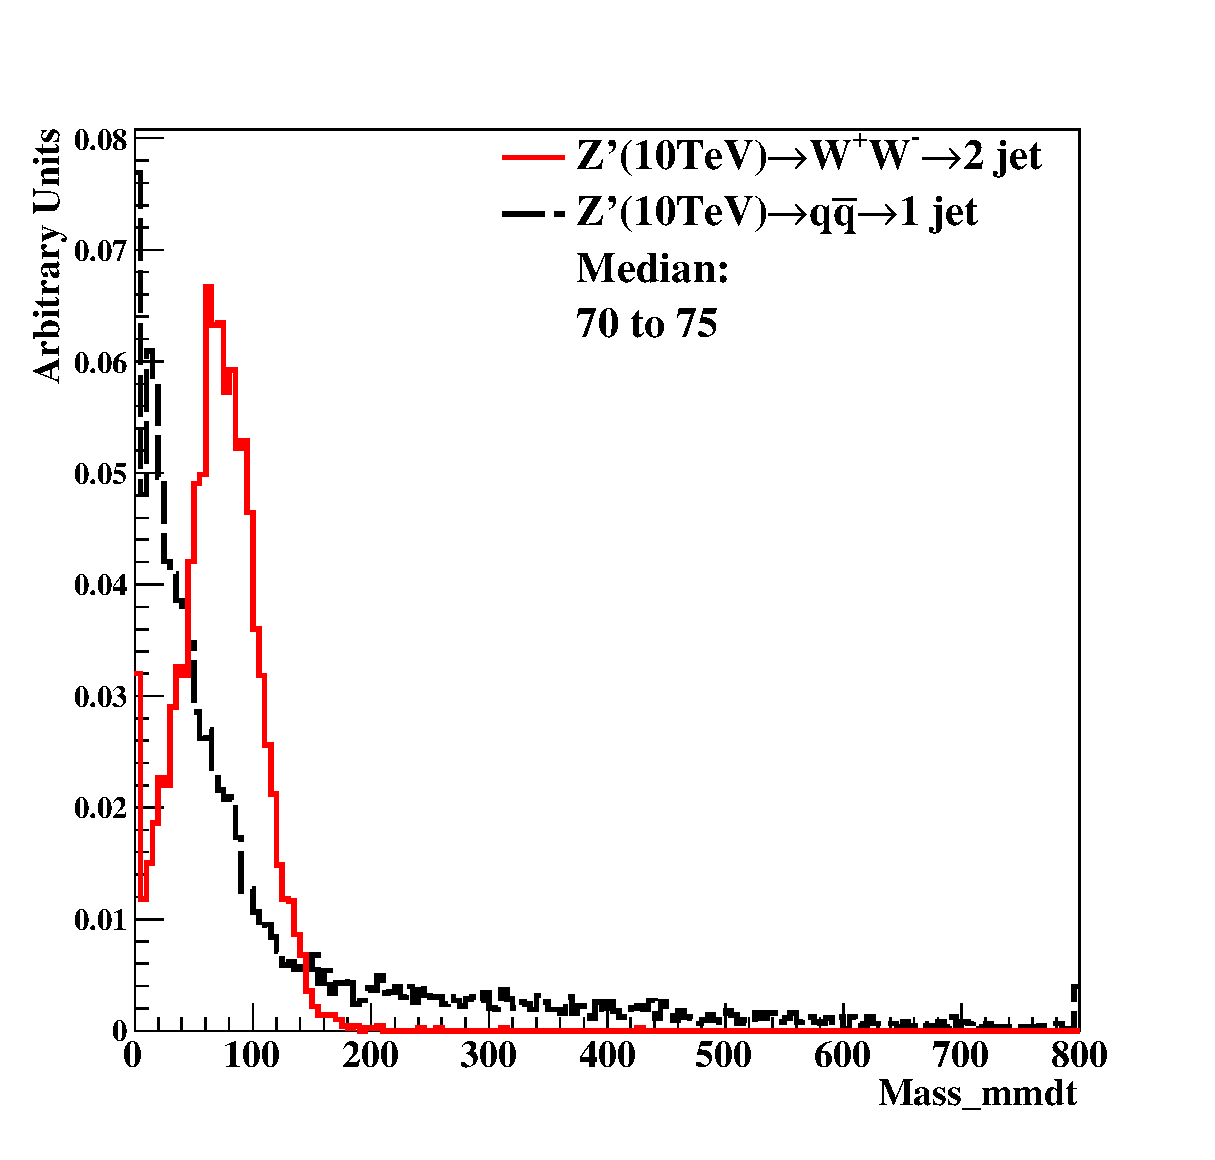
\includegraphics[width=0.22\textwidth]{figs/Dis_cluster_009_mass_mmdt_10tev_04_no_UOF.eps}
   }
      \subfigure[20TeV at 5$\times$5(cm$\times$cm) in cluster] {
   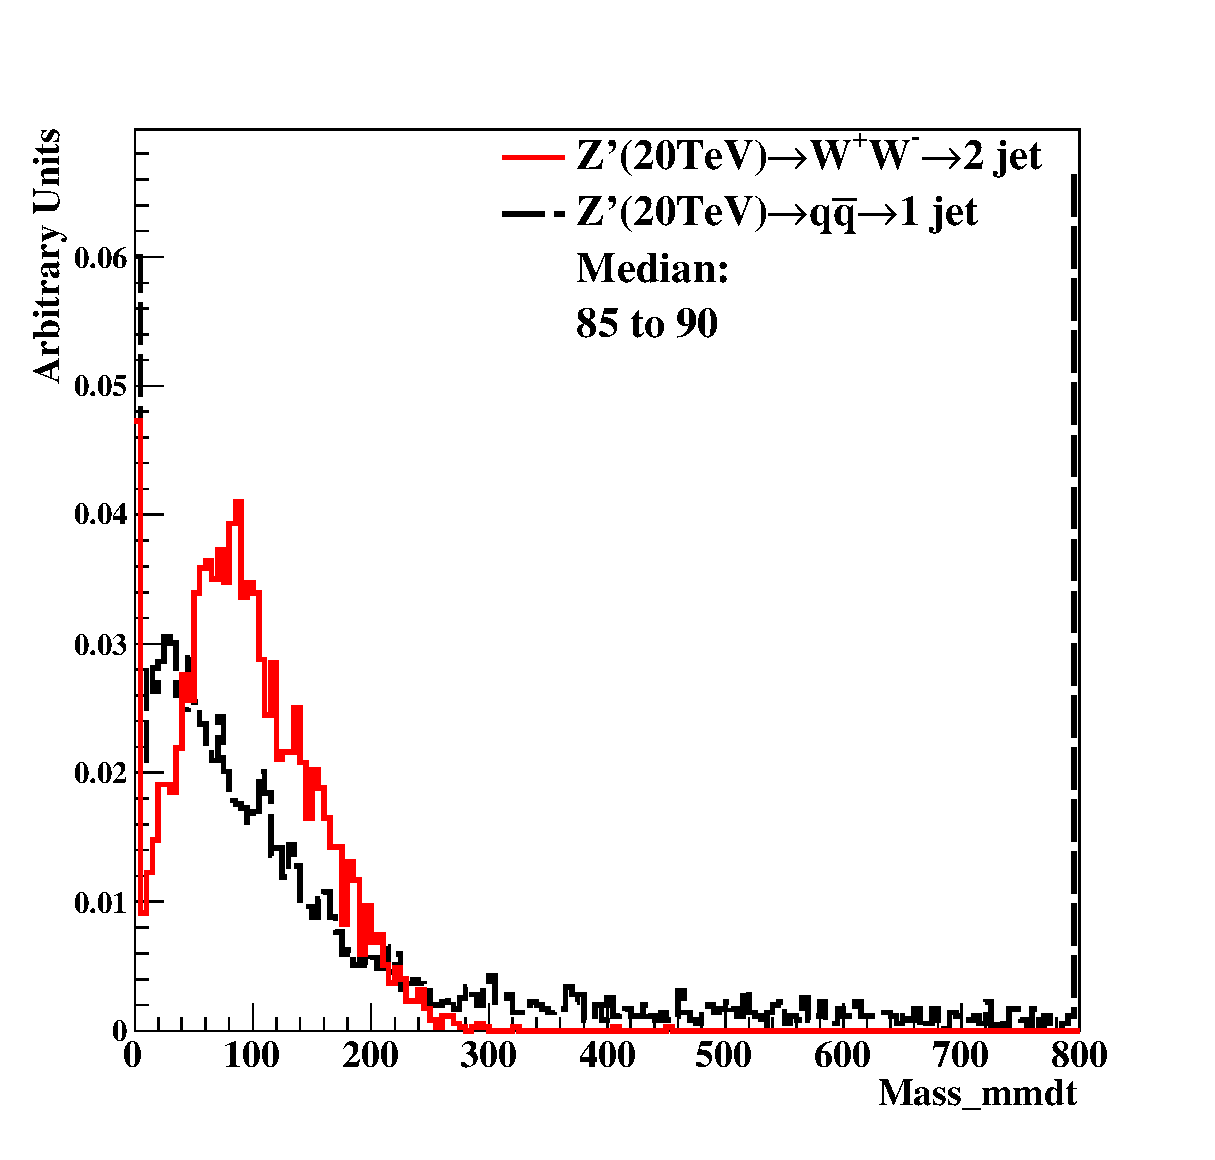
\includegraphics[width=0.22\textwidth]{figs/Dis_cluster_009_mass_mmdt_20tev_04_no_UOF.eps}\hfill
   }
      \subfigure[40TeV at 5$\times$5(cm$\times$cm) in cluster] {
   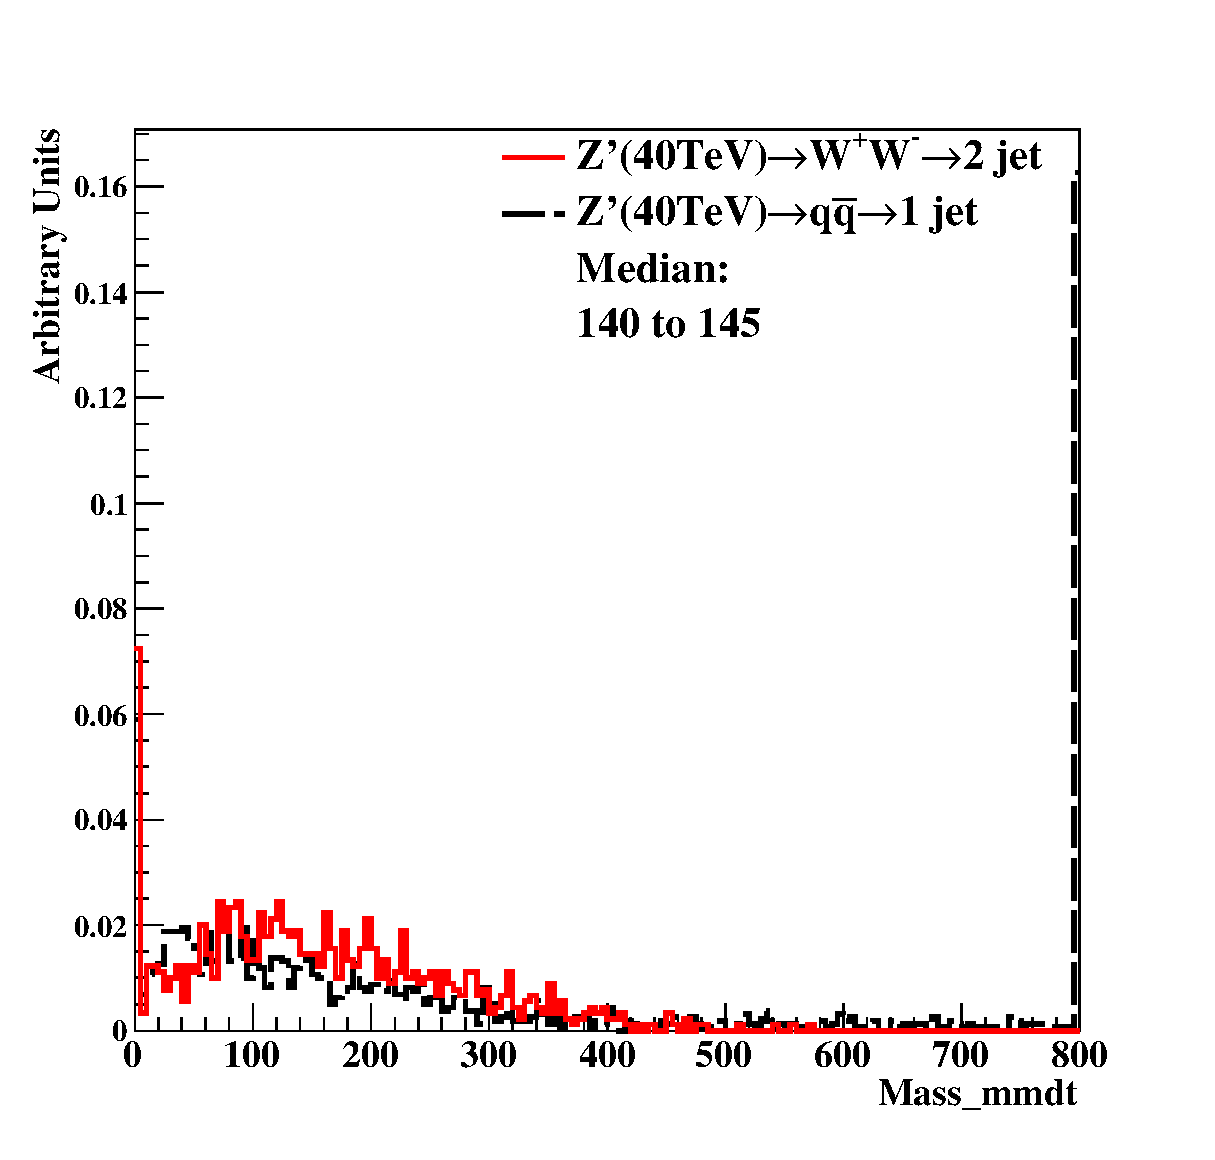
\includegraphics[width=0.22\textwidth]{figs/Dis_cluster_009_mass_mmdt_40tev_04_no_UOF.eps}\hfill
   }
   \subfigure[5TeV at 1$\times$1(cm$\times$cm) in cluster] {
   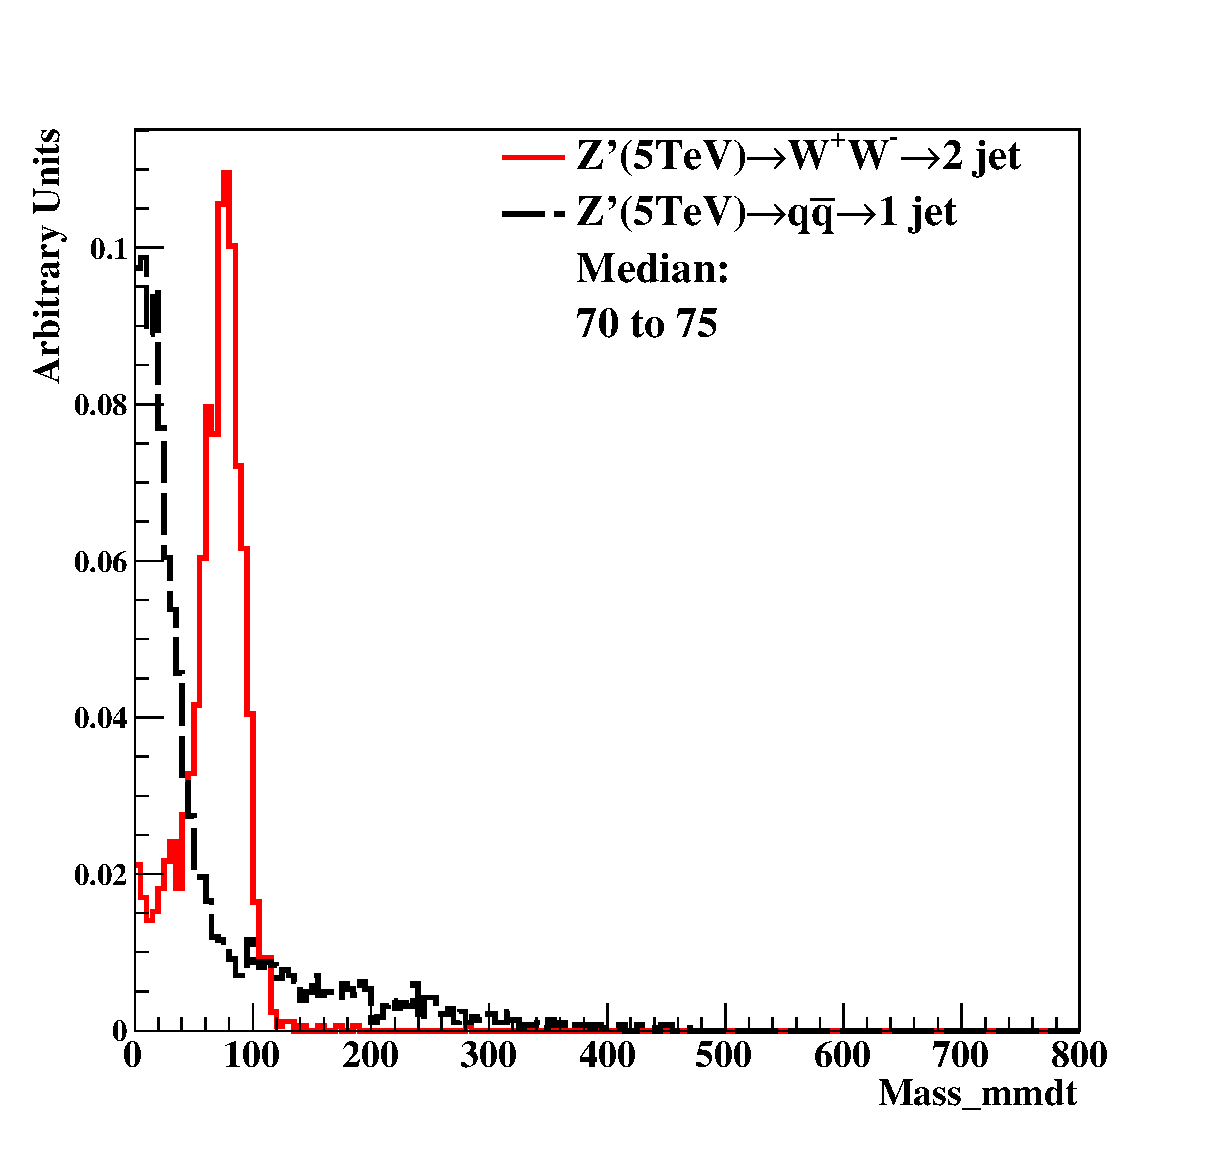
\includegraphics[width=0.22\textwidth]{figs/Dis_cluster_012_mass_mmdt_5tev_04_no_UOF.eps}\hfill
   }
    \subfigure[10TeV at 1$\times$1(cm$\times$cm) in cluster] {
   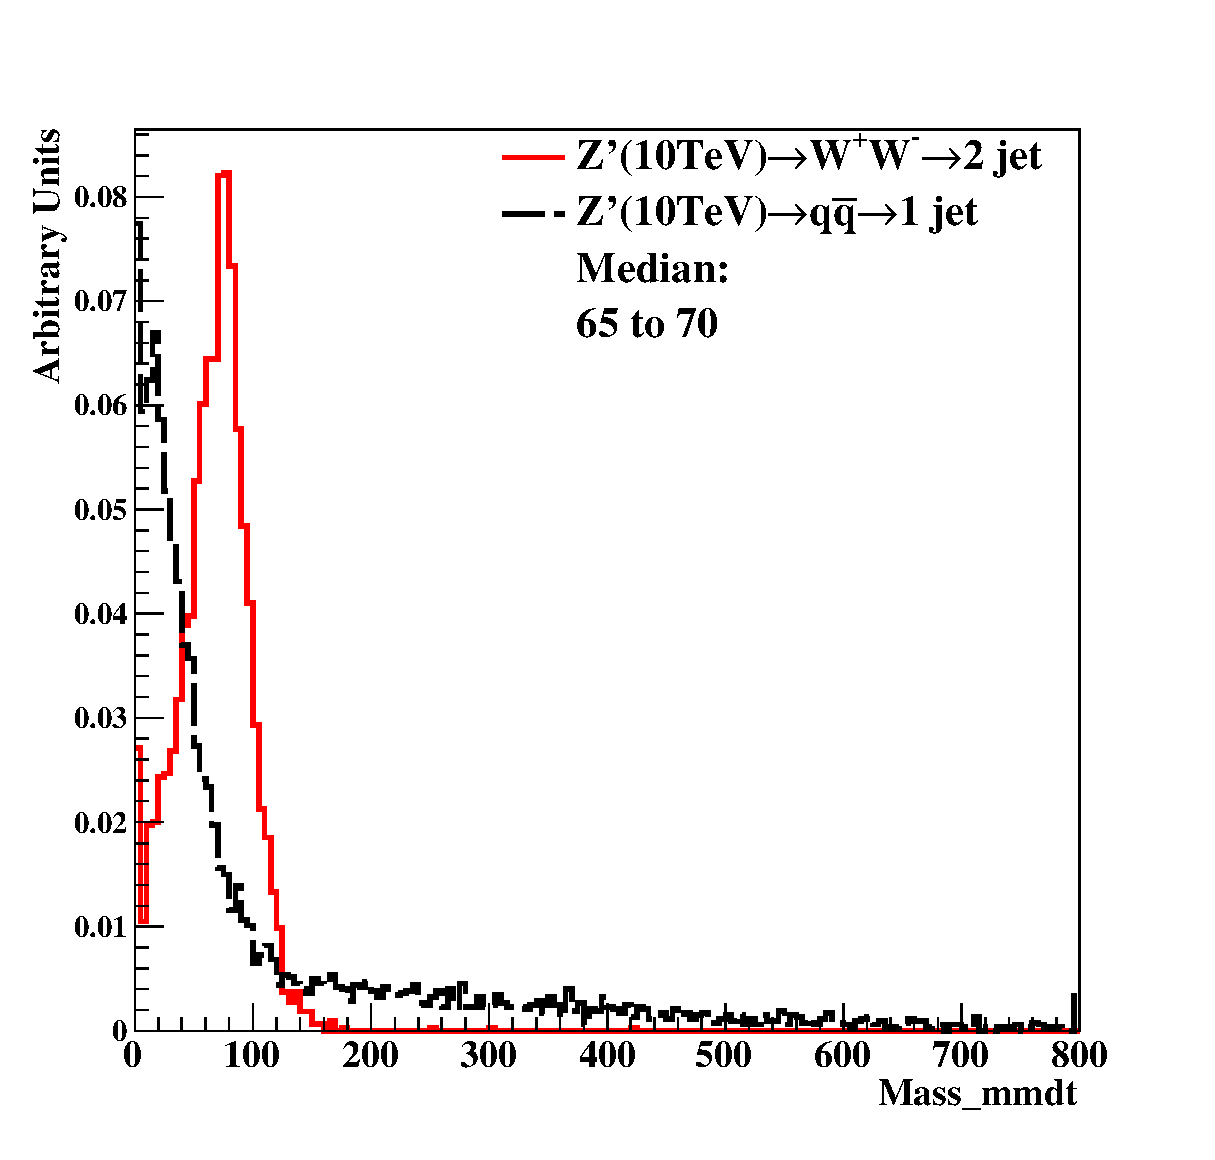
\includegraphics[width=0.22\textwidth]{figs/Dis_cluster_012_mass_mmdt_10tev_04_no_UOF.eps}
   }
   \subfigure[20TeV at 1$\times$1(cm$\times$cm) in cluster] {
   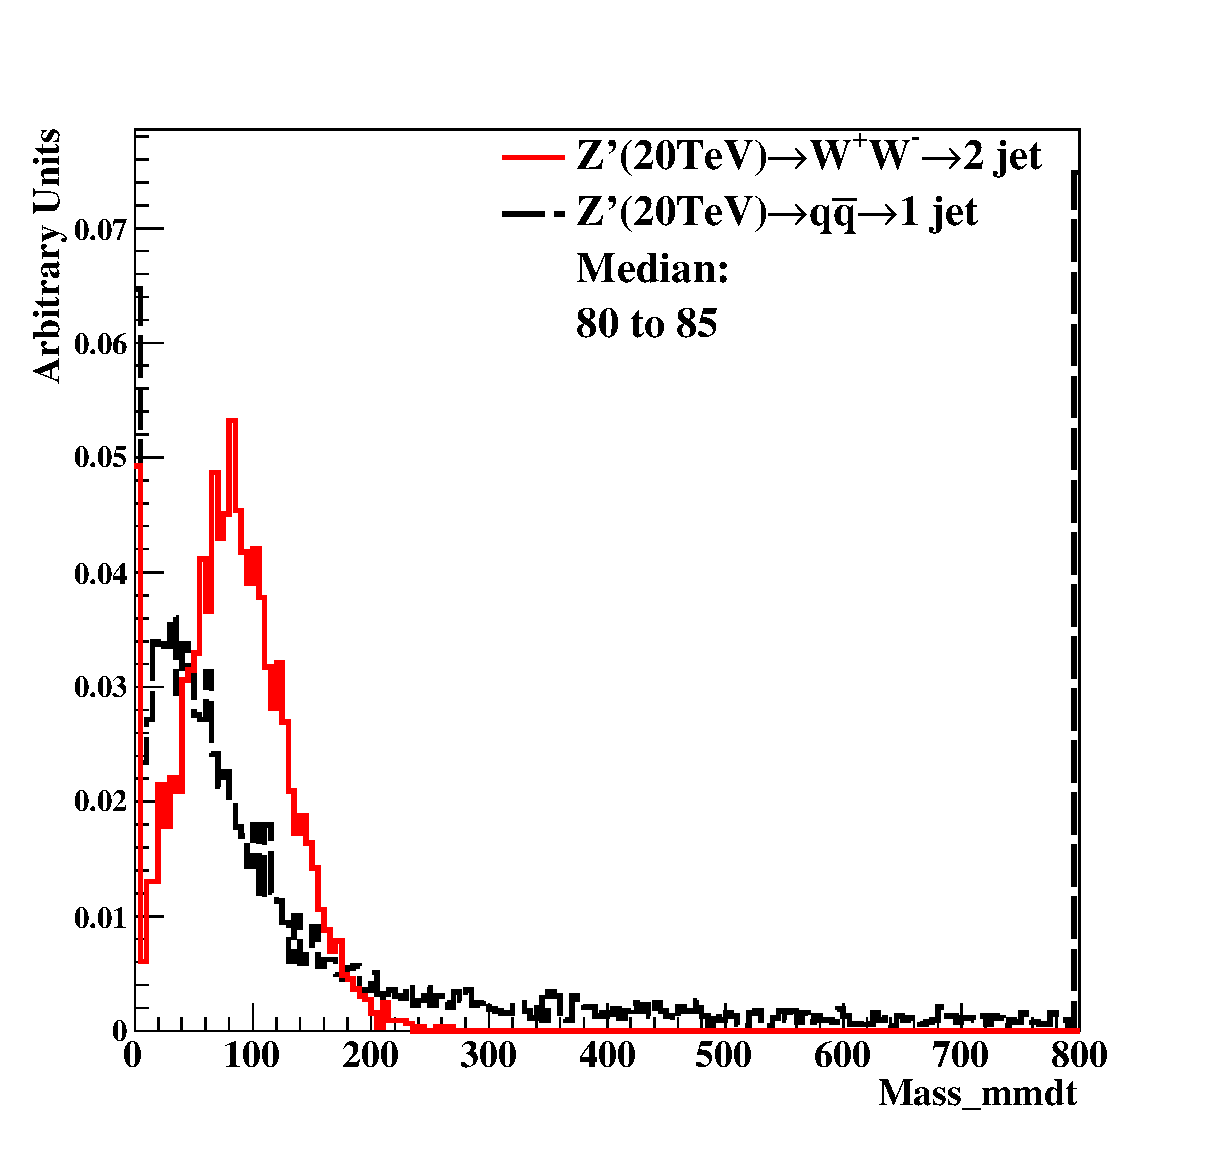
\includegraphics[width=0.22\textwidth]{figs/Dis_cluster_012_mass_mmdt_20tev_04_no_UOF.eps}\hfill
   }
      \subfigure[40TeV at 1$\times$1(cm$\times$cm) in cluster] {
   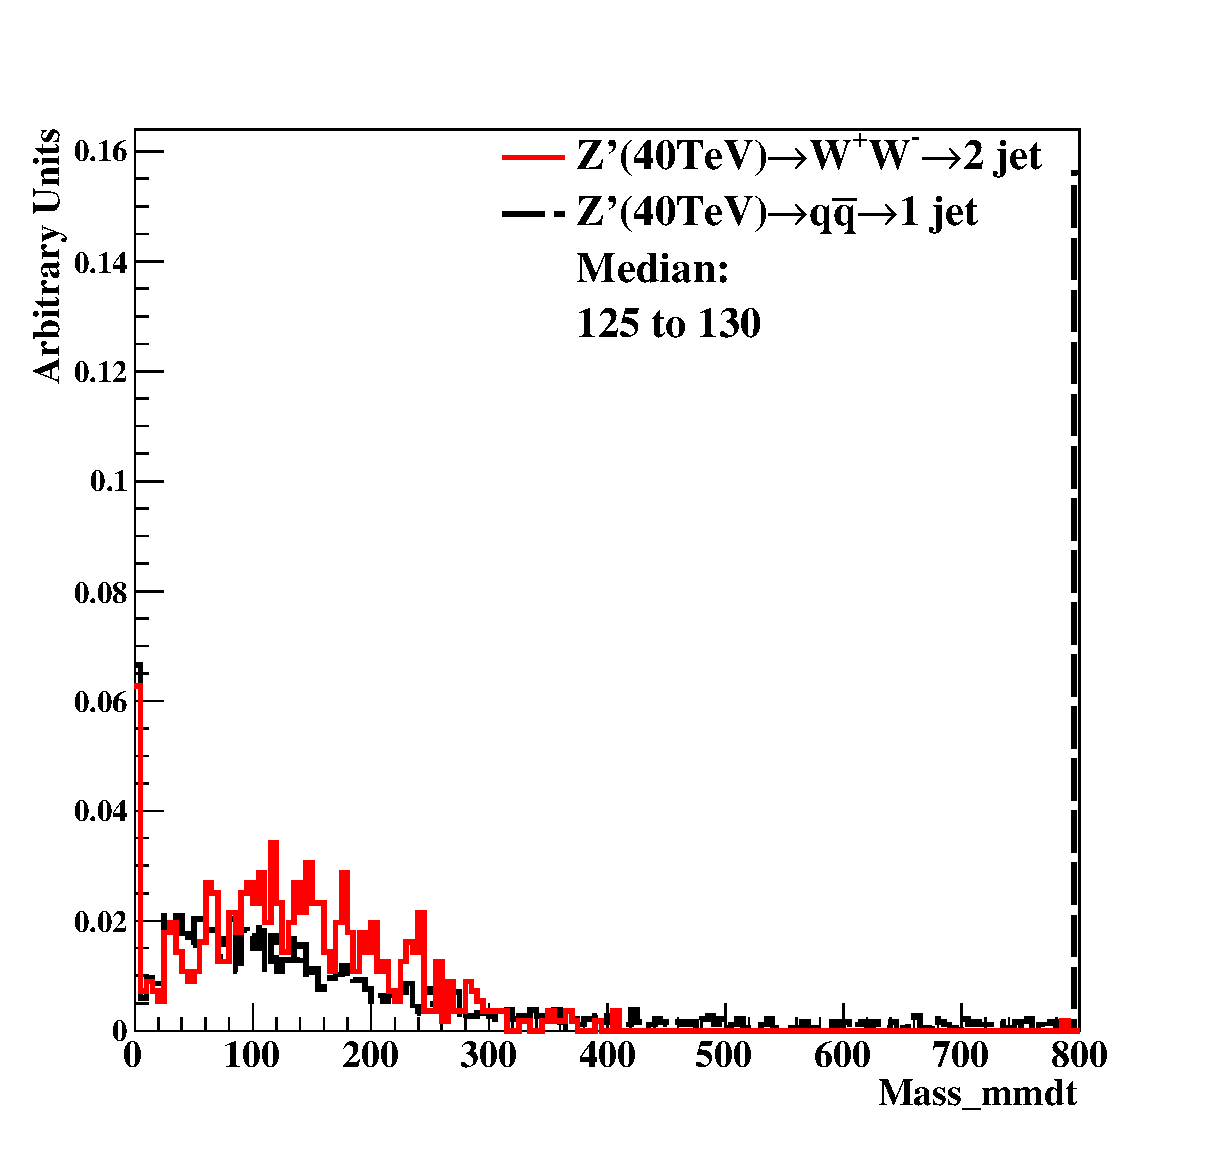
\includegraphics[width=0.22\textwidth]{figs/Dis_cluster_012_mass_mmdt_40tev_04_no_UOF.eps}
   }

\end{center}
\caption{Distributions of mass soft drop at $\beta$=0, signal=ww, in 5,10TeV energy of collision  in different detector sizes. Cell Size in 20$\times$20, 5$\times$5, and 1$\times$1(cm$\times$cm) are shown here.}
\label{fig:cluster_tau21_tau32}
\end{figure}


\begin{figure}
\begin{center}
  \subfigure[Central at Median($20\times20$=,$5\times5$=,$1\times1$=) change width in cluster at 5TeV] {
  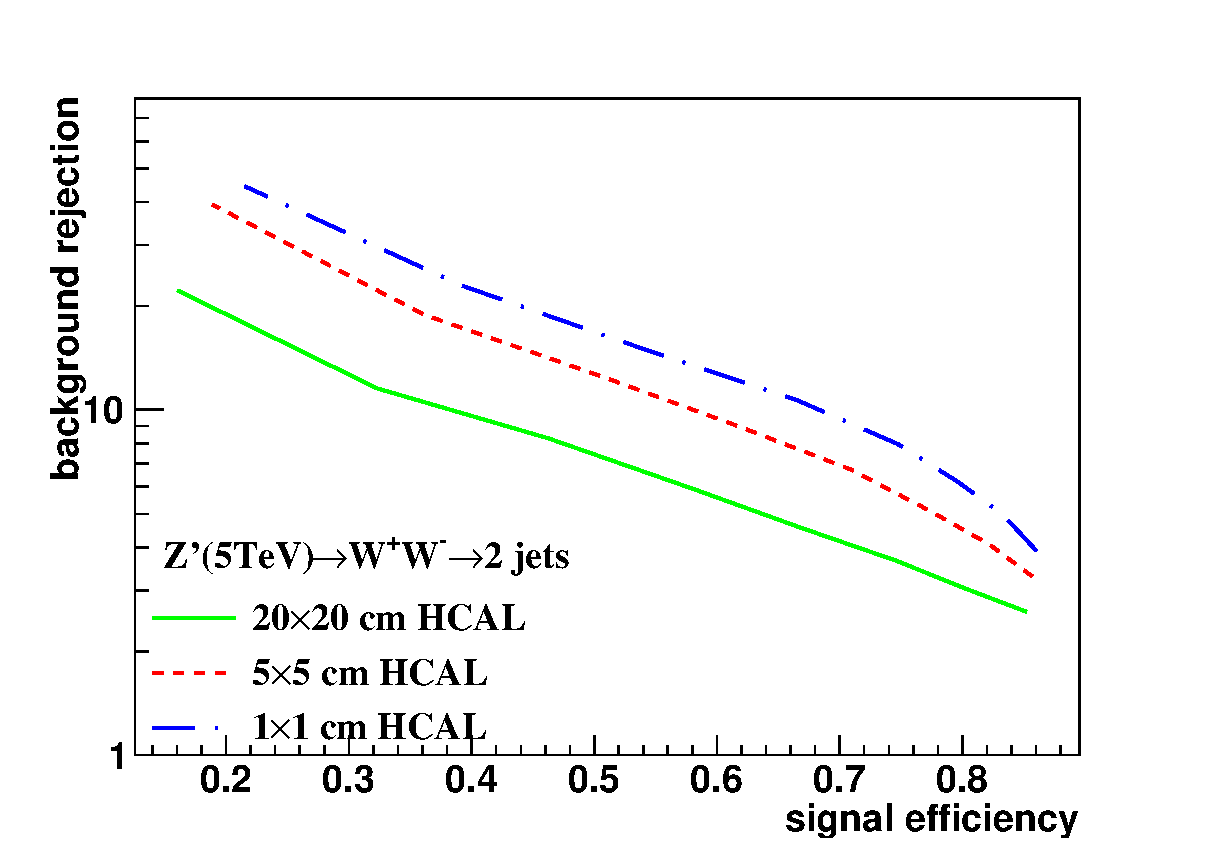
\includegraphics[width=0.43\textwidth]{figs/A_Cluster_mass_mmdt_5tev_eff_1_central_fix_ww_qq_log_no_UOF.eps}
  }
  \subfigure[Central at Median($20\times20$=,$5\times5$=,$1\times1$=) change width in cluster at 10TeV] {
  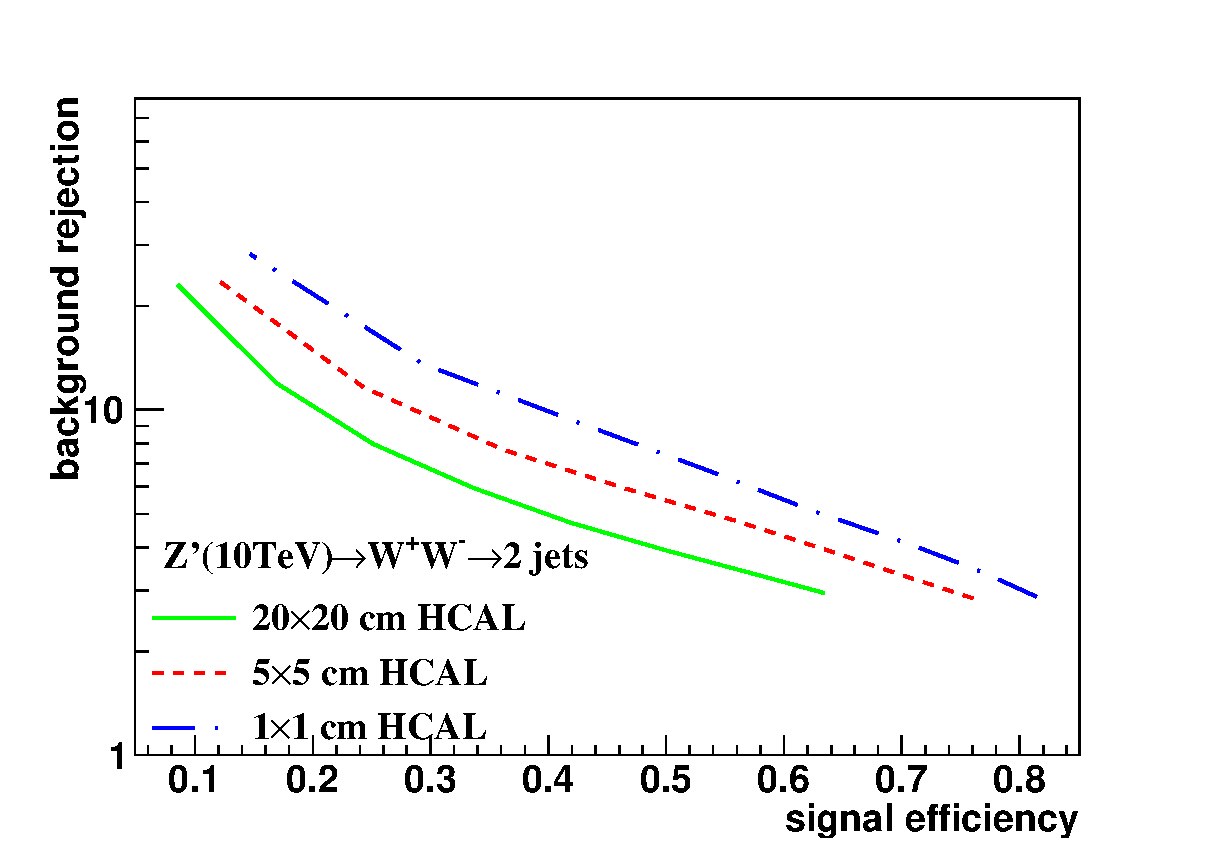
\includegraphics[width=0.43\textwidth]{figs/A_Cluster_mass_mmdt_10tev_eff_1_central_fix_ww_qq_log_no_UOF.eps}
  }
 \subfigure[Central at Median($20\times20$=,$5\times5$=,$1\times1$=) change width in cluster at 20TeV] {
 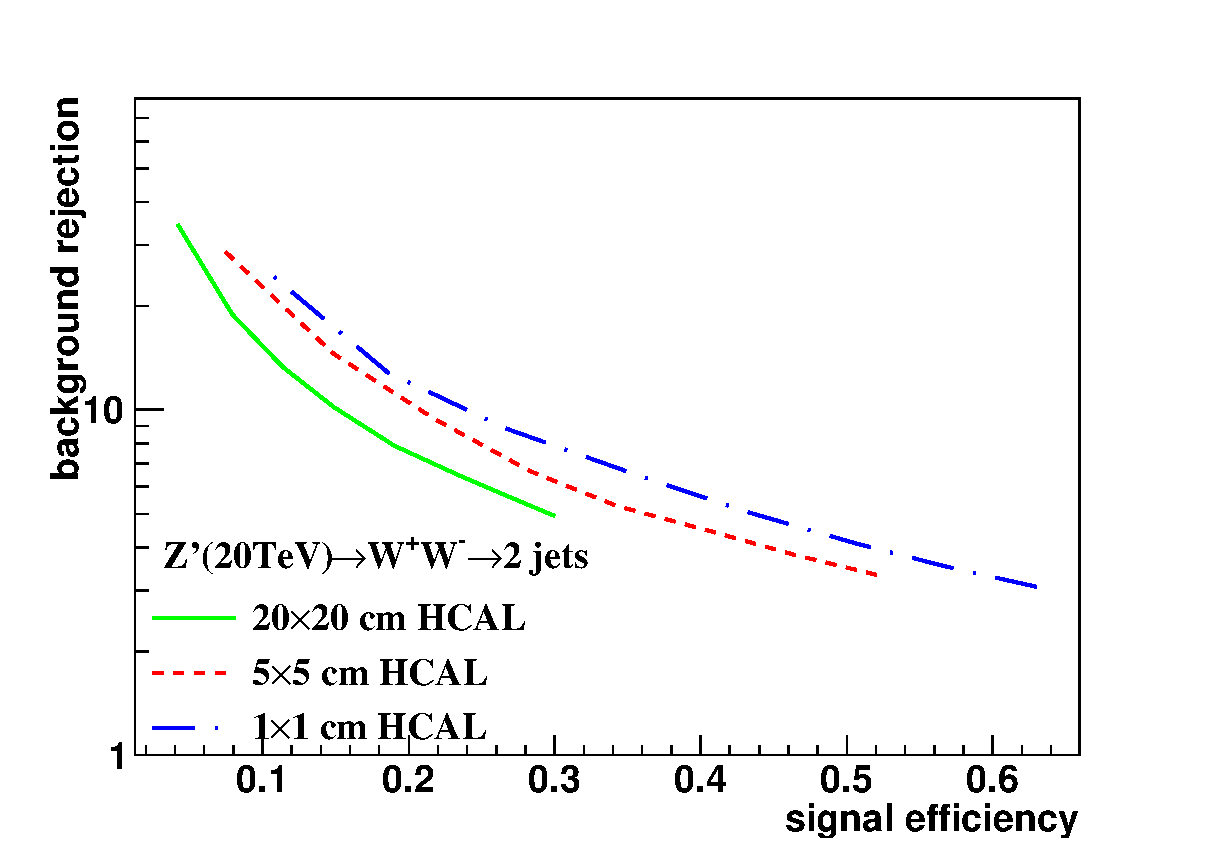
\includegraphics[width=0.43\textwidth]{figs/A_Cluster_mass_mmdt_20tev_eff_1_central_fix_ww_qq_log_no_UOF.eps}
 }
 \subfigure[Central at Median($20\times20$=,$5\times5$=,$1\times1$=) change width in cluster at 40TeV] {
 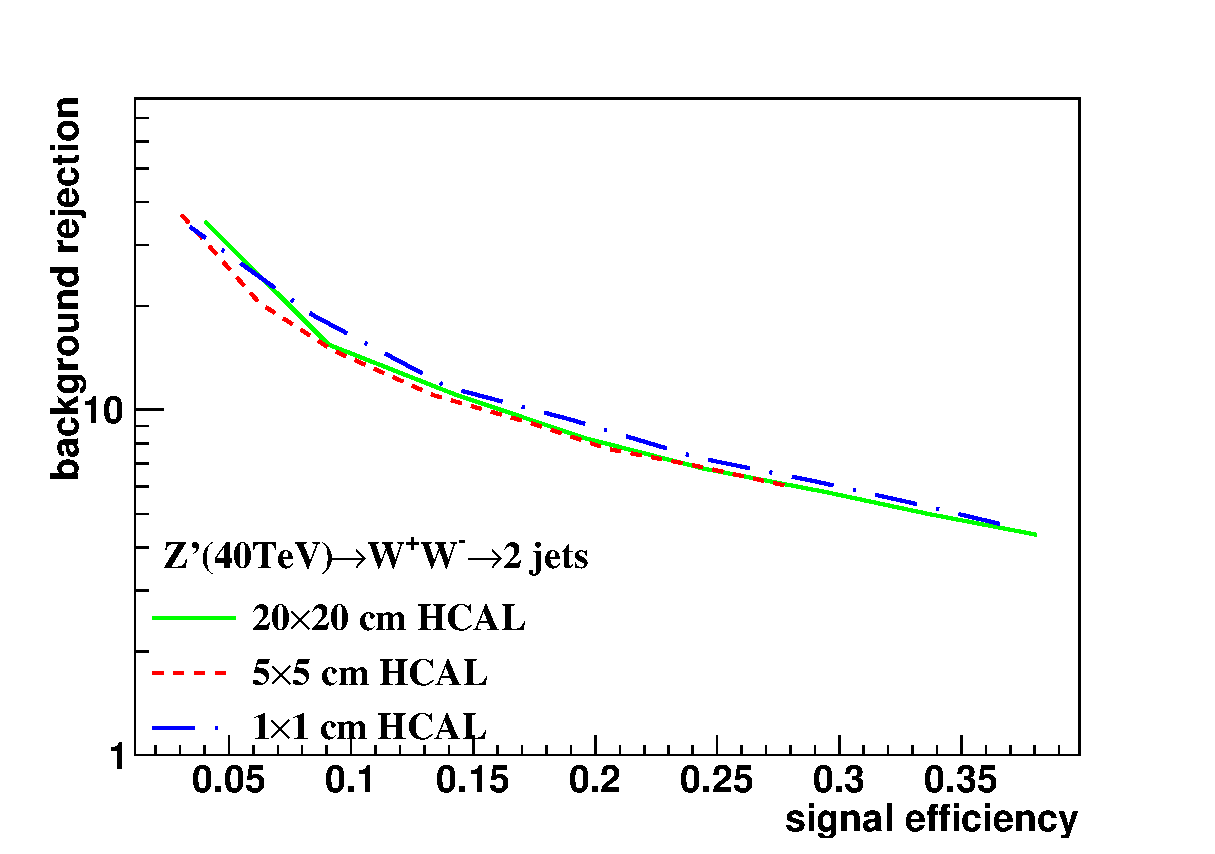
\includegraphics[width=0.43\textwidth]{figs/A_Cluster_mass_mmdt_40tev_eff_1_central_fix_ww_qq_log_no_UOF.eps}
 }
\end{center}
\caption{study of "fix central and change width" in mass soft drop at $\beta$=0, signal=ww, in 5, 10, 20, 40TeV energy of collision  in different detector sizes. Cell Size in 20$\times$20, 5$\times$5, and 1$\times$1(cm$\times$cm) are shown in each picture.}
\label{fig:cluster_tau21_tau32}
\end{figure}


\begin{figure}
\begin{center}
   \subfigure[5TeV at 20$\times$20(cm$\times$cm) in cluster] {
   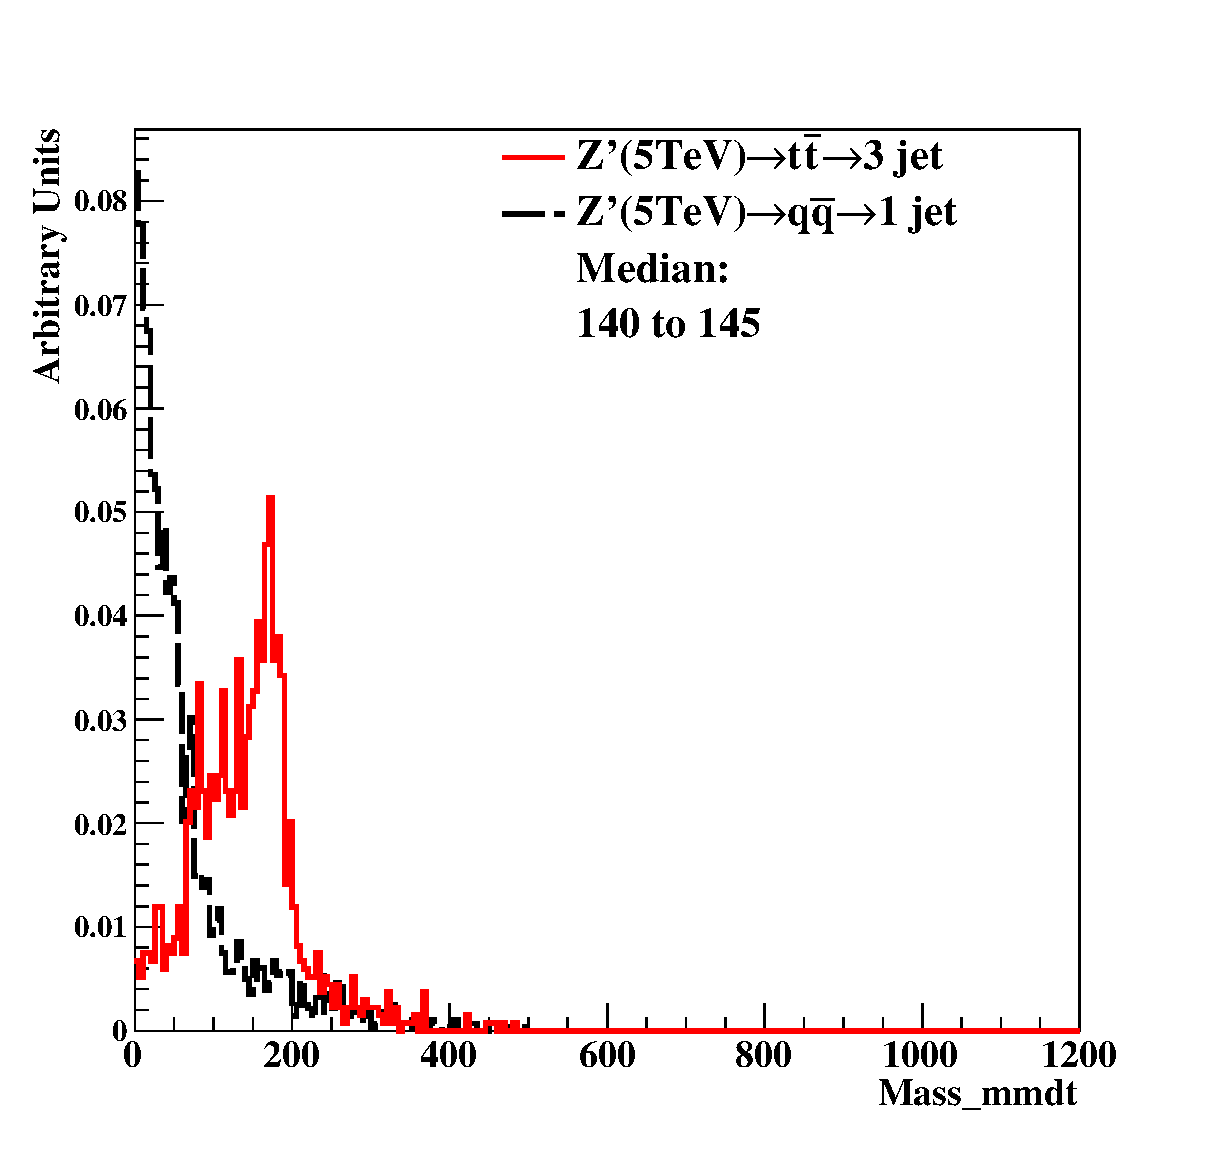
\includegraphics[width=0.22\textwidth]{figs/Dis_cluster_010_mass_mmdt_tt_5tev_04_tt_no_UOF.eps}
   }
      \subfigure[10TeV at 20$\times$20(cm$\times$cm) in cluster] {
   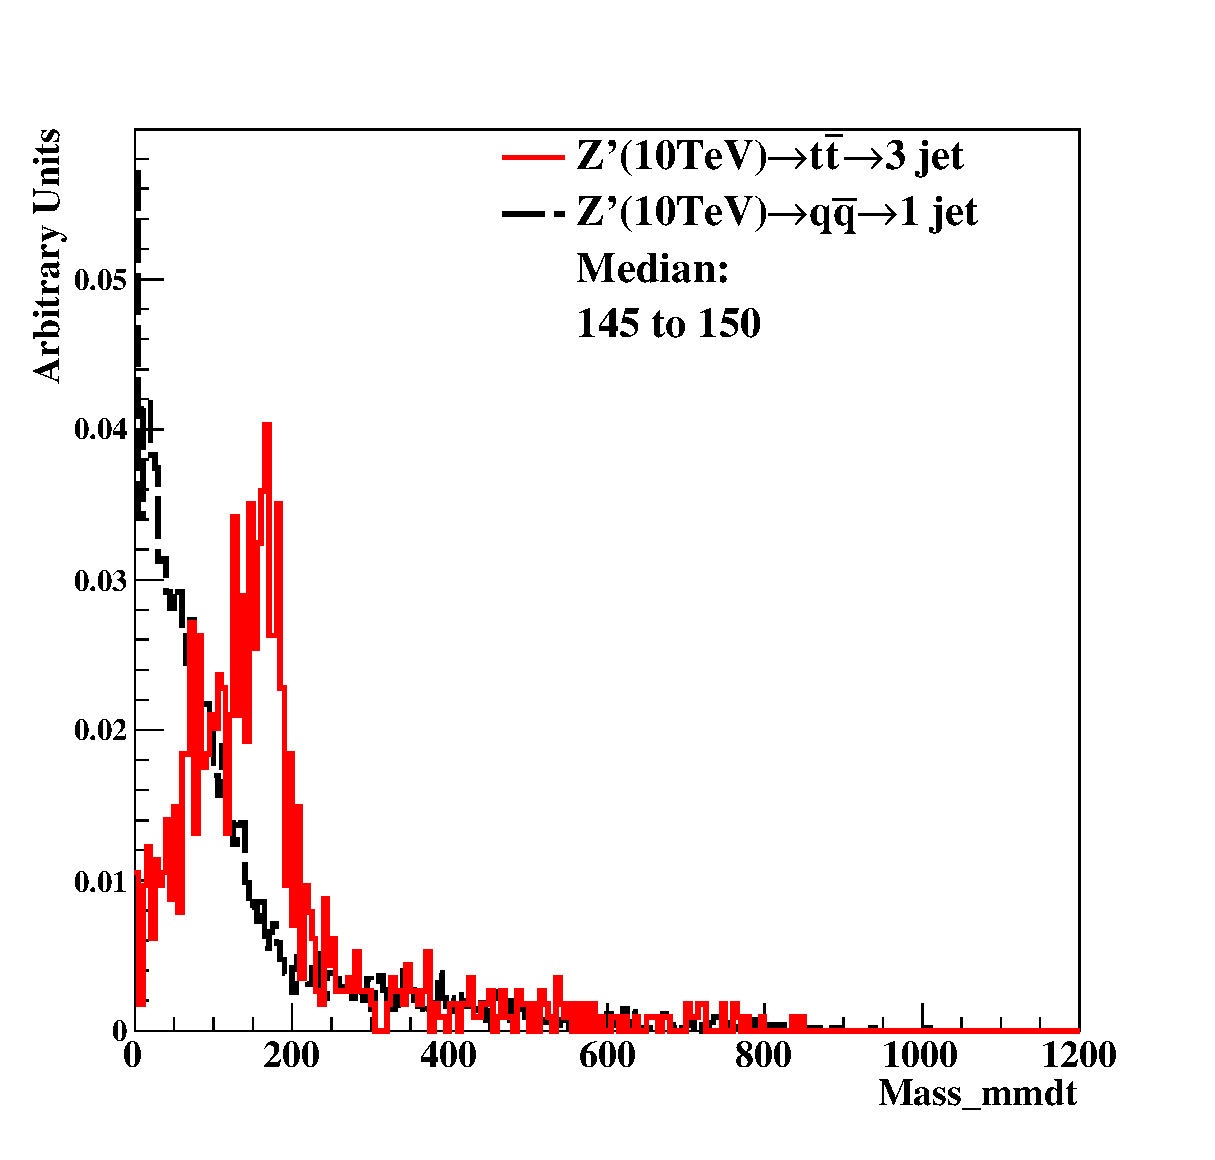
\includegraphics[width=0.22\textwidth]{figs/Dis_cluster_010_mass_mmdt_tt_10tev_04_tt_no_UOF.eps}
   }
   \subfigure[20TeV at 5$\times$5(cm$\times$cm) in cluster] {
   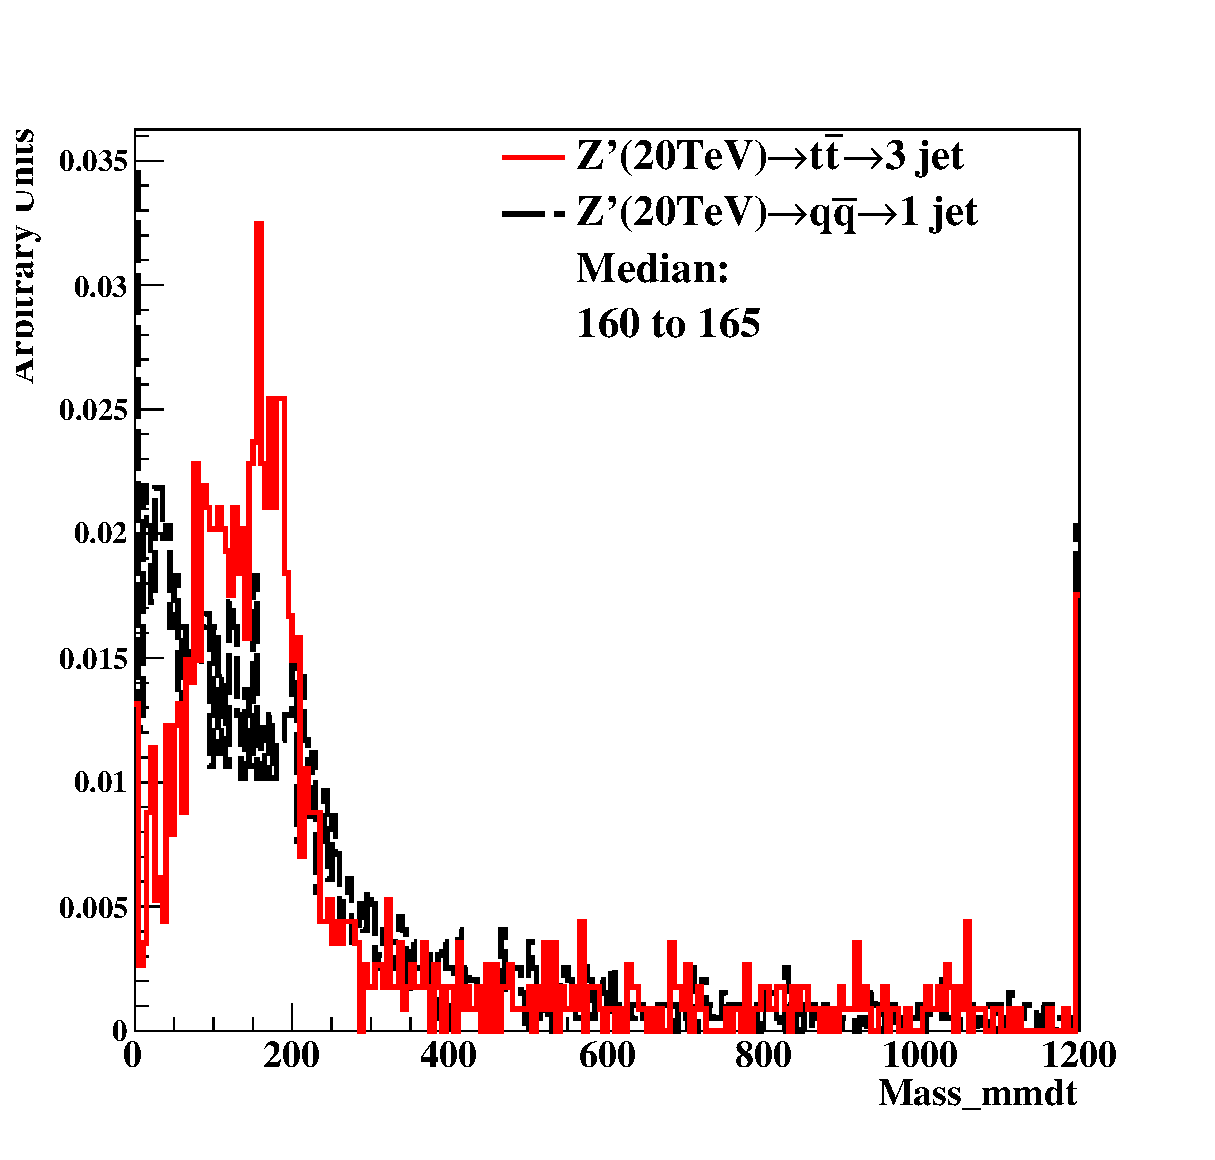
\includegraphics[width=0.22\textwidth]{figs/Dis_cluster_010_mass_mmdt_tt_20tev_04_tt_no_UOF.eps}
   }
    \subfigure[40TeV at 5$\times$5(cm$\times$cm) in cluster] {
   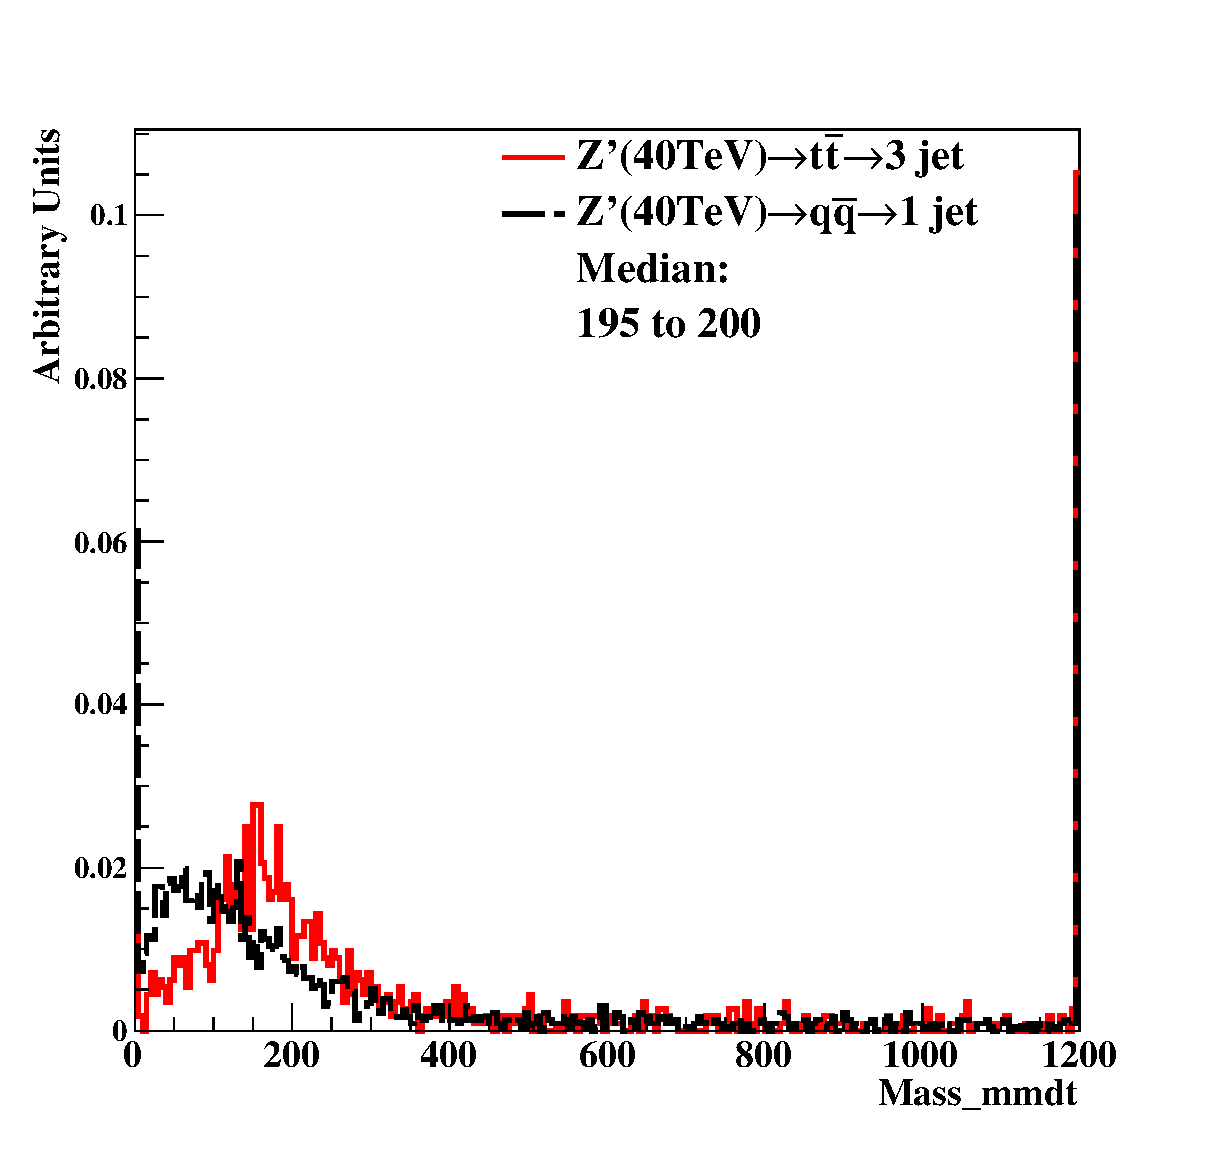
\includegraphics[width=0.22\textwidth]{figs/Dis_cluster_010_mass_mmdt_tt_40tev_04_tt_no_UOF.eps}
   }
   \subfigure[5TeV at 1$\times$1(cm$\times$cm) in cluster] {
   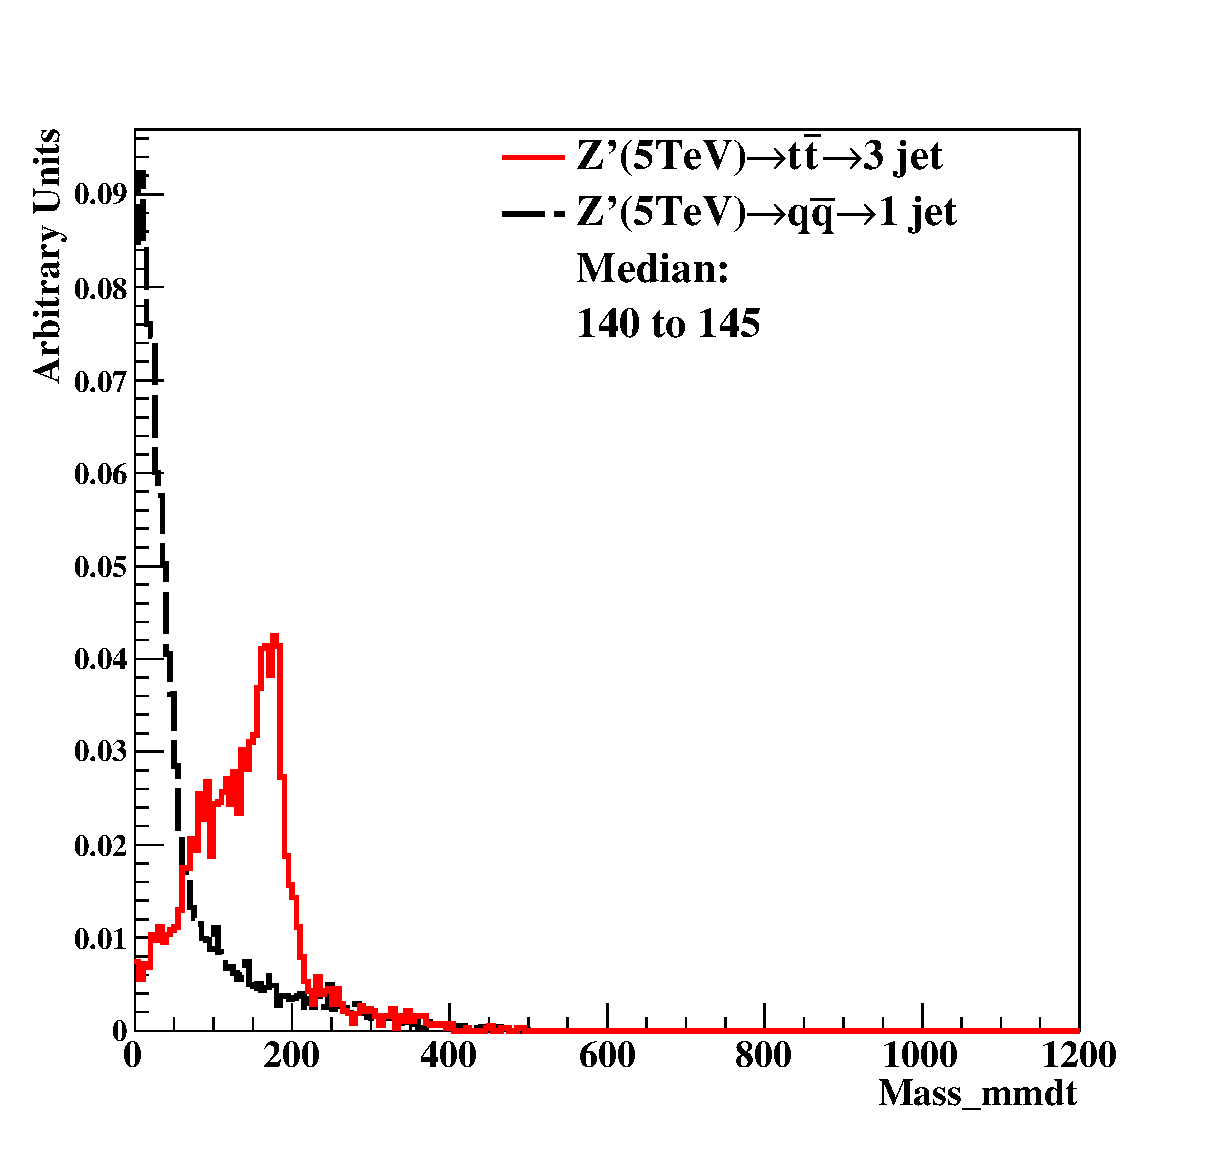
\includegraphics[width=0.22\textwidth]{figs/Dis_cluster_009_mass_mmdt_tt_5tev_04_tt_no_UOF.eps}
   }
   \subfigure[10TeV at 1$\times$1(cm$\times$cm) in cluster] {
   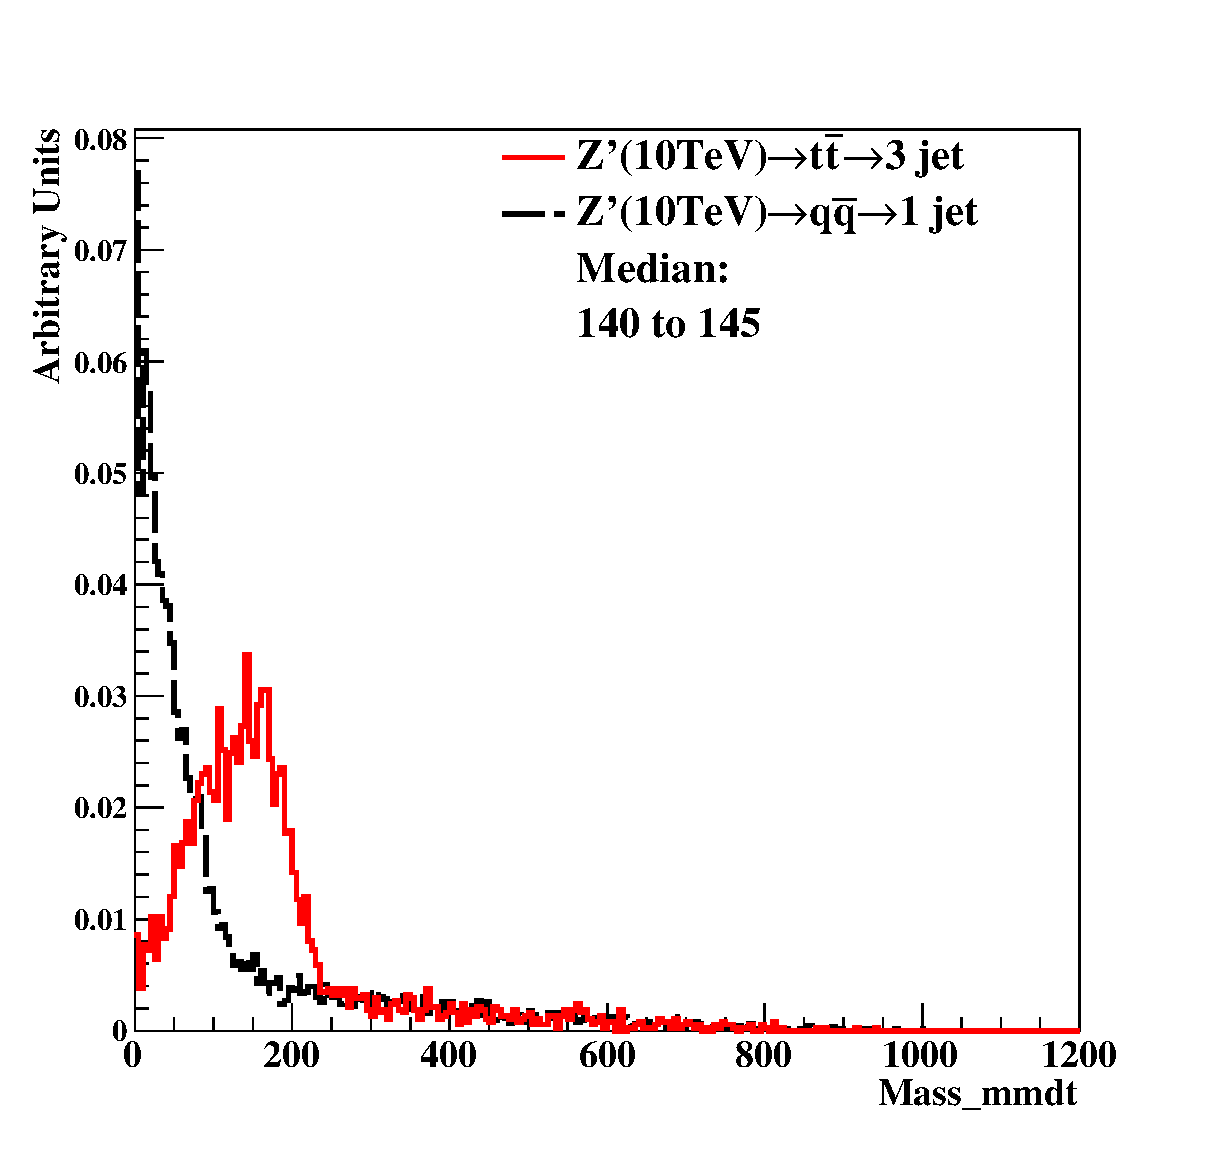
\includegraphics[width=0.22\textwidth]{figs/Dis_cluster_009_mass_mmdt_tt_10tev_04_tt_no_UOF.eps}
   }
   \subfigure[20TeV at 20$\times$20(cm$\times$cm) in cluster] {
   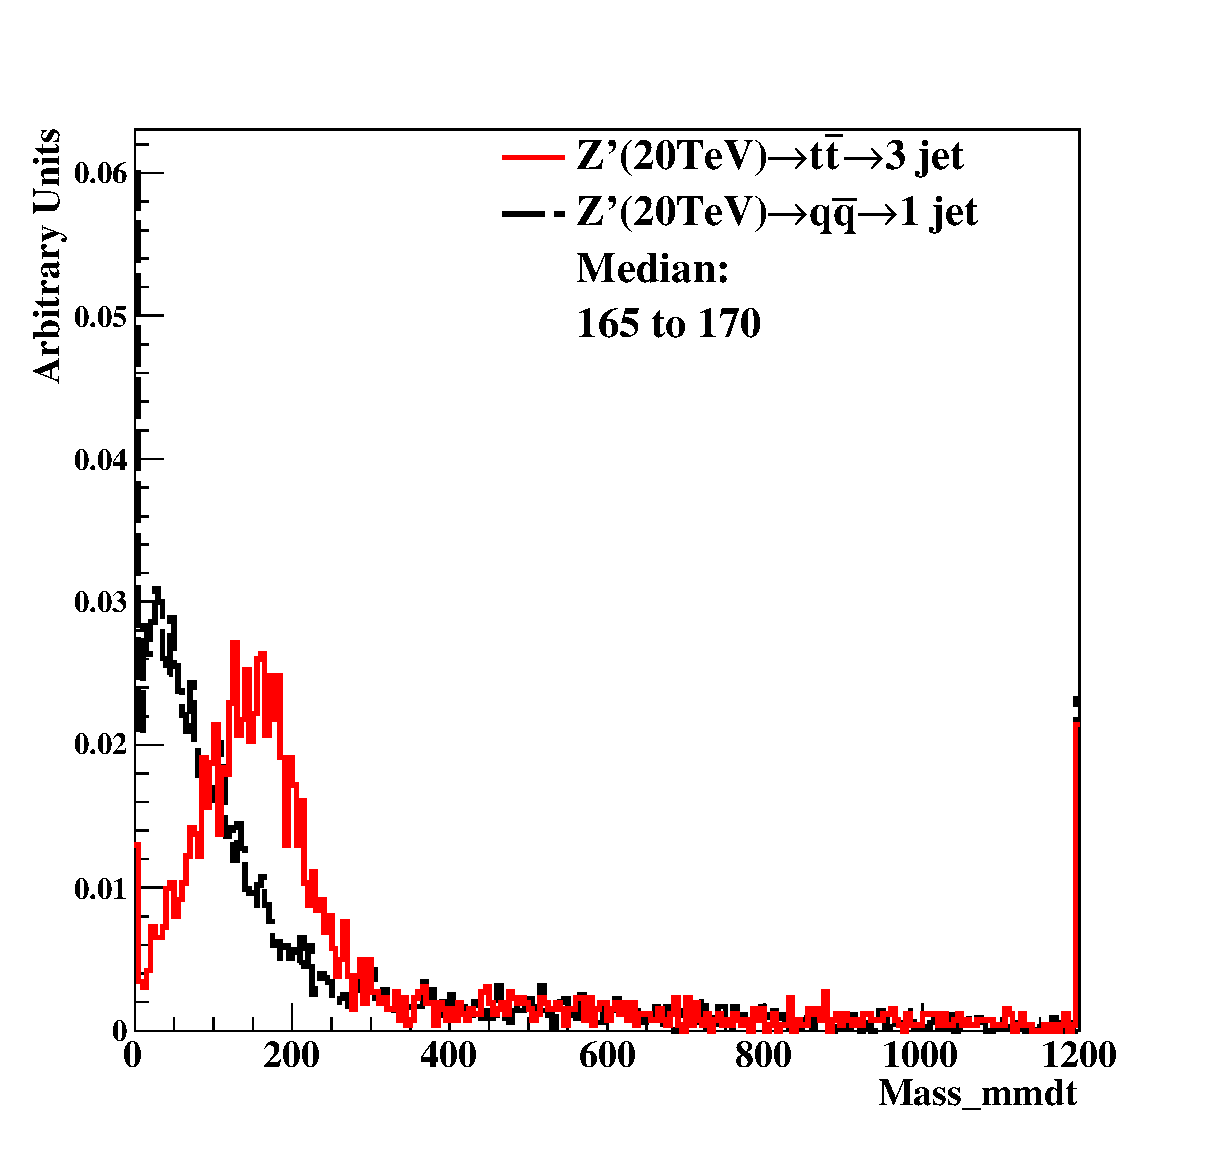
\includegraphics[width=0.22\textwidth]{figs/Dis_cluster_009_mass_mmdt_tt_20tev_04_tt_no_UOF.eps}\hfill
   }
      \subfigure[40TeV at 20$\times$20(cm$\times$cm) in cluster] {
   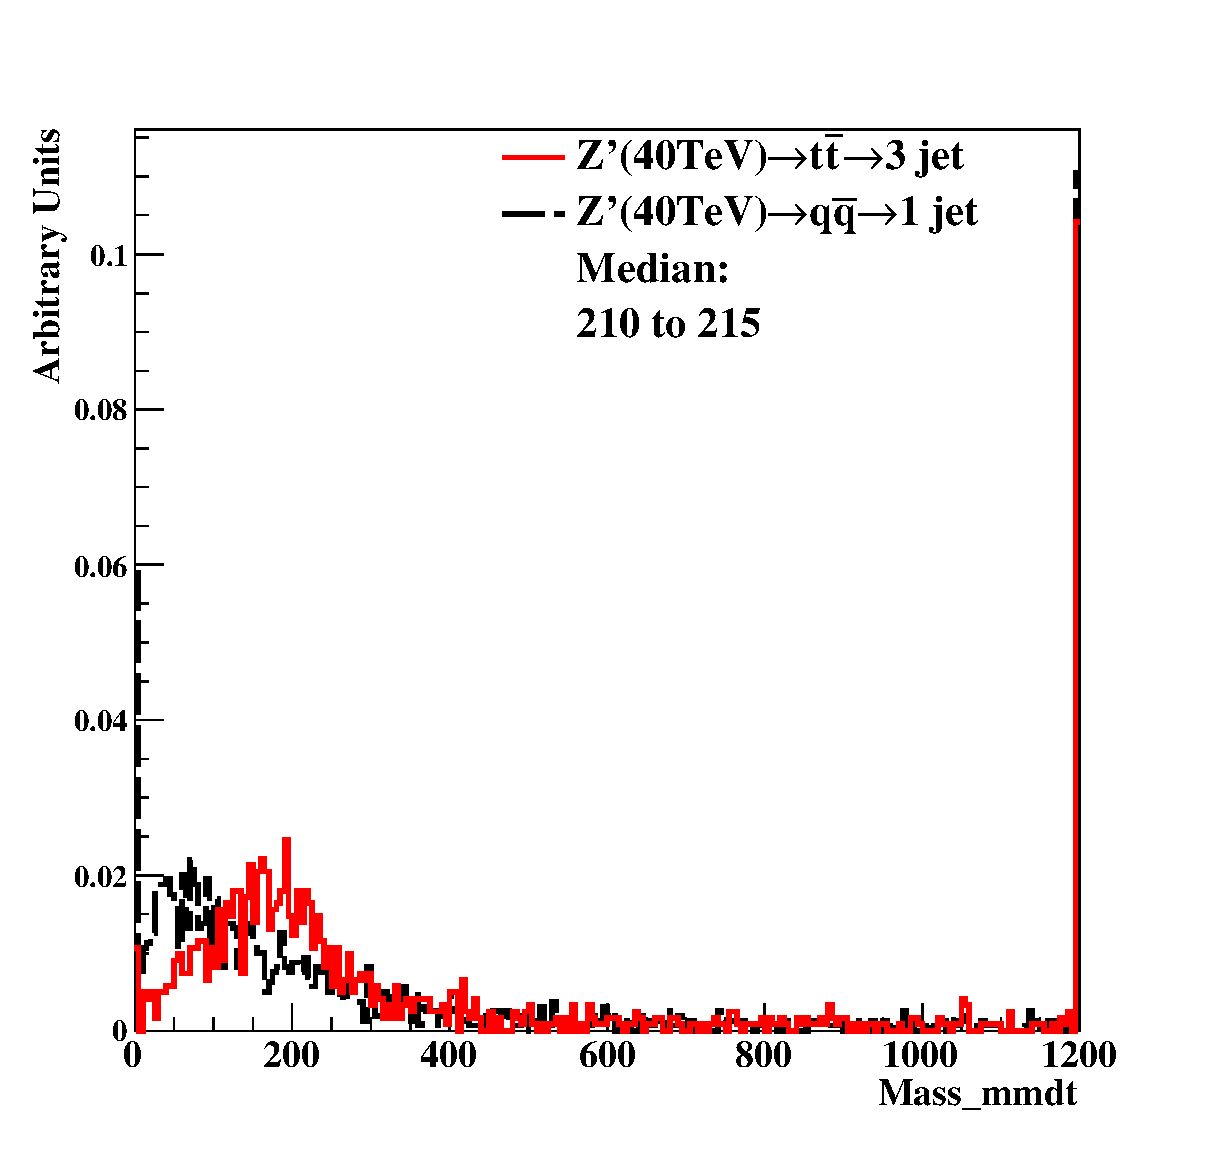
\includegraphics[width=0.22\textwidth]{figs/Dis_cluster_009_mass_mmdt_tt_40tev_04_tt_no_UOF.eps}\hfill
   }
   \subfigure[5TeV at 5$\times$5(cm$\times$cm) in cluster] {
   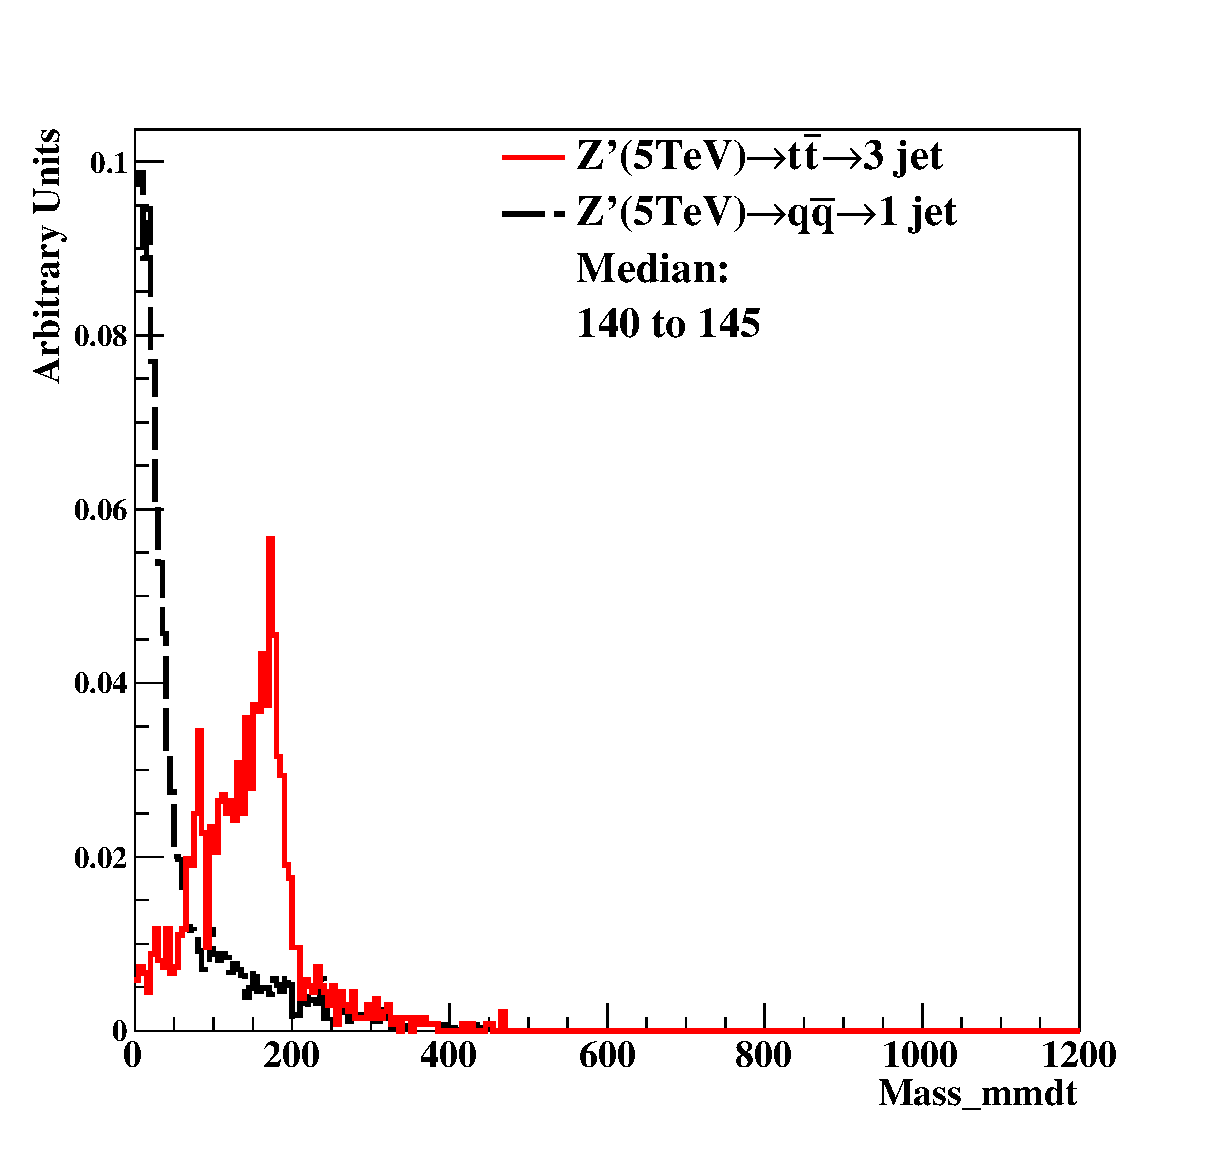
\includegraphics[width=0.22\textwidth]{figs/Dis_cluster_012_mass_mmdt_tt_5tev_04_tt_no_UOF.eps}\hfill
   }
    \subfigure[10TeV at 5$\times$5(cm$\times$cm) in cluster] {
   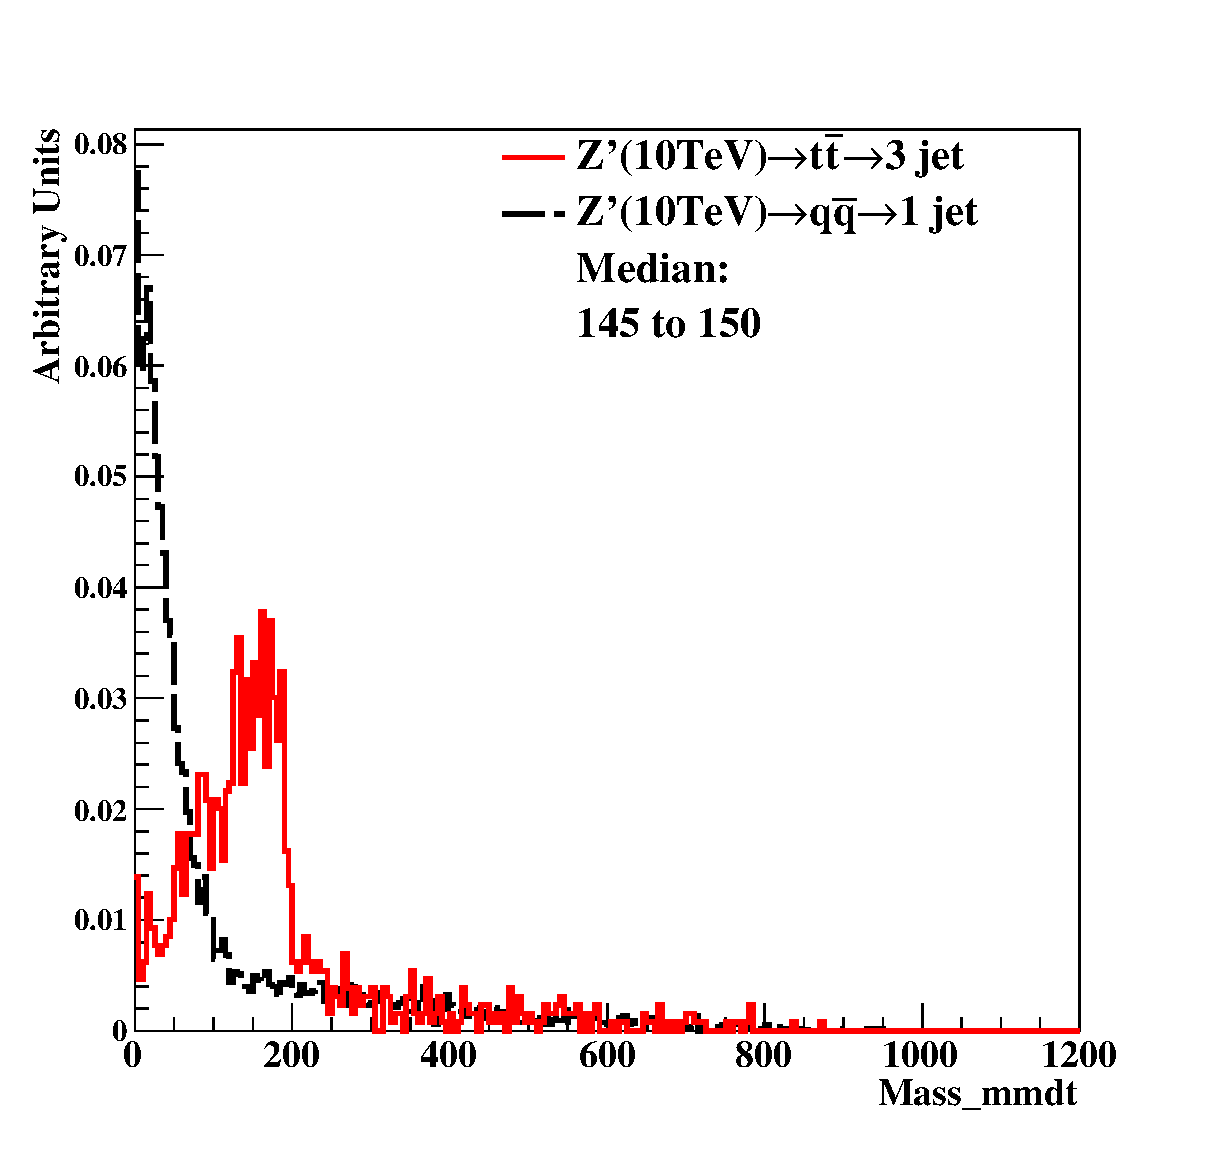
\includegraphics[width=0.22\textwidth]{figs/Dis_cluster_012_mass_mmdt_tt_10tev_04_tt_no_UOF.eps}
   }
   \subfigure[20TeV at 1$\times$1(cm$\times$cm) in cluster] {
   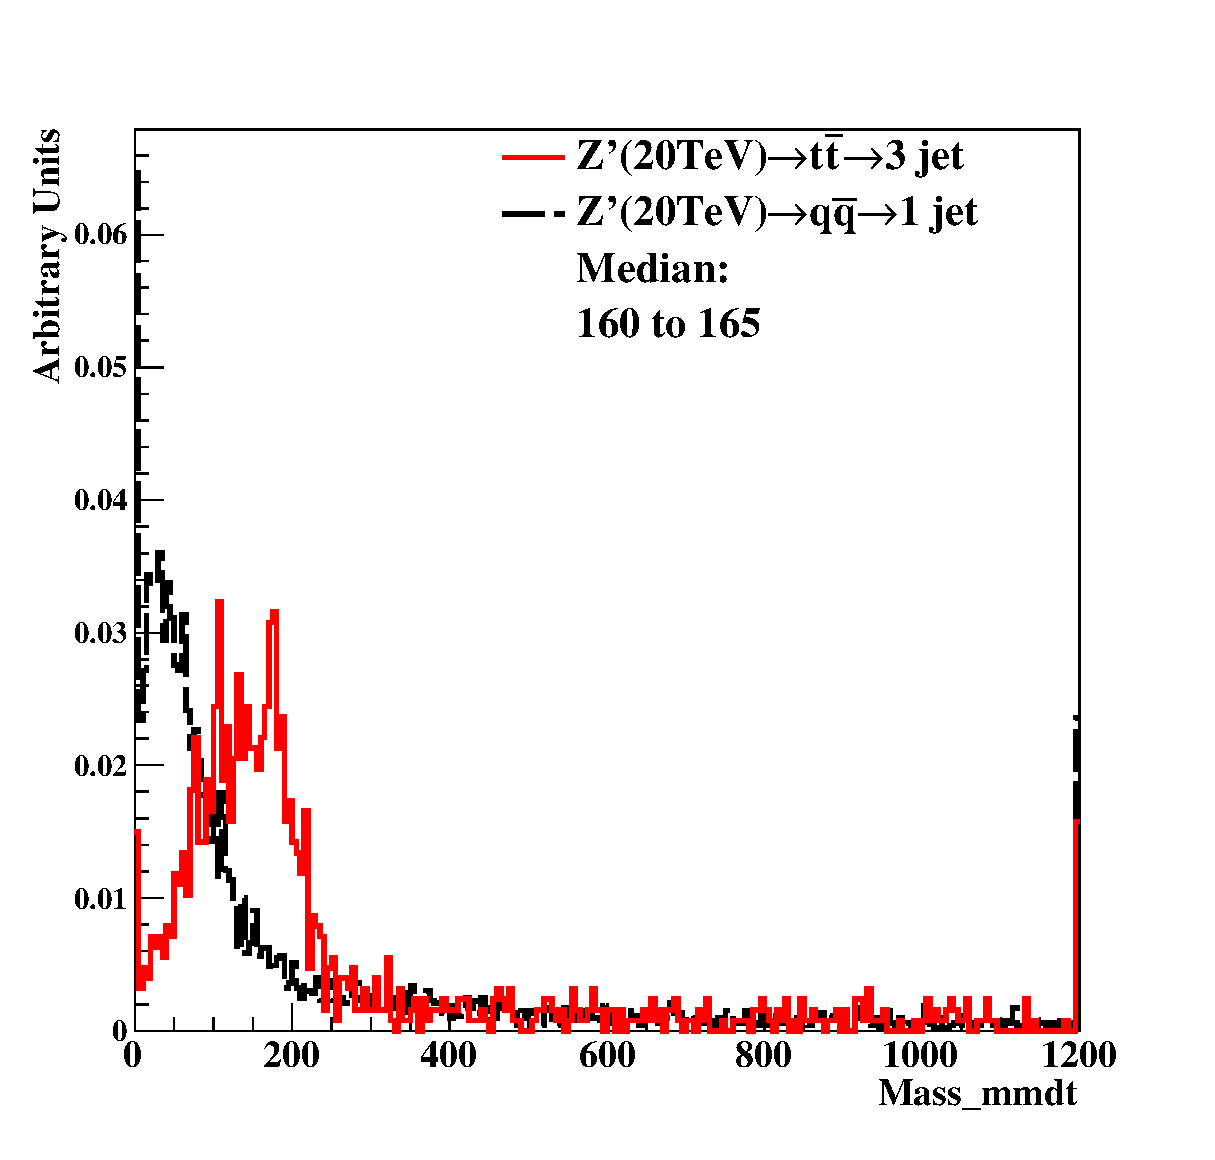
\includegraphics[width=0.22\textwidth]{figs/Dis_cluster_012_mass_mmdt_tt_20tev_04_tt_no_UOF.eps}\hfill
   }
      \subfigure[40TeV at 1$\times$1(cm$\times$cm) in cluster] {
   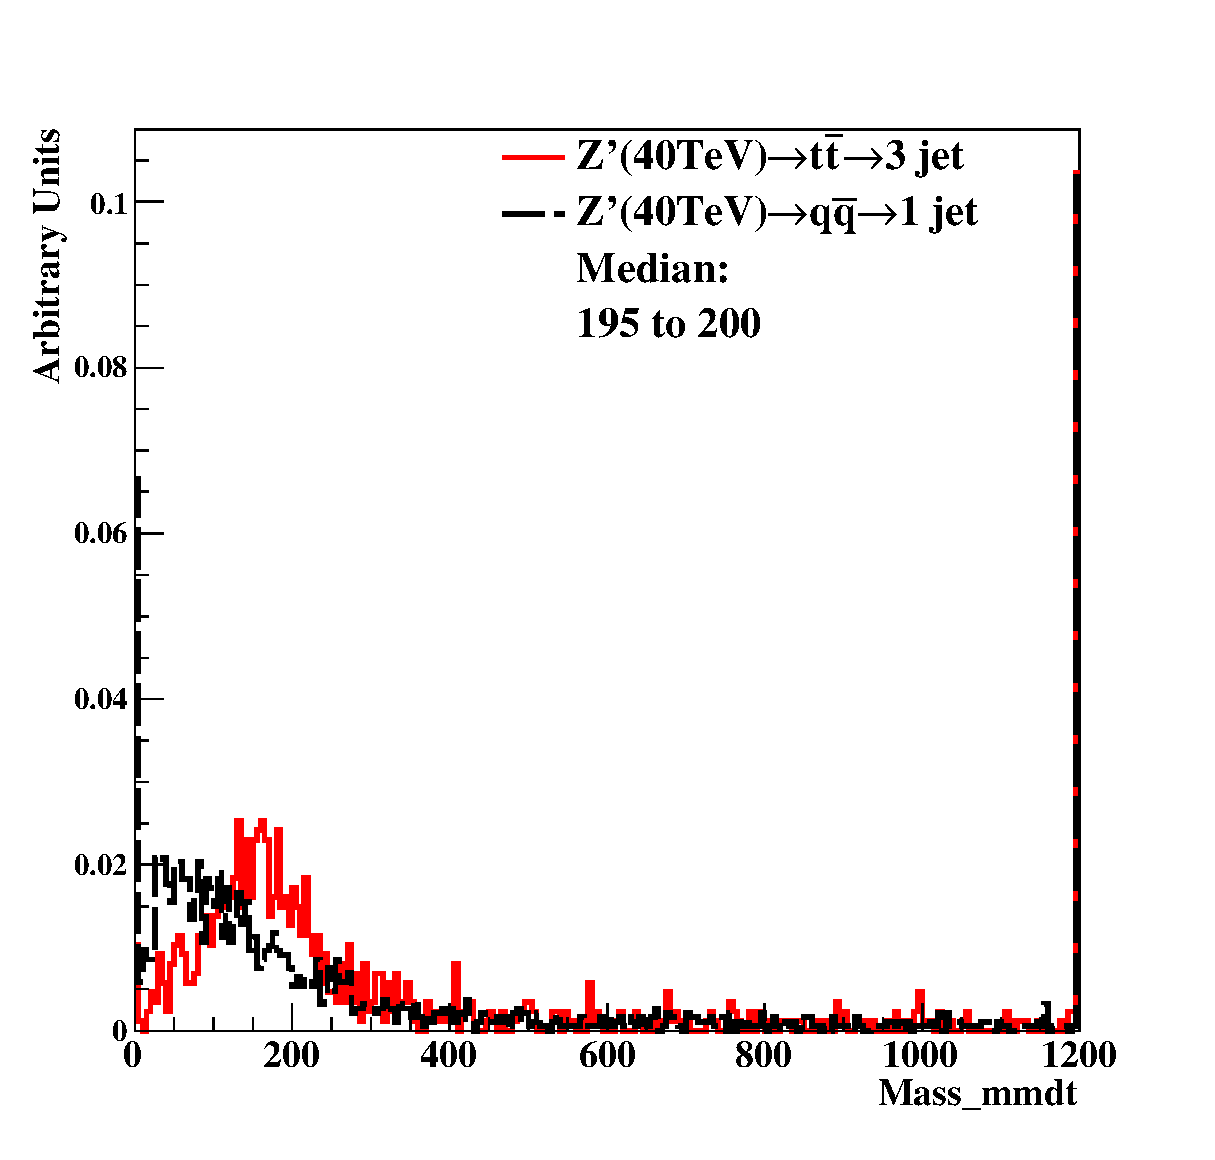
\includegraphics[width=0.22\textwidth]{figs/Dis_cluster_012_mass_mmdt_tt_40tev_04_tt_no_UOF.eps}
   }
\end{center}
\caption{Distributions of mass soft drop at $\beta$=0, signal=tt, in 5,10TeV energy of collision  in different detector sizes. Cell Size in 20$\times$20, 5$\times$5, and 1$\times$1(cm$\times$cm) are shown here.}
\label{fig:cluster_tau21_tau32}
\end{figure}


\begin{figure}
\begin{center}
  \subfigure[Central at Median($20\times20$=,$5\times5$=,$1\times1$=) change width in cluster at 5TeV] {
  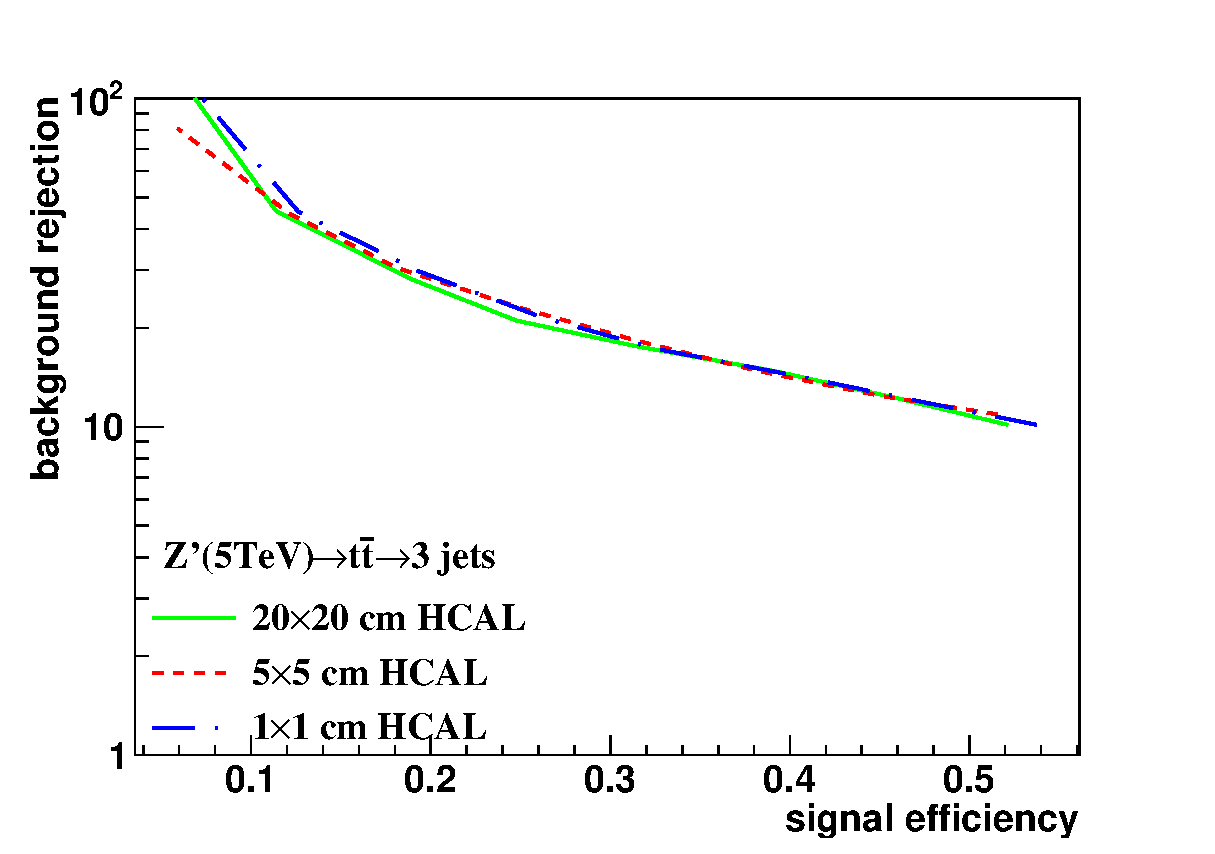
\includegraphics[width=0.43\textwidth]{figs/A_Cluster_mass_mmdt_5tev_eff_1_central_fix_tt_qq_log_no_UOF.eps}
  }
  \subfigure[Central at Median($20\times20$=,$5\times5$=,$1\times1$=) change width in cluster at 10TeV] {
  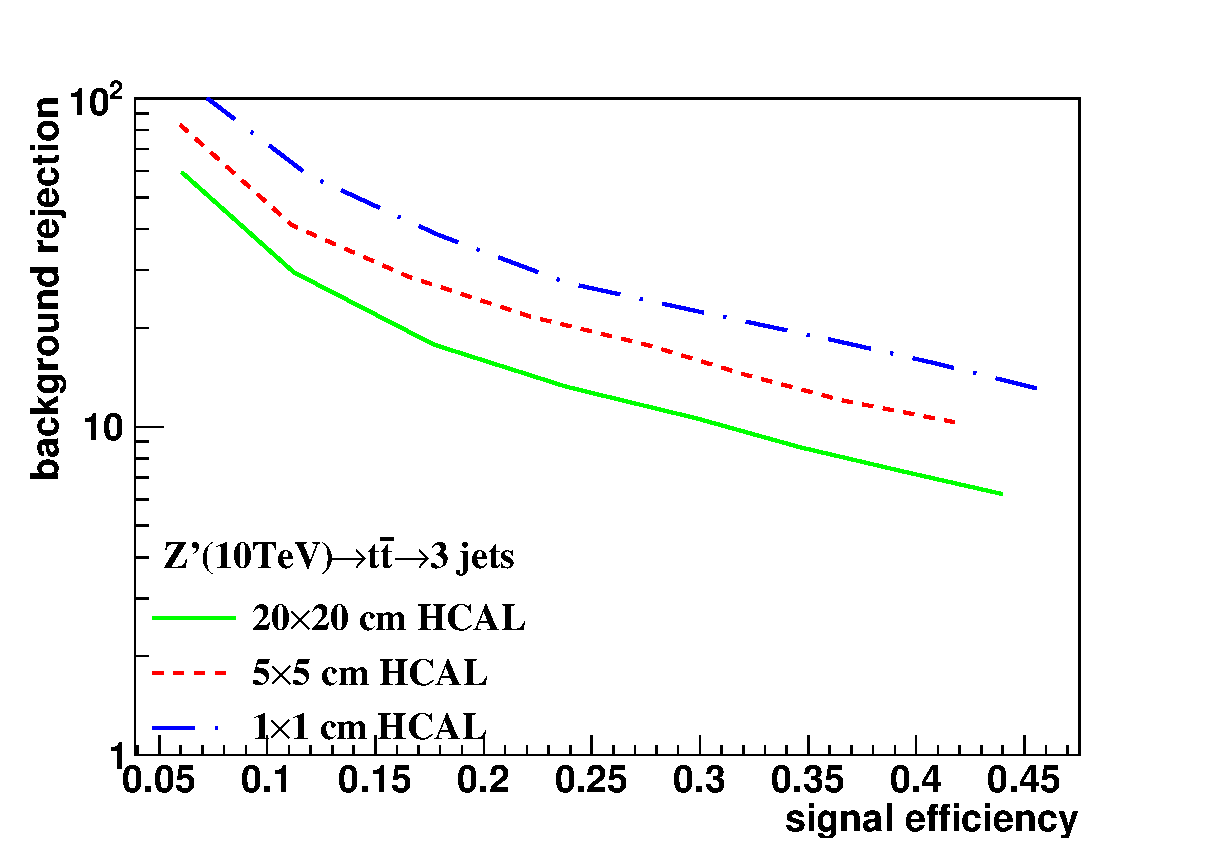
\includegraphics[width=0.43\textwidth]{figs/A_Cluster_mass_mmdt_10tev_eff_1_central_fix_tt_qq_log_no_UOF.eps}
  }
 \subfigure[Central at Median($20\times20$=,$5\times5$=,$1\times1$=) change width in cluster at 20TeV] {
 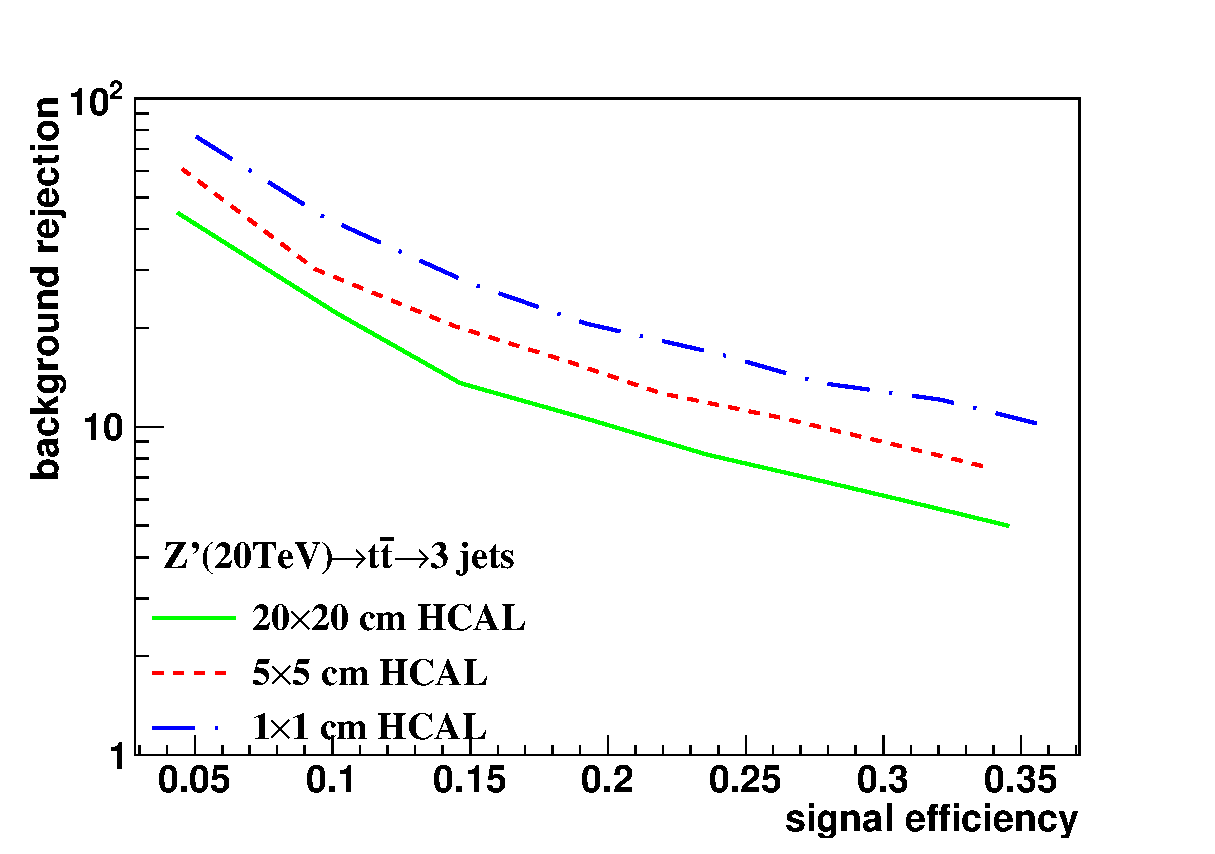
\includegraphics[width=0.43\textwidth]{figs/A_Cluster_mass_mmdt_20tev_eff_1_central_fix_tt_qq_log_no_UOF.eps}
 }
 \subfigure[Central at Median($20\times20$=,$5\times5$=,$1\times1$=) change width in cluster at 40TeV] {
 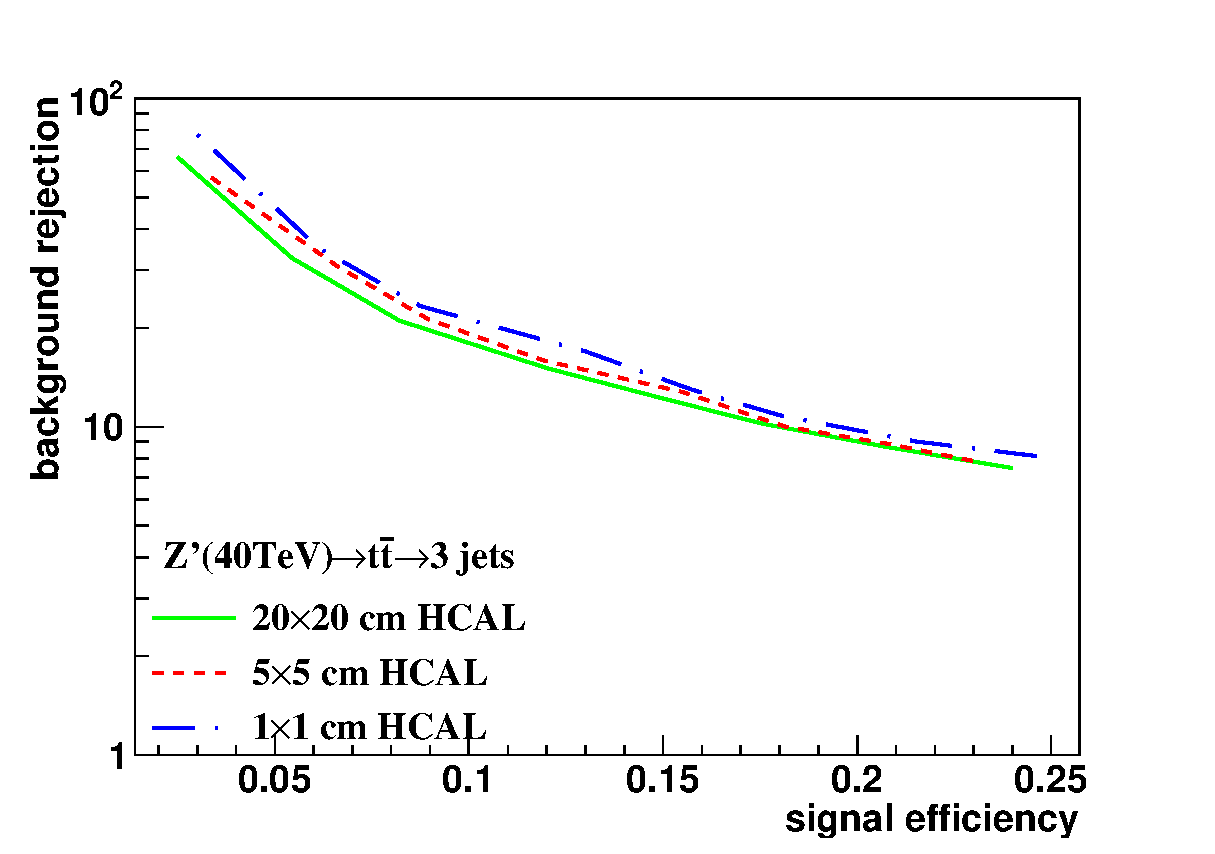
\includegraphics[width=0.43\textwidth]{figs/A_Cluster_mass_mmdt_40tev_eff_1_central_fix_tt_qq_log_no_UOF.eps}
 }
\end{center}
\caption{study of "fix central and change width" in mass soft drop at $\beta$=0, signal=tt, in 5, 10, 20, 40TeV energy of collision  in different detector sizes. Cell Size in 20$\times$20, 5$\times$5, and 1$\times$1(cm$\times$cm) are shown in each picture.}
\label{fig:cluster_tau21_tau32}
\end{figure}



\begin{figure}
\begin{center}
   \subfigure[5TeV at 20$\times$20(cm$\times$cm) in cluster] {
   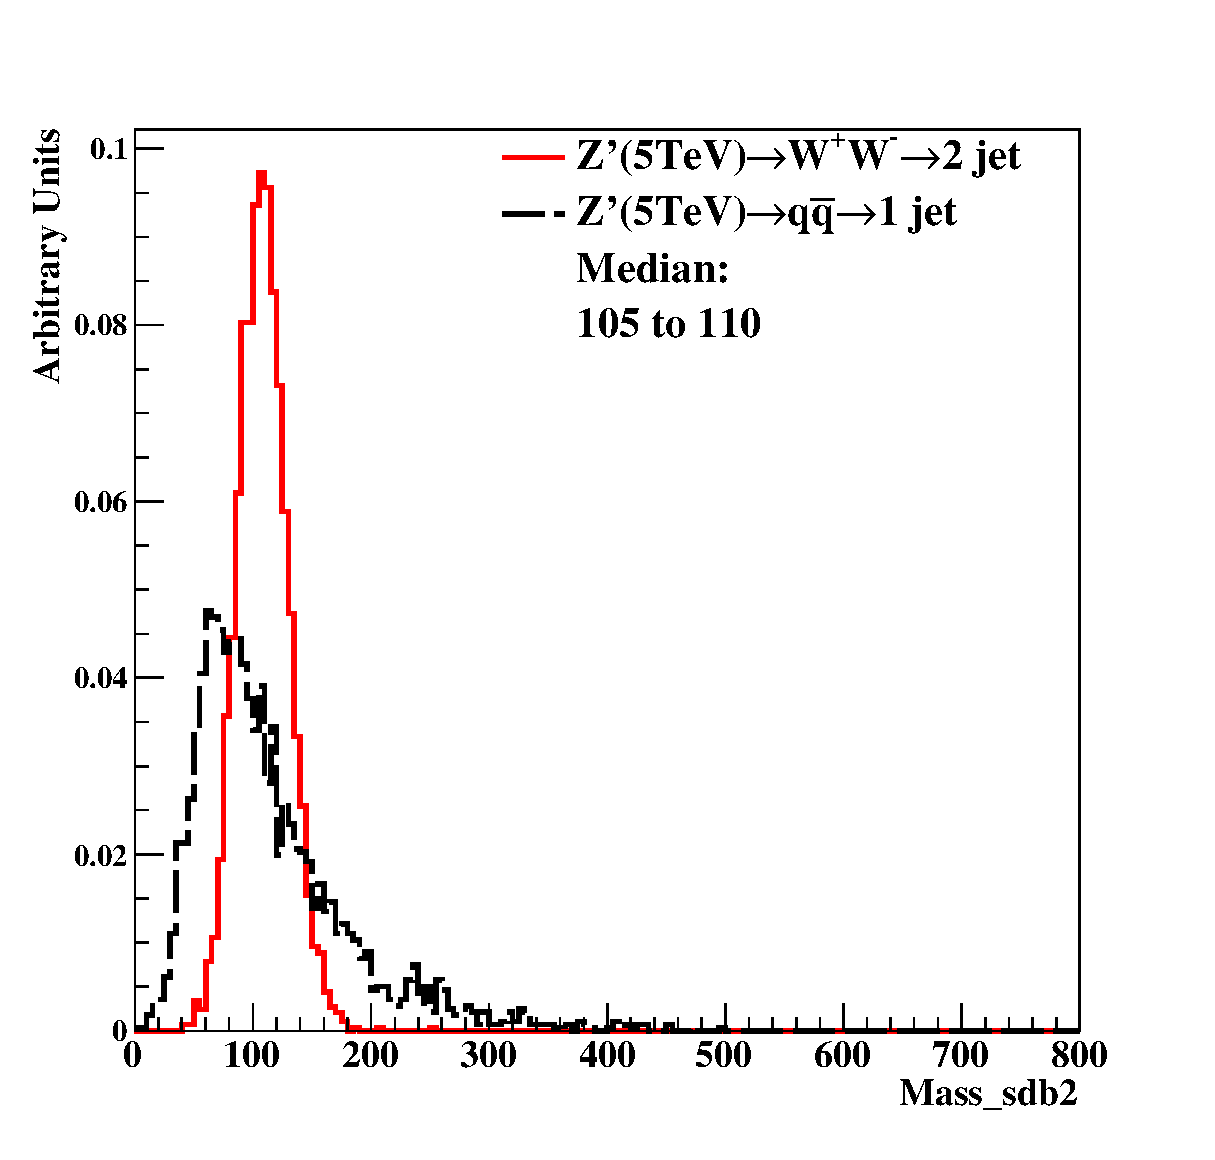
\includegraphics[width=0.22\textwidth]{figs/Dis_cluster_010_mass_sdb2_ww_5tev_04_800_no_UOF.eps}
   }
      \subfigure[10TeV at 20$\times$20(cm$\times$cm) in cluster] {
   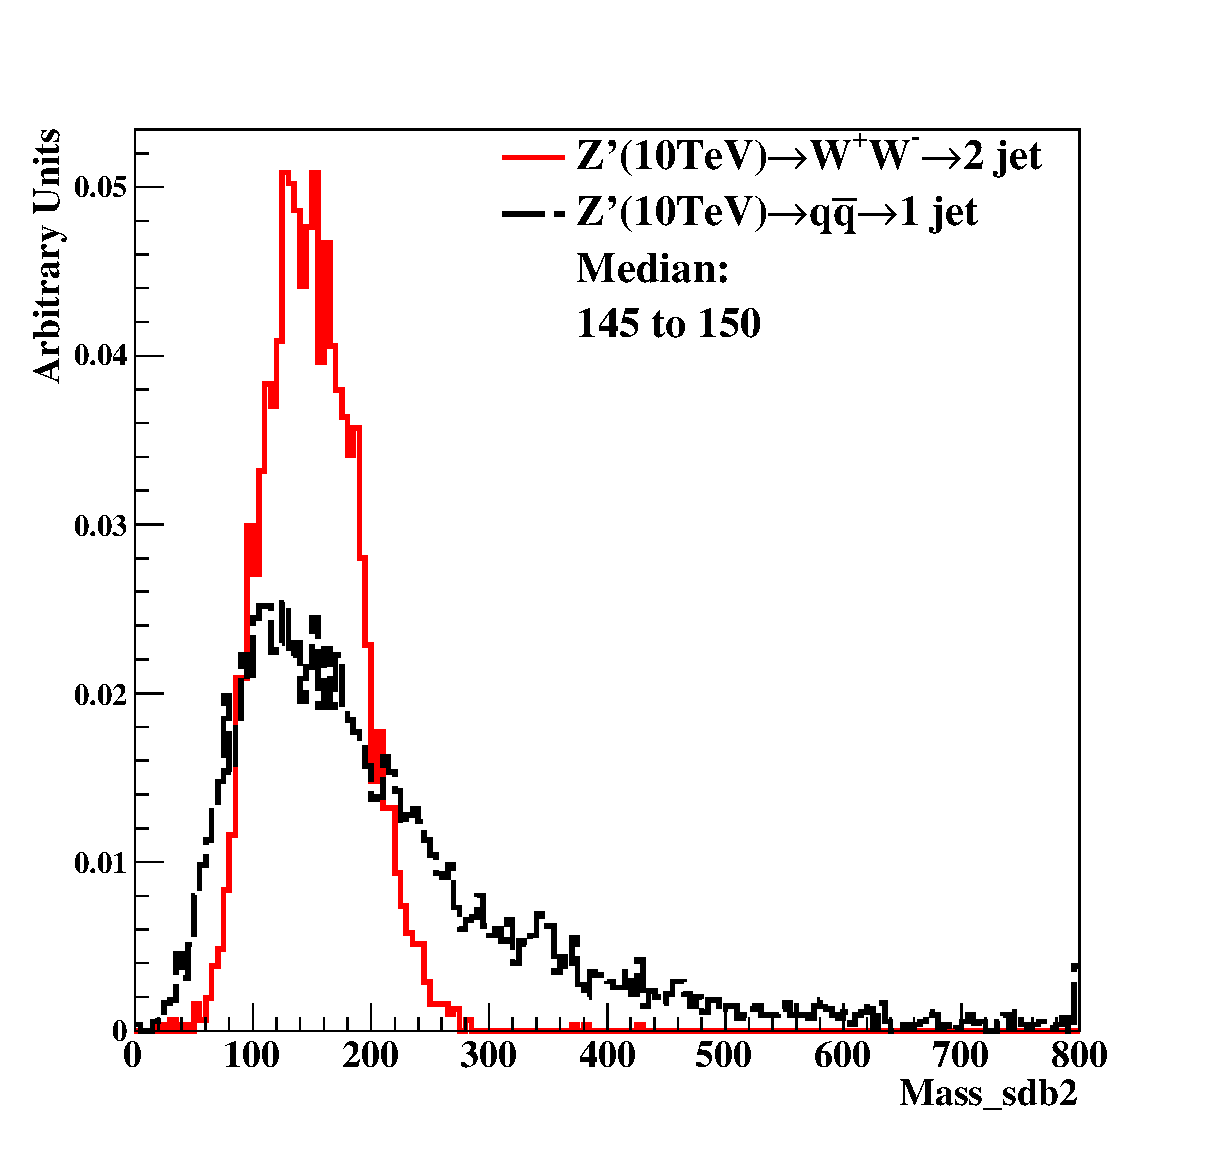
\includegraphics[width=0.22\textwidth]{figs/Dis_cluster_010_mass_sdb2_ww_10tev_04_800_no_UOF.eps}
   }
   \subfigure[20TeV at 20$\times$20(cm$\times$cm) in cluster] {
   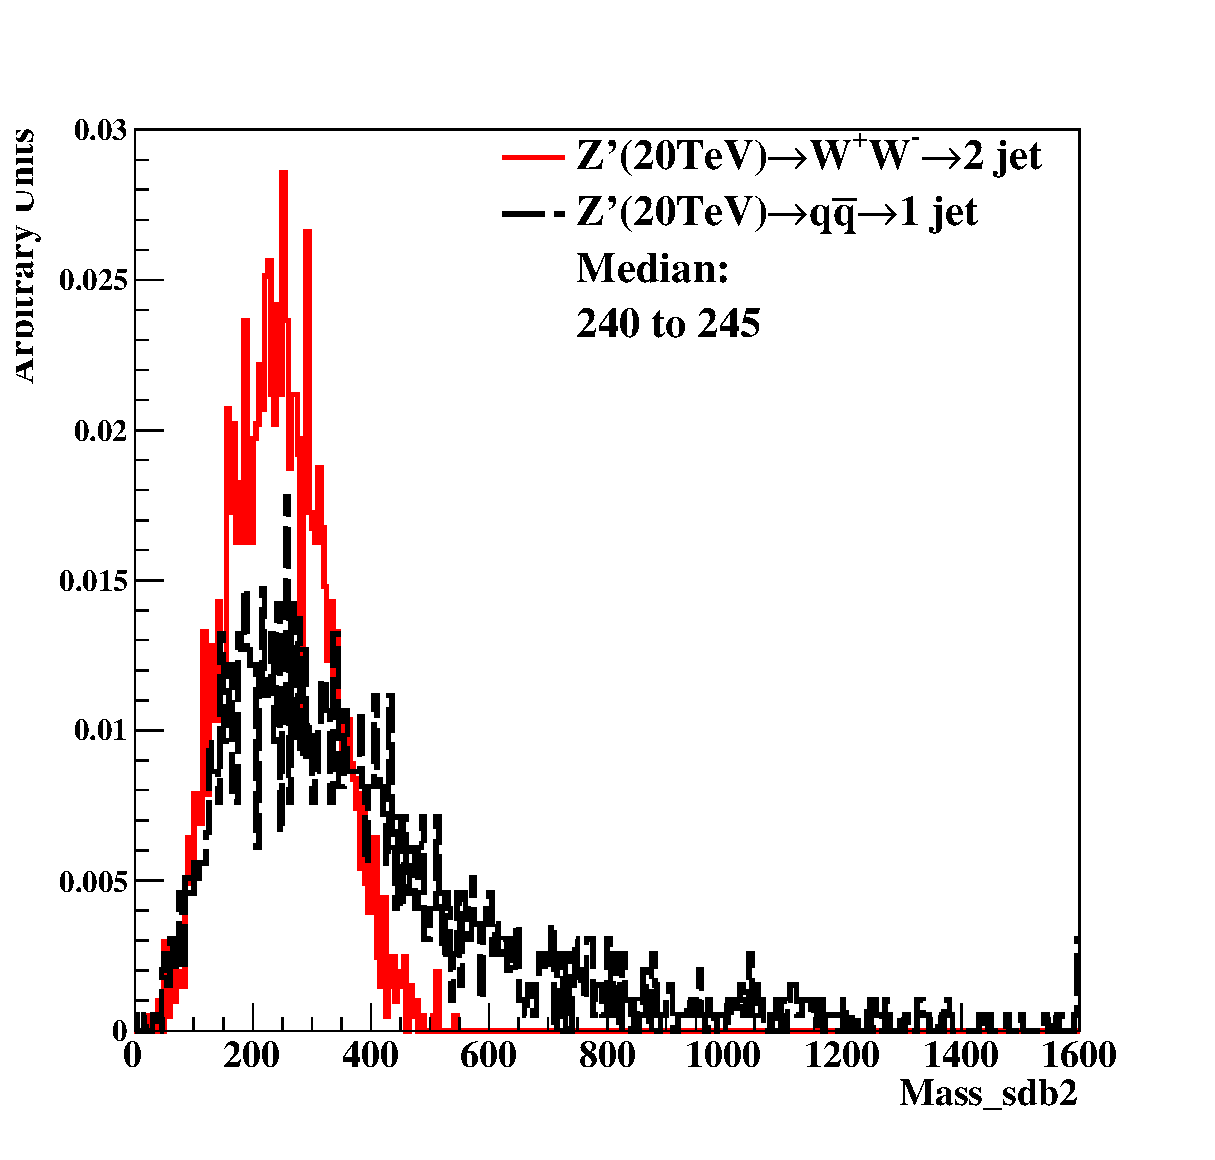
\includegraphics[width=0.22\textwidth]{figs/Dis_cluster_010_mass_sdb2_ww_20tev_04_1600_no_UOF.eps}
   }
    \subfigure[40TeV at 20$\times$20(cm$\times$cm) in cluster] {
   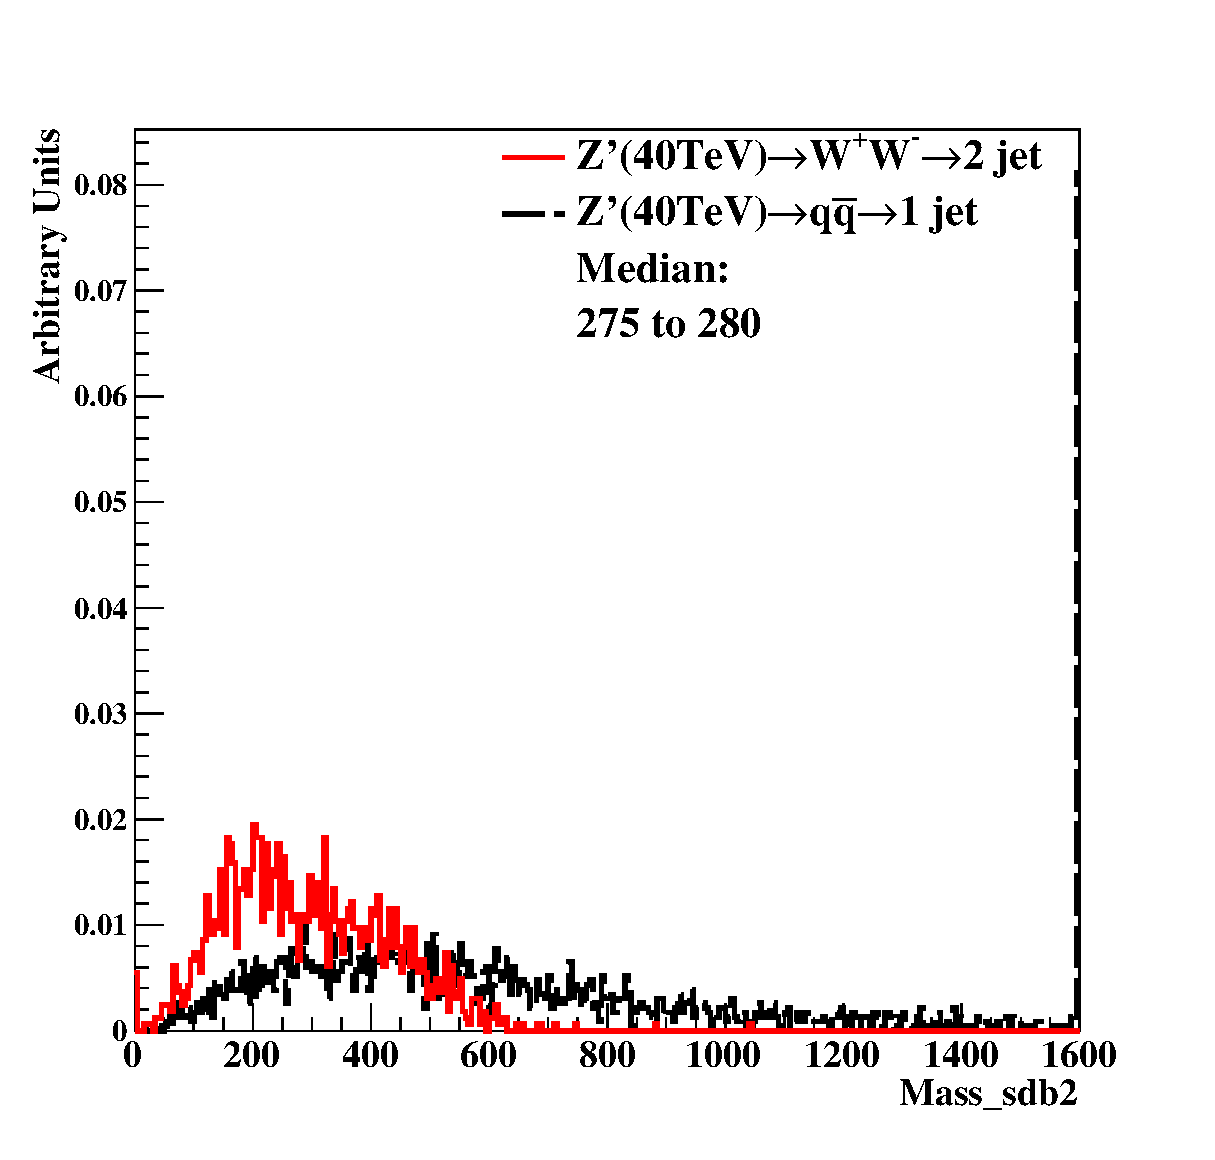
\includegraphics[width=0.22\textwidth]{figs/Dis_cluster_010_mass_sdb2_ww_40tev_04_1600_no_UOF.eps}
   }
   \subfigure[5TeV at 5$\times$5(cm$\times$cm) in cluster] {
   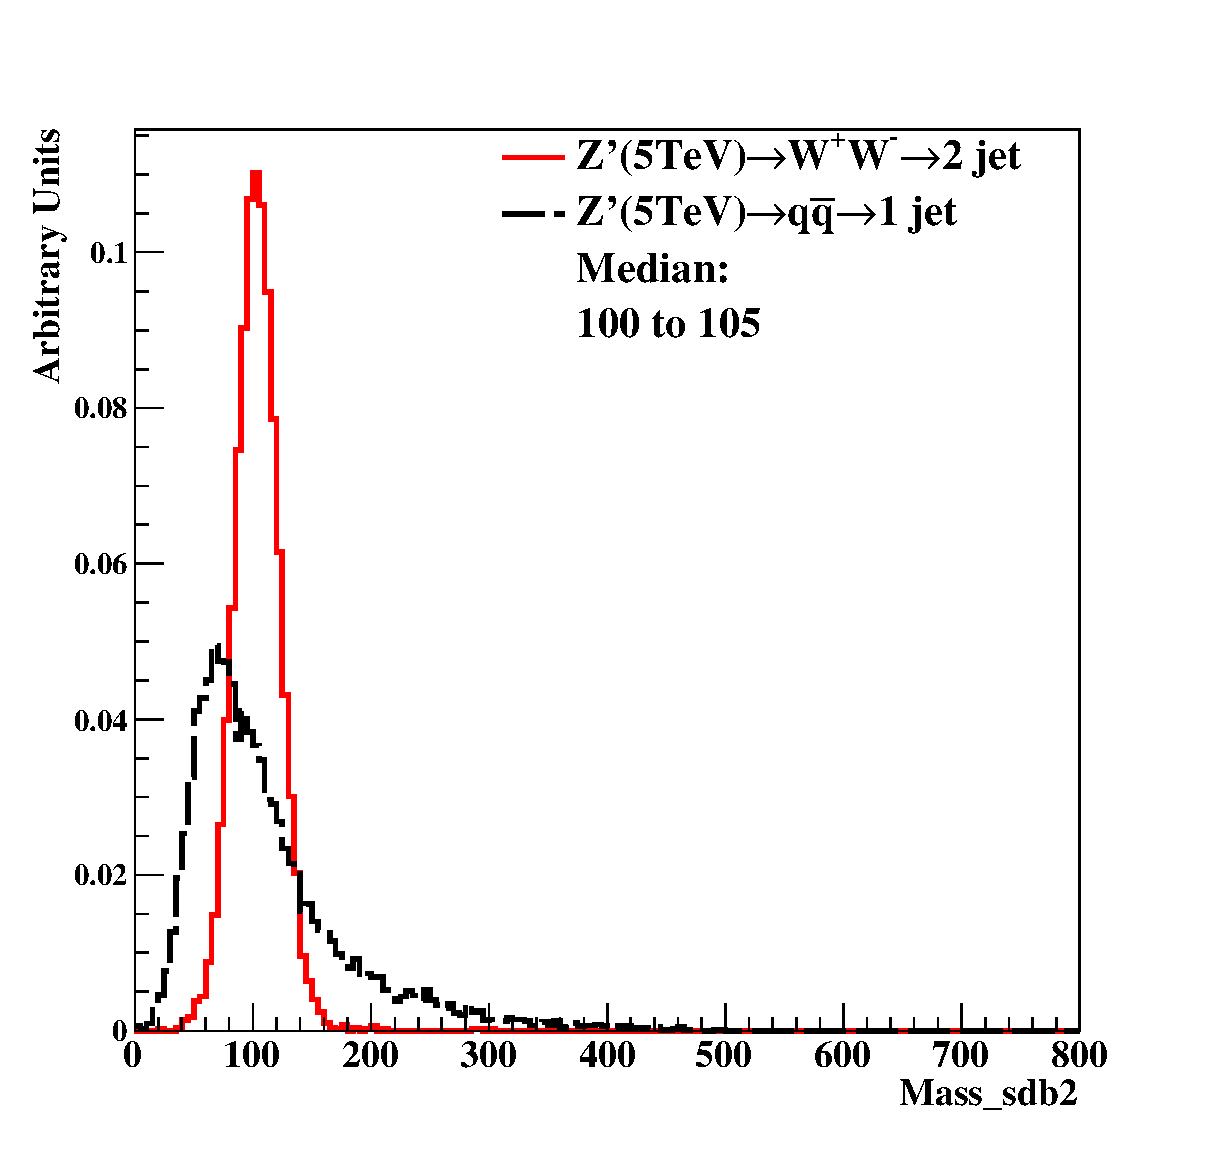
\includegraphics[width=0.22\textwidth]{figs/Dis_cluster_009_mass_sdb2_ww_5tev_04_800_no_UOF.eps}
   }
   \subfigure[10TeV at 5$\times$5(cm$\times$cm) in cluster] {
   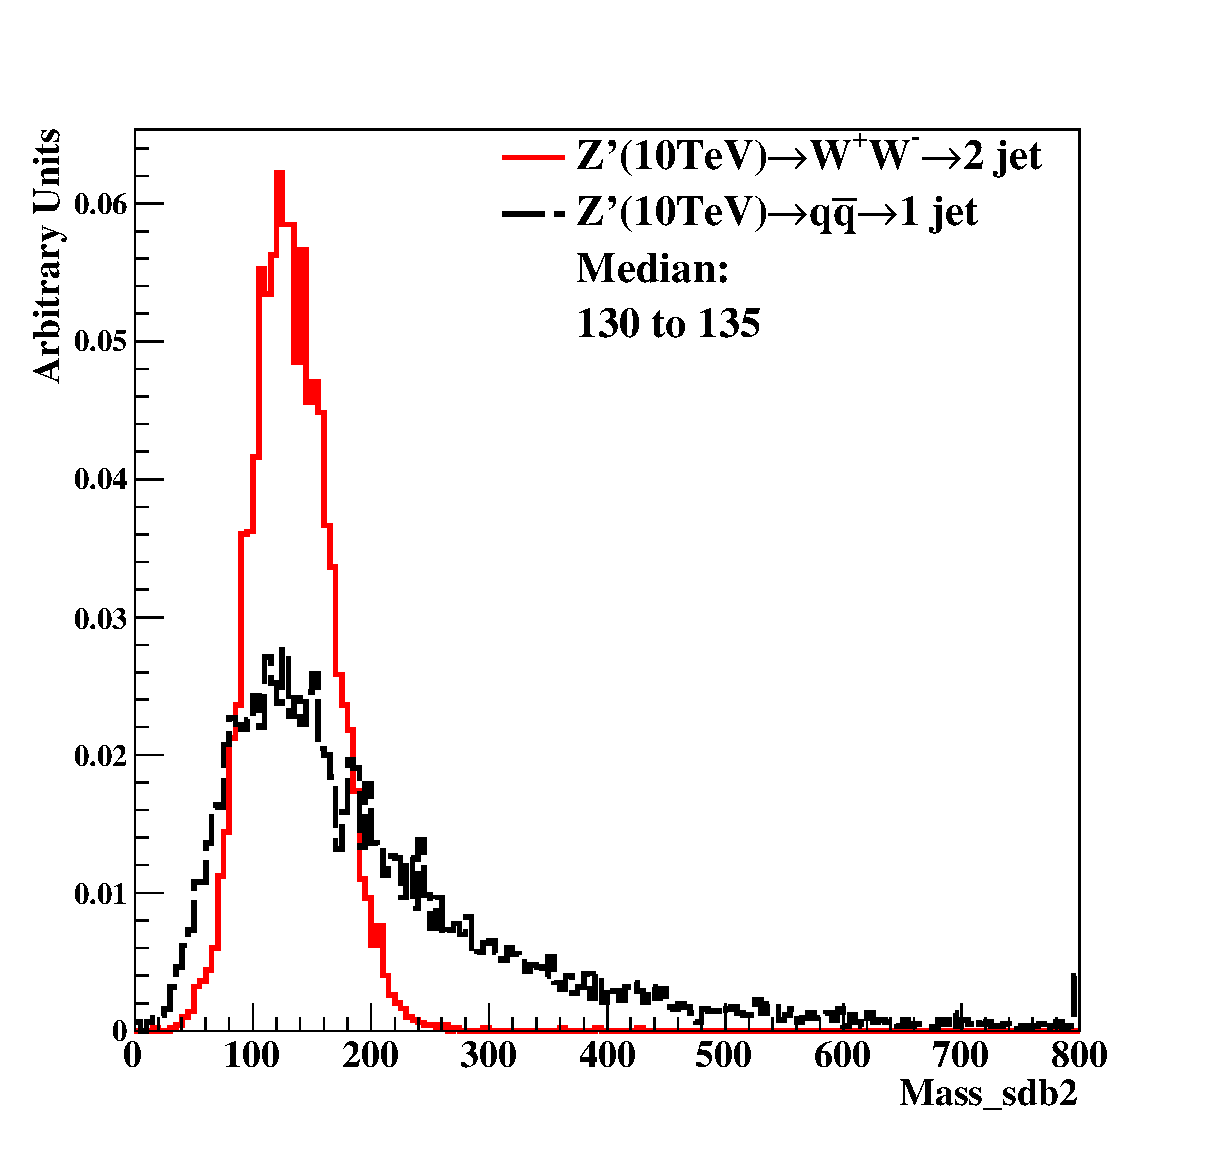
\includegraphics[width=0.22\textwidth]{figs/Dis_cluster_009_mass_sdb2_ww_10tev_04_800_no_UOF.eps}
   }
    \subfigure[20TeV at 5$\times$5(cm$\times$cm) in cluster] {
   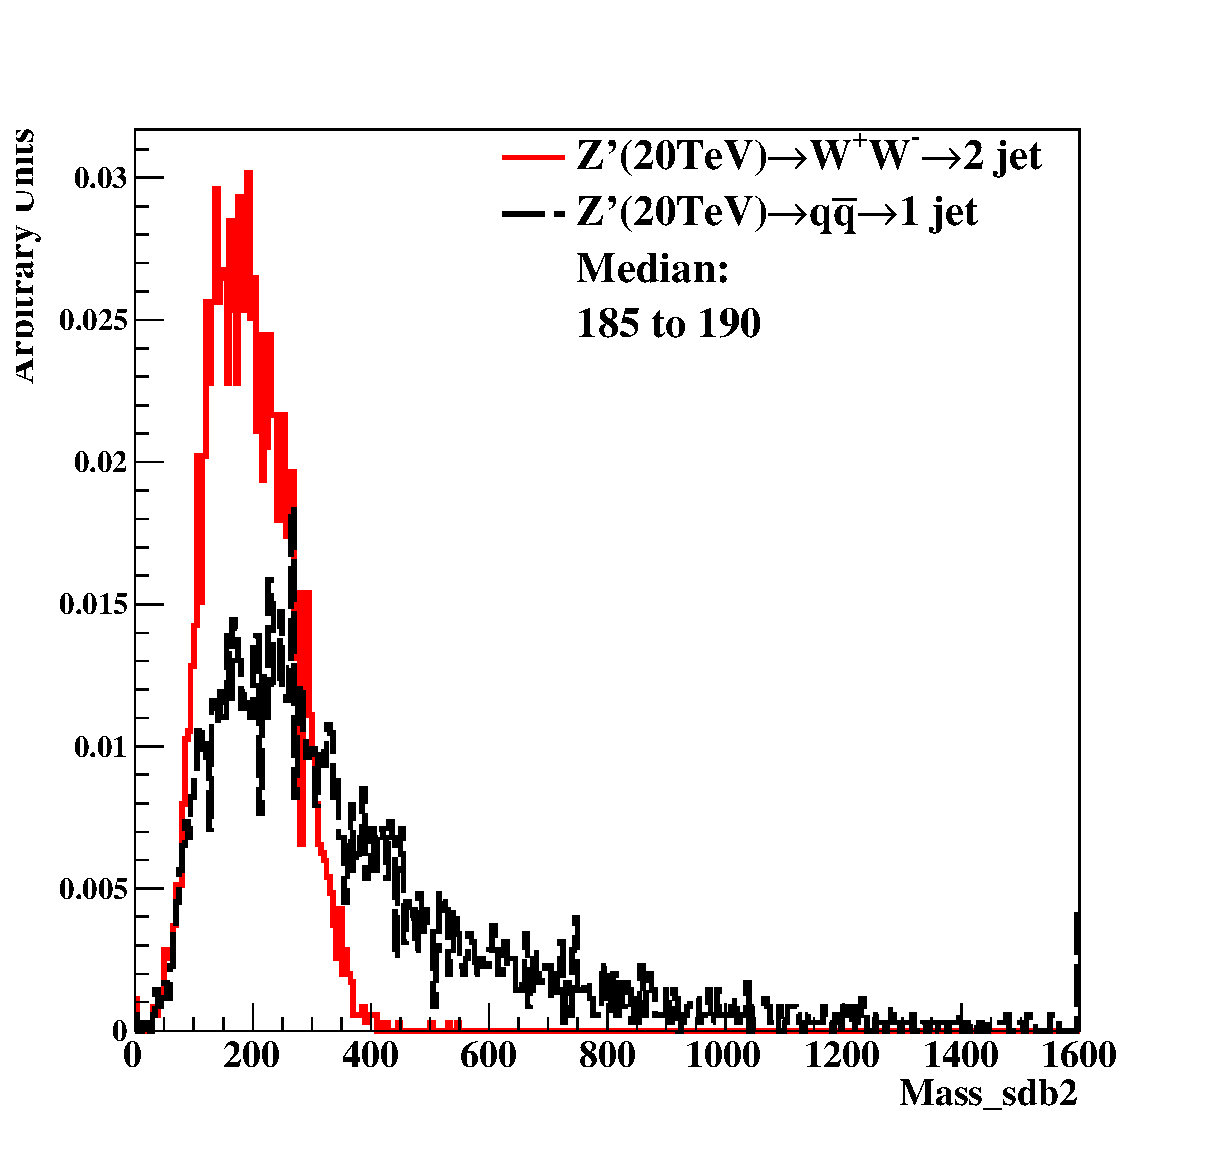
\includegraphics[width=0.22\textwidth]{figs/Dis_cluster_009_mass_sdb2_ww_20tev_04_1600_no_UOF.eps}\hfill
   }
      \subfigure[40TeV at 5$\times$5(cm$\times$cm) in cluster] {
   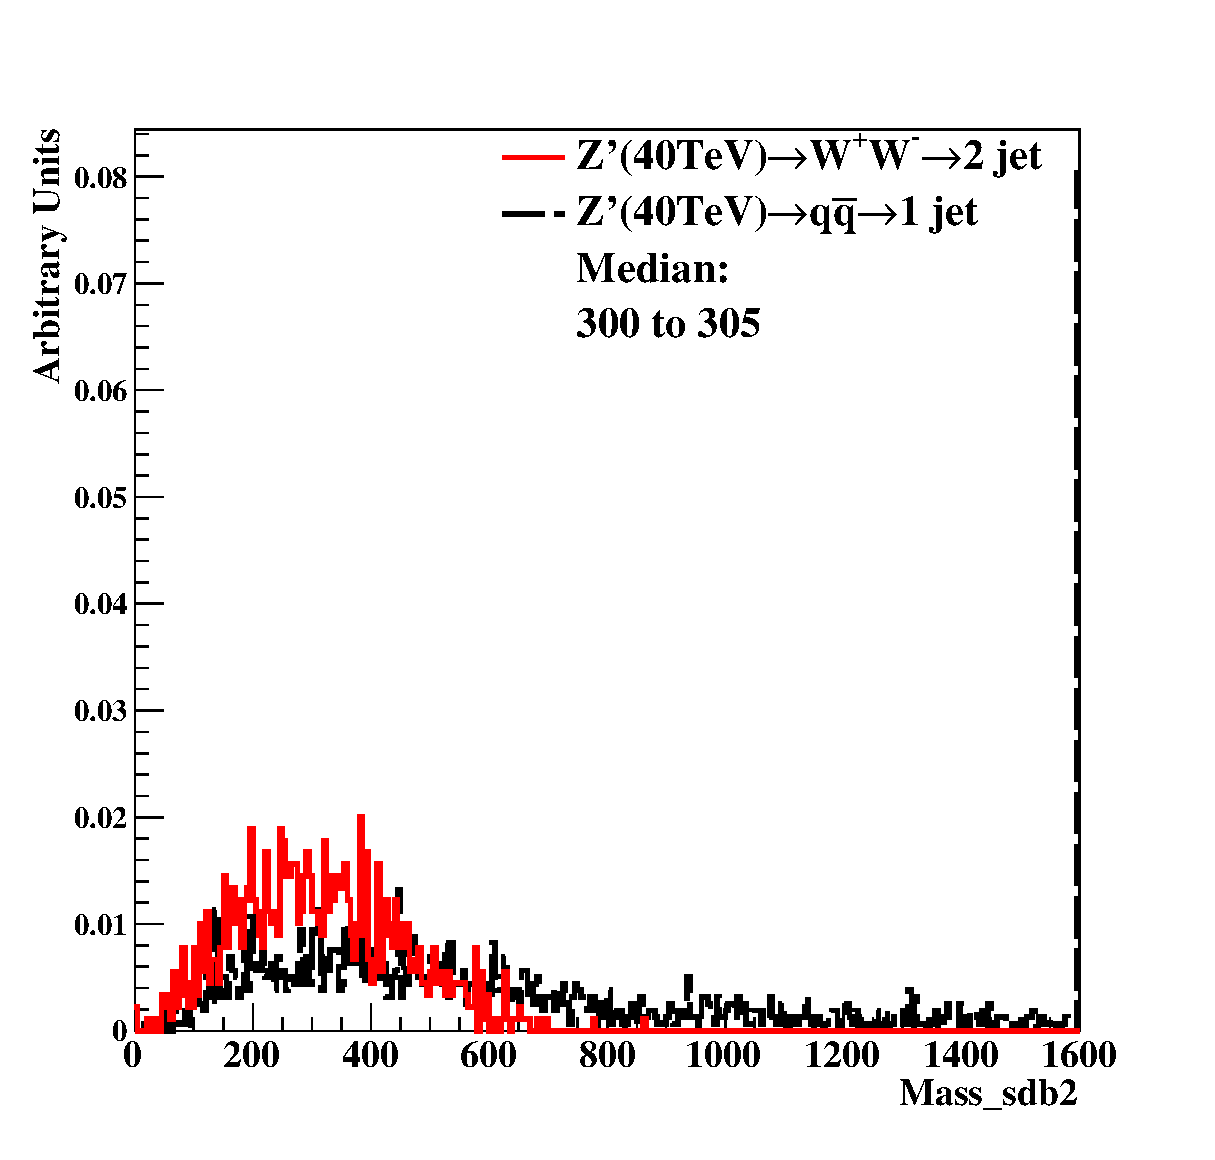
\includegraphics[width=0.22\textwidth]{figs/Dis_cluster_009_mass_sdb2_ww_40tev_04_1600_no_UOF.eps}\hfill
   }
   \subfigure[5TeV at 1$\times$1(cm$\times$cm) in cluster] {
   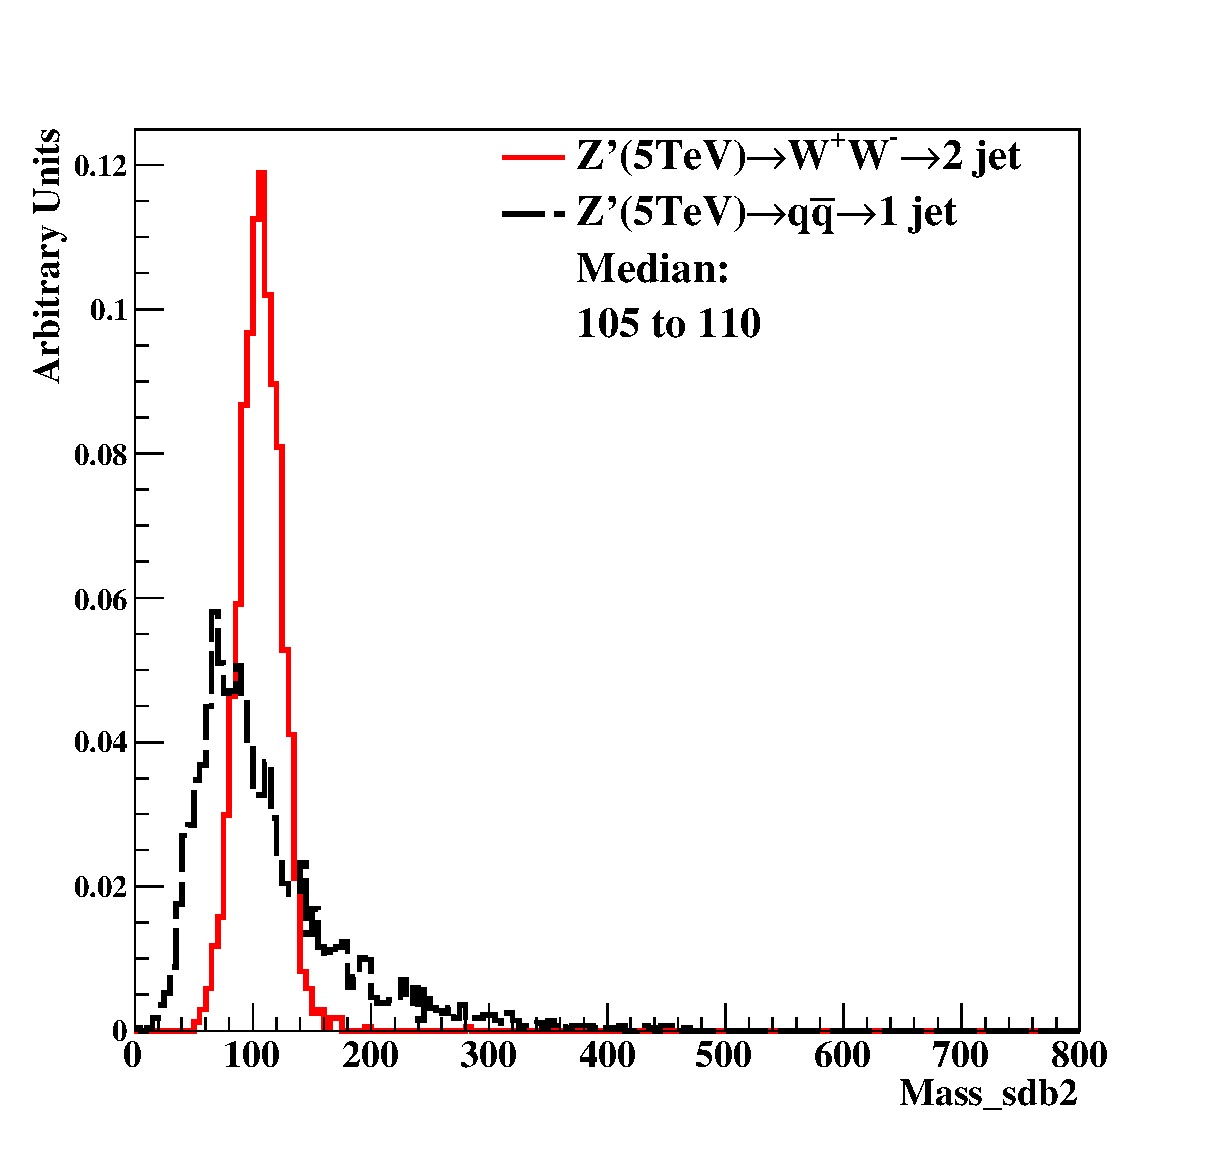
\includegraphics[width=0.22\textwidth]{figs/Dis_cluster_012_mass_sdb2_ww_5tev_04_800_no_UOF.eps}\hfill
   }
    \subfigure[10TeV at 1$\times$1(cm$\times$cm) in cluster] {
   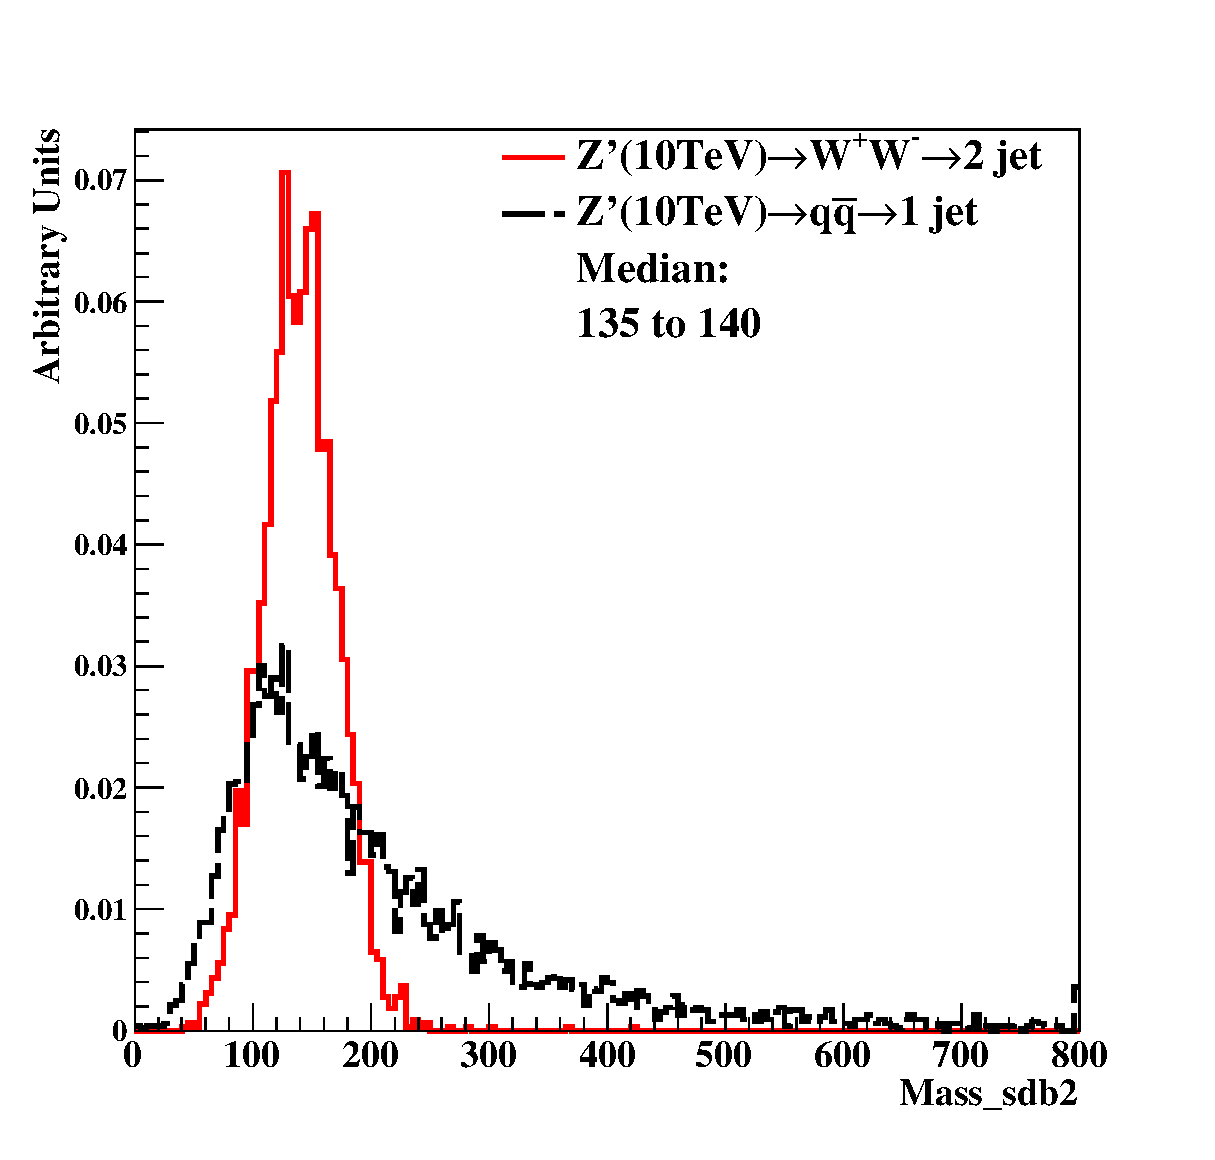
\includegraphics[width=0.22\textwidth]{figs/Dis_cluster_012_mass_sdb2_ww_10tev_04_800_no_UOF.eps}
   }
   \subfigure[20TeV at 1$\times$1(cm$\times$cm) in cluster] {
   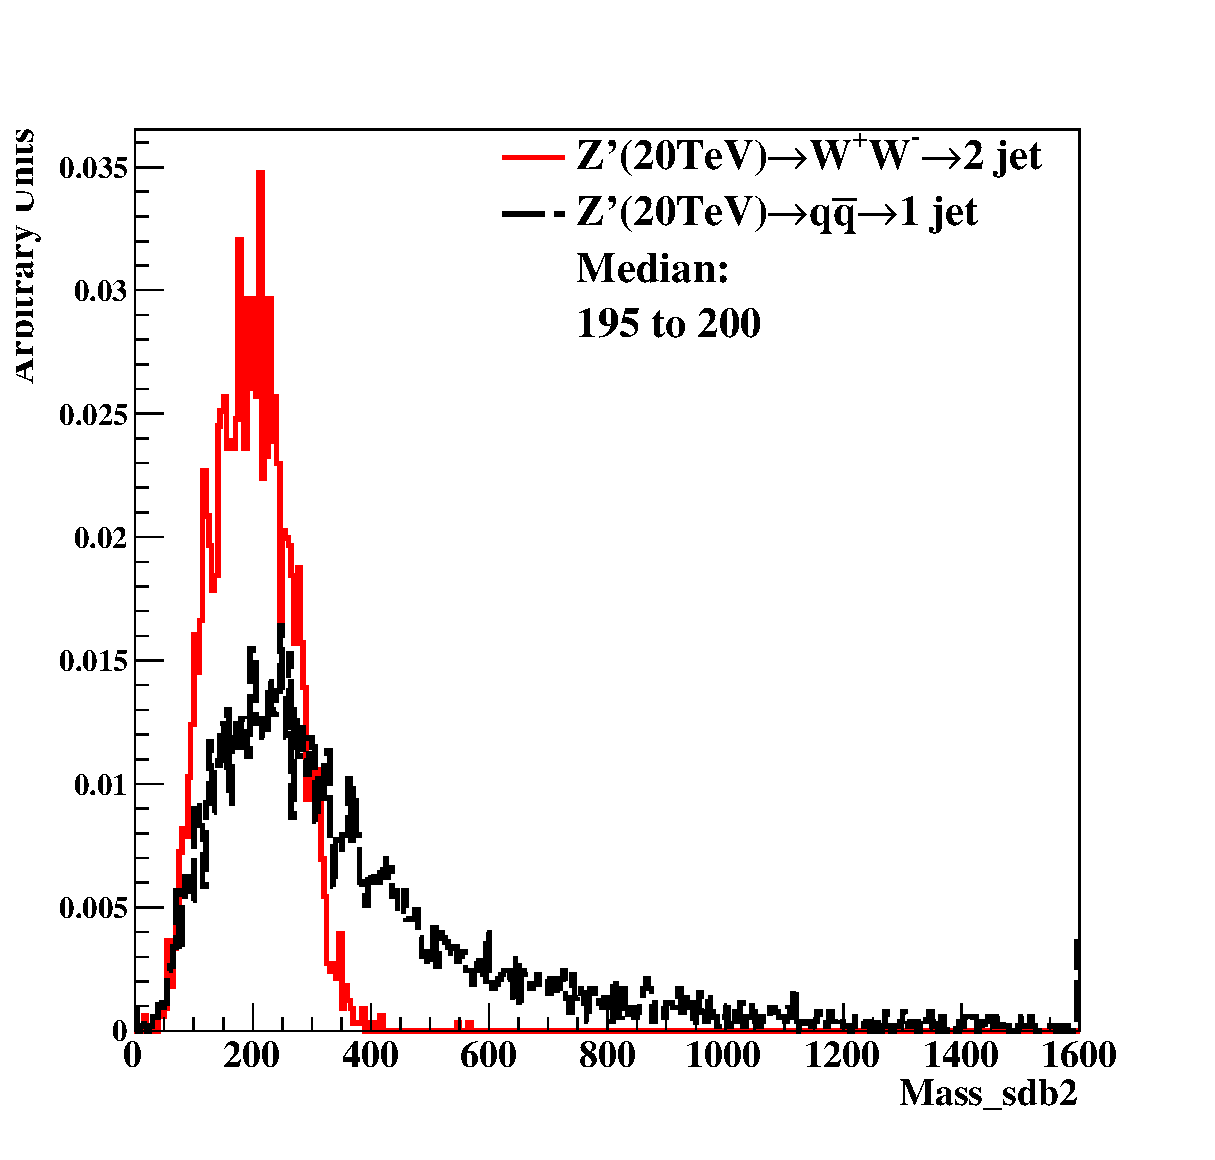
\includegraphics[width=0.22\textwidth]{figs/Dis_cluster_012_mass_sdb2_ww_20tev_04_1600_no_UOF.eps}\hfill
   }
      \subfigure[40TeV at 1$\times$1(cm$\times$cm) in cluster] {
   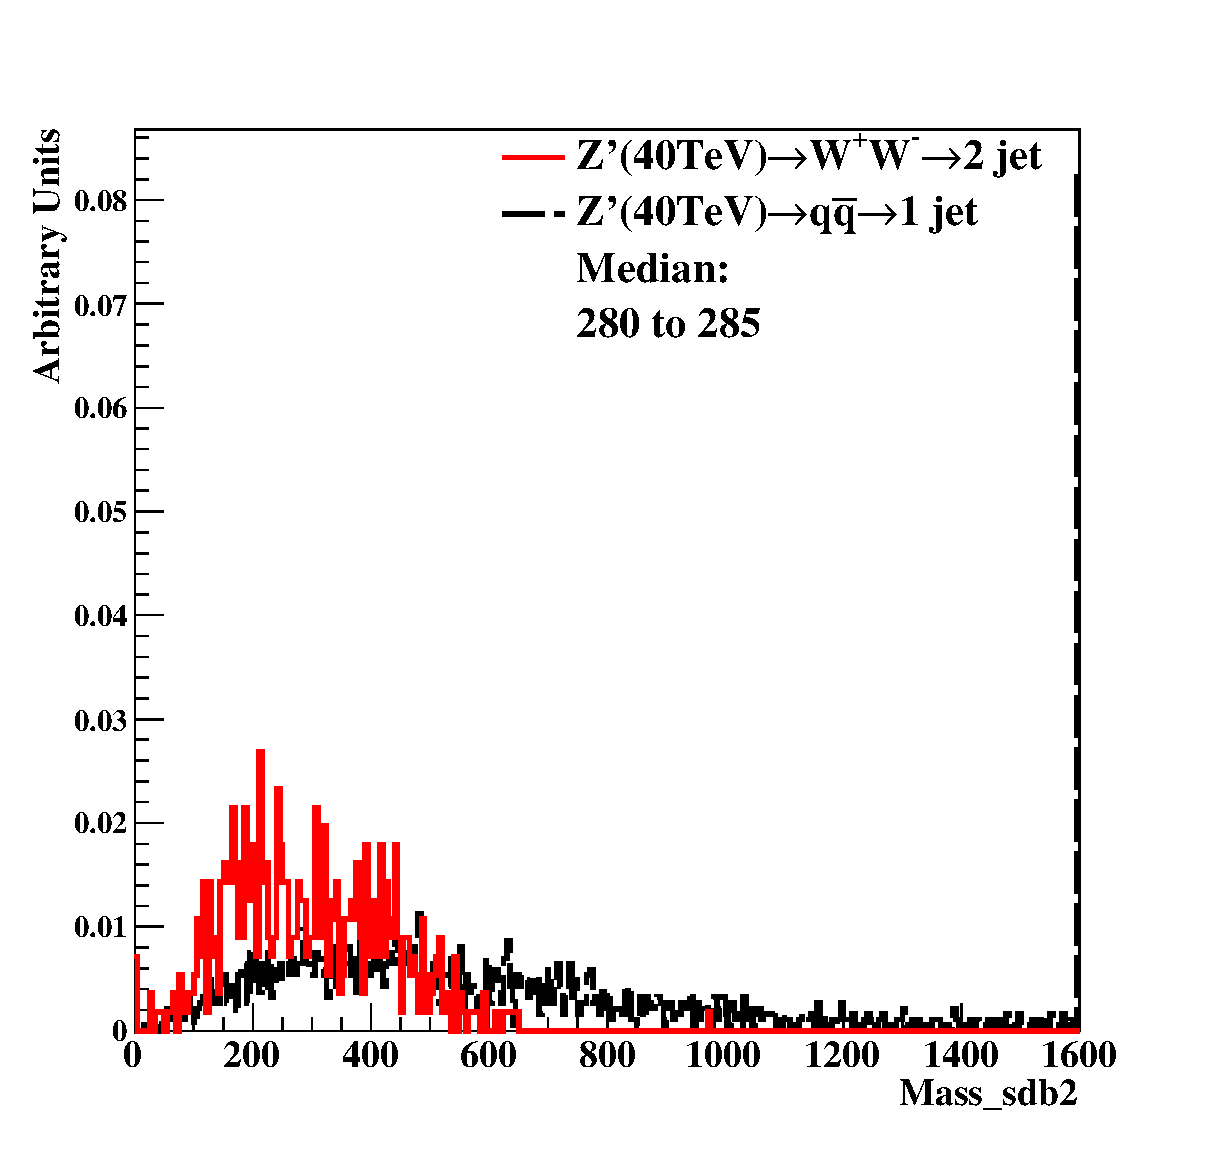
\includegraphics[width=0.22\textwidth]{figs/Dis_cluster_012_mass_sdb2_ww_40tev_04_1600_no_UOF.eps}
   }
\end{center}
\caption{Distributions of mass soft drop at $\beta$=2, signal=ww, in 5,10TeV energy of collision  in different detector sizes. Cell Size in 20$\times$20, 5$\times$5, and 1$\times$1(cm$\times$cm) are shown here.}
\label{fig:cluster_tau21_tau32}
\end{figure}


\begin{figure}
\begin{center}
  \subfigure[Central at Median($20\times20$=,$5\times5$=,$1\times1$=) change width in cluster at 5TeV] {
  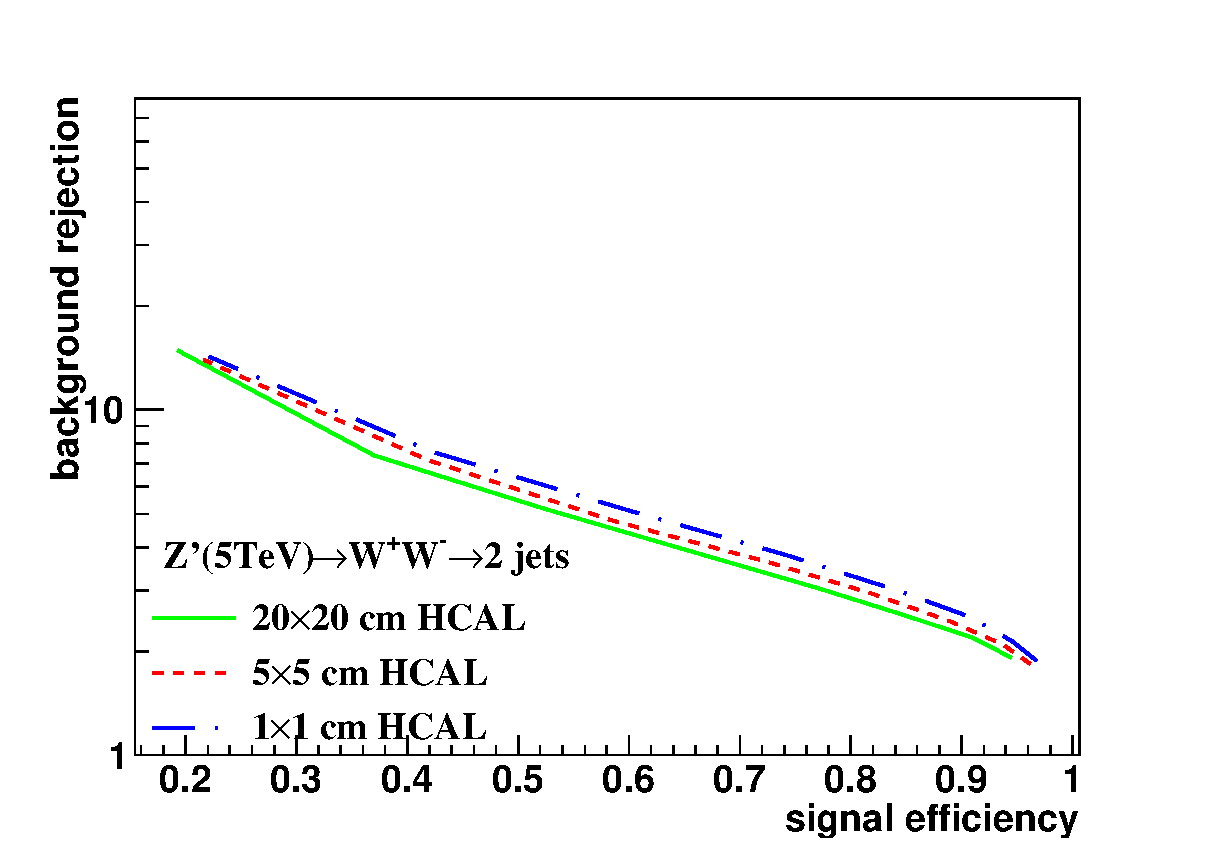
\includegraphics[width=0.43\textwidth]{figs/A_Cluster_mass_sdb2_5tev_eff_1_central_fix_ww_qq_log_no_UOF.eps}
  }
  \subfigure[Central at Median($20\times20$=,$5\times5$=,$1\times1$=) change width in cluster at 10TeV] {
  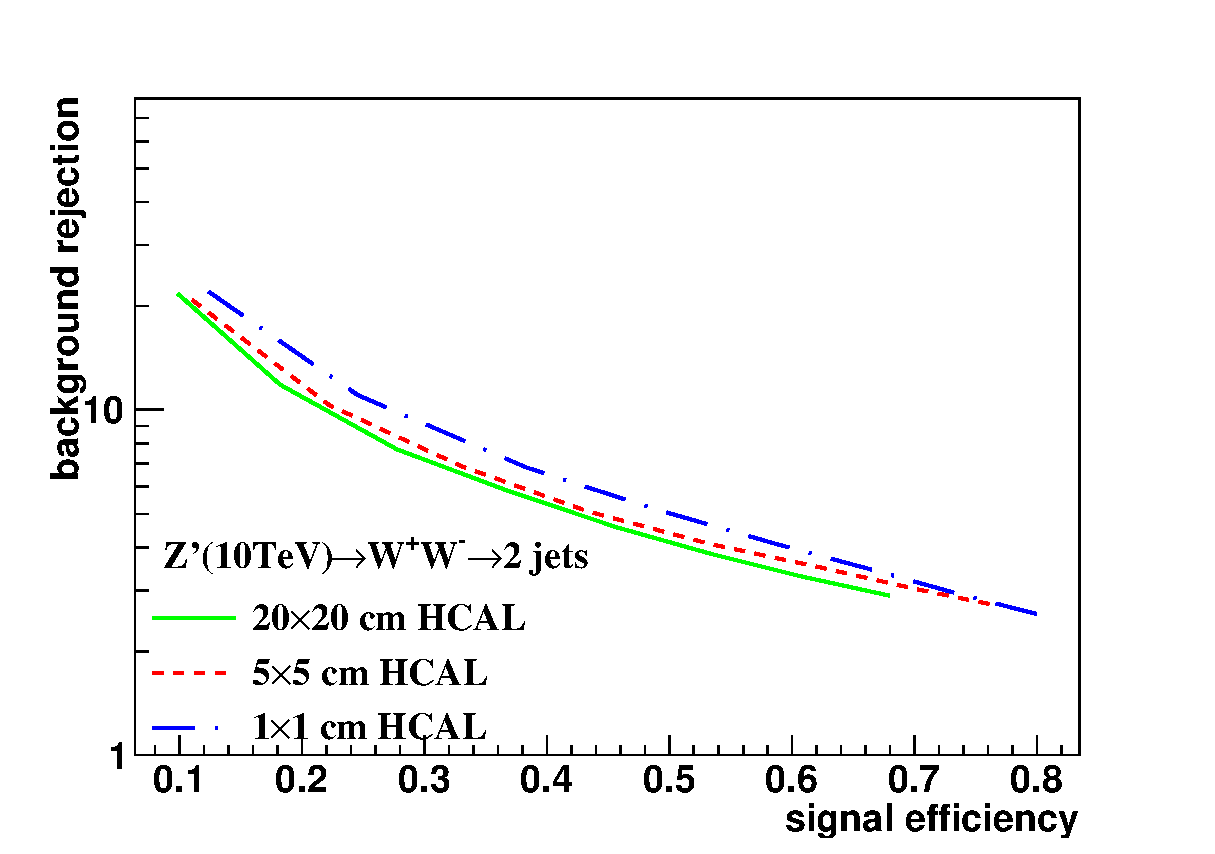
\includegraphics[width=0.43\textwidth]{figs/A_Cluster_mass_sdb2_10tev_eff_1_central_fix_ww_qq_log_no_UOF.eps}
  }
 \subfigure[Central at Median($20\times20$=,$5\times5$=,$1\times1$=) change width in cluster at 20TeV] {
 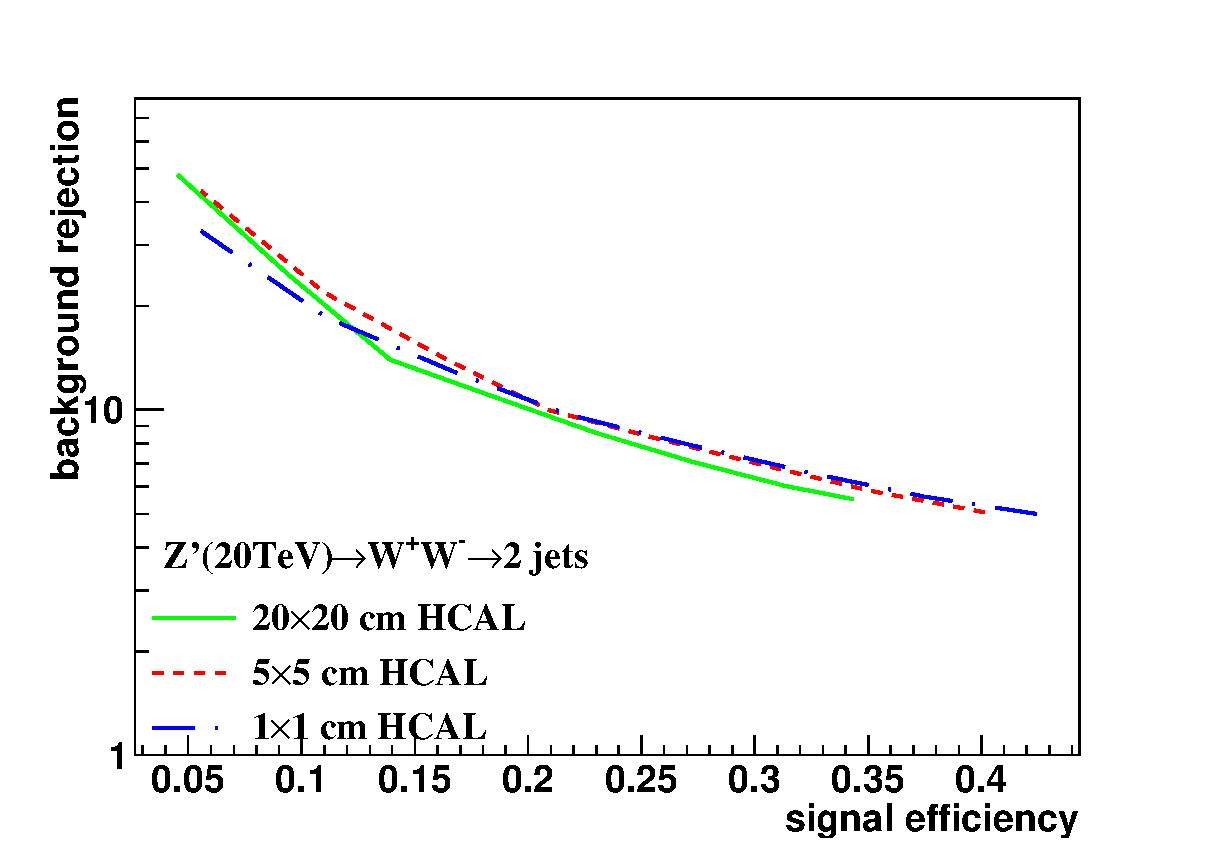
\includegraphics[width=0.43\textwidth]{figs/A_Cluster_mass_sdb2_20tev_eff_1_central_fix_ww_qq_log_no_UOF.eps}
 }
 \subfigure[Central at Median($20\times20$=,$5\times5$=,$1\times1$=) change width in cluster at 40TeV] {
 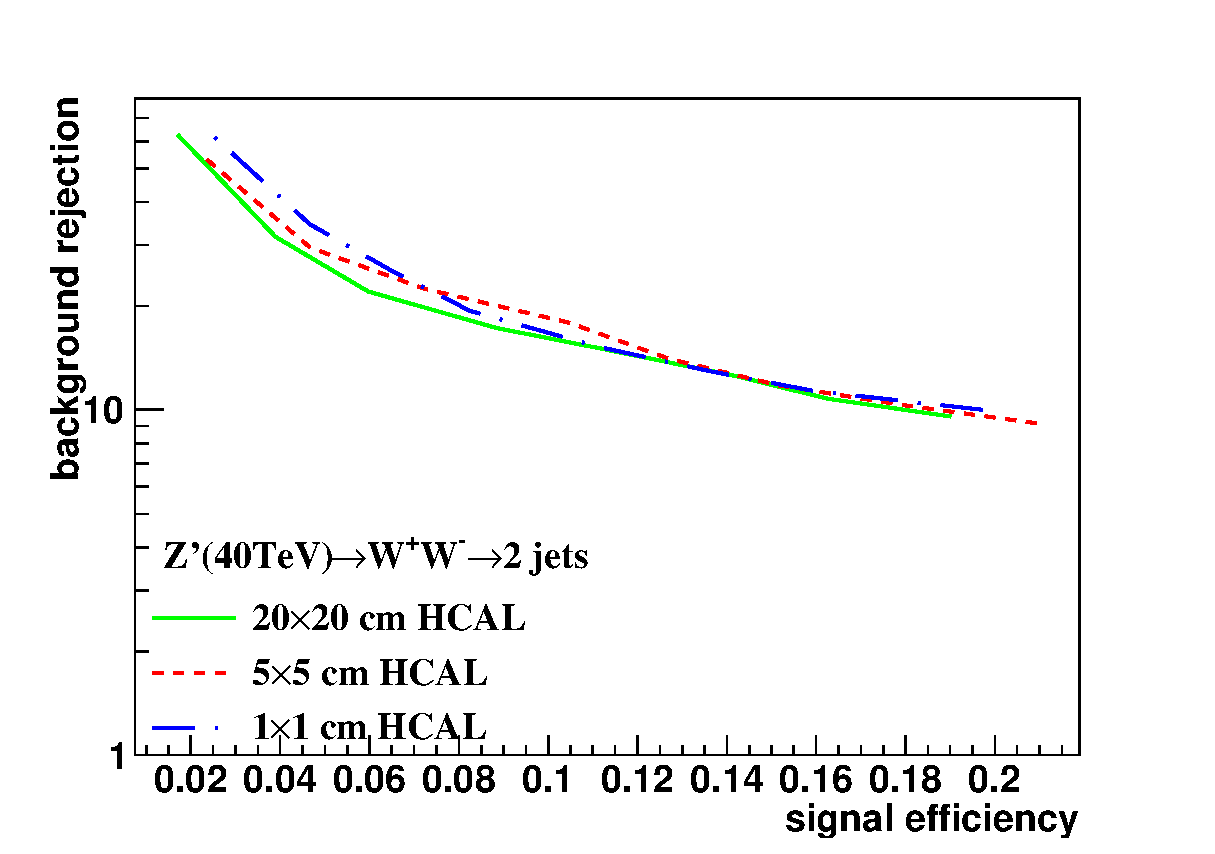
\includegraphics[width=0.43\textwidth]{figs/A_Cluster_mass_sdb2_40tev_eff_1_central_fix_ww_qq_log_no_UOF.eps}
 }
\end{center}
\caption{study of "fix central and change width" in mass soft drop at $\beta$=2, signal=ww, in 5, 10, 20, 40TeV energy of collision  in different detector sizes. Cell Size in 20$\times$20, 5$\times$5, and 1$\times$1(cm$\times$cm) are shown in each picture.}
\label{fig:cluster_tau21_tau32}
\end{figure}


\begin{figure}
\begin{center}
   \subfigure[5TeV at 20$\times$20(cm$\times$cm) in cluster] {
   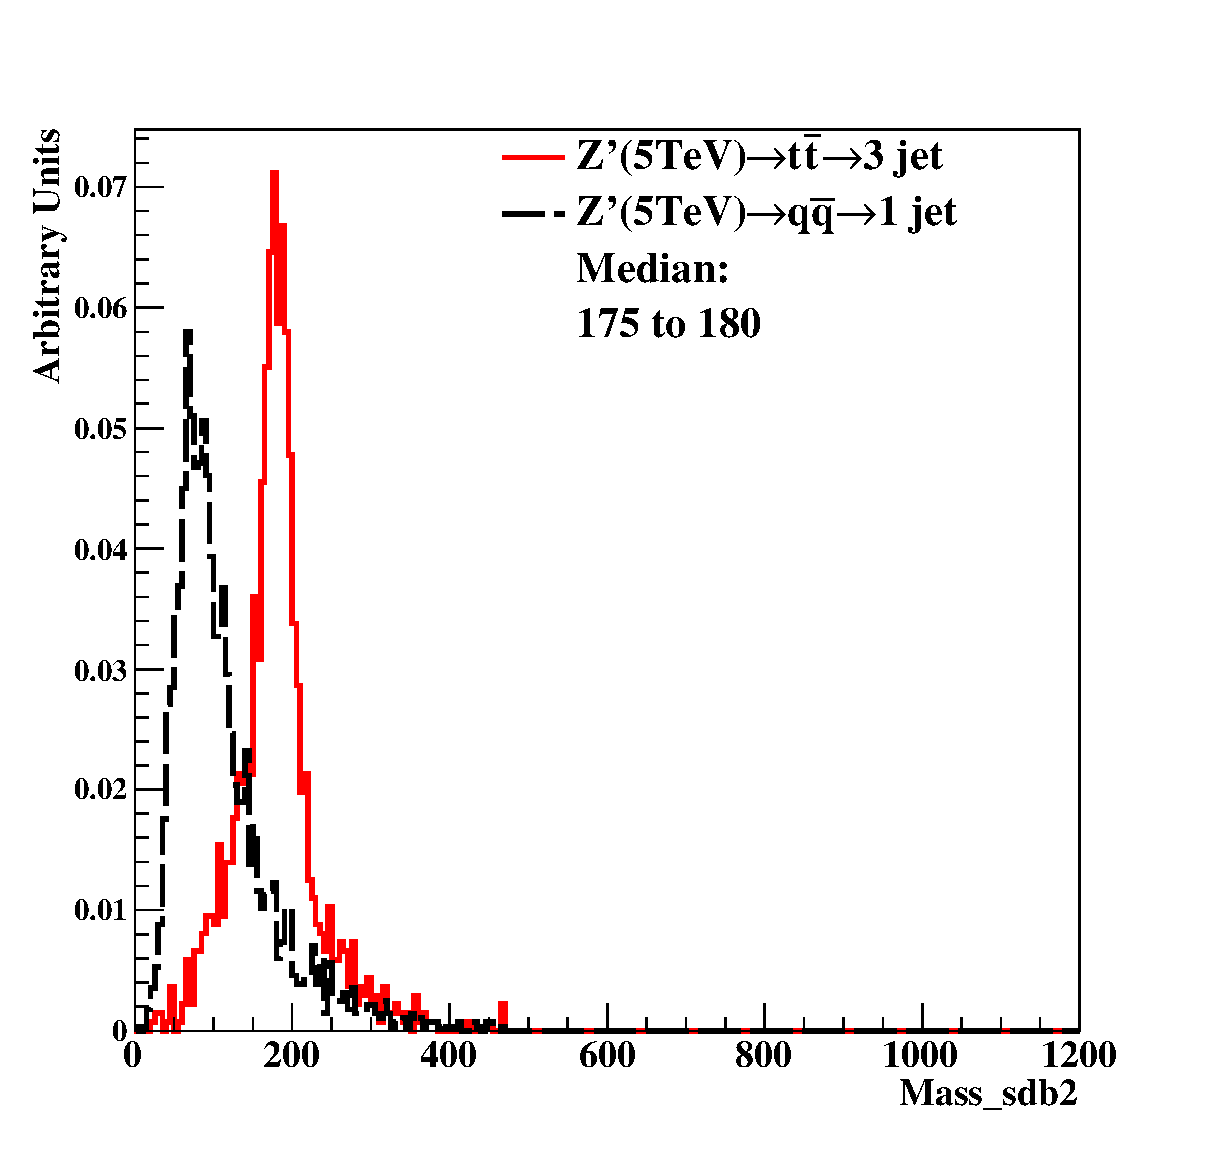
\includegraphics[width=0.22\textwidth]{figs/Dis_cluster_012_mass_sdb2_tt_5tev_04_tt_1200_no_UOF.eps}
   }
      \subfigure[10TeV at 20$\times$20(cm$\times$cm) in cluster] {
   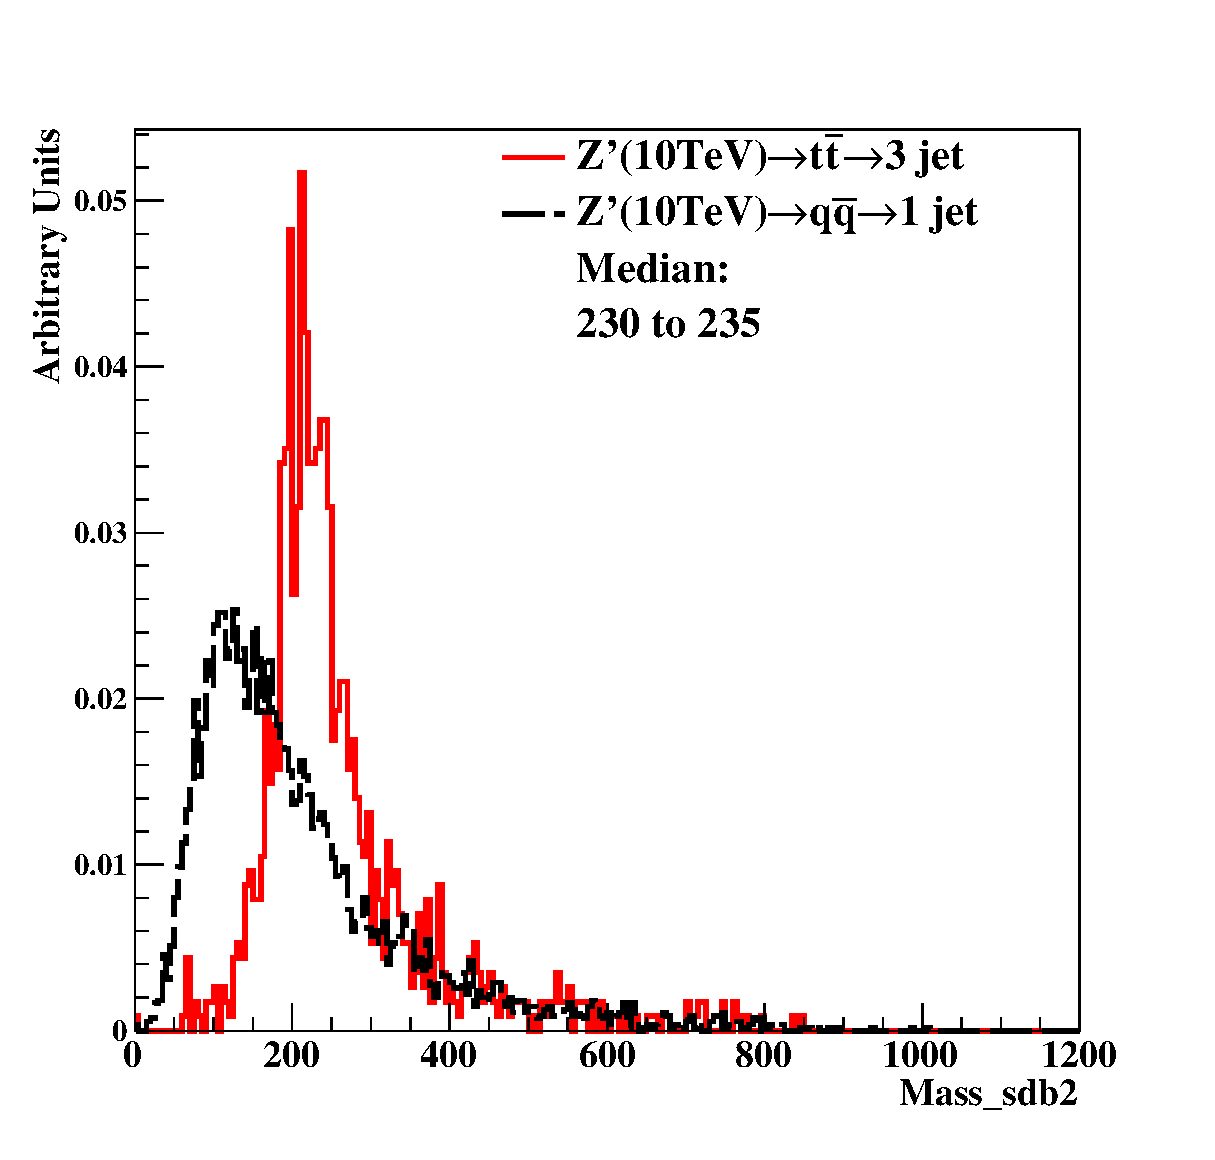
\includegraphics[width=0.22\textwidth]{figs/Dis_cluster_010_mass_sdb2_tt_10tev_04_tt_1200_no_UOF.eps}
   }
   \subfigure[20TeV at 20$\times$20(cm$\times$cm) in cluster] {
   \includegraphics[width=0.22\textwidth]{figs/Dis_cluster_010_mass_sdb2_tt_20tev_04_tt_2400_no_UOF.eps}
   }
    \subfigure[40TeV at 20$\times$20(cm$\times$cm) in cluster] {
   \includegraphics[width=0.22\textwidth]{figs/Dis_cluster_010_mass_sdb2_tt_40tev_04_tt_2400_no_UOF.eps}
   }
   \subfigure[5TeV at 5$\times$5(cm$\times$cm) in cluster] {
   \includegraphics[width=0.22\textwidth]{figs/Dis_cluster_009_mass_sdb2_tt_5tev_04_tt_1200_no_UOF.eps}
   }
   \subfigure[10TeV at 5$\times$5(cm$\times$cm) in cluster] {
   \includegraphics[width=0.22\textwidth]{figs/Dis_cluster_009_mass_sdb2_tt_10tev_04_tt_1200_no_UOF.eps}
   }
   \subfigure[20TeV at 5$\times$5(cm$\times$cm) in cluster] {
   \includegraphics[width=0.22\textwidth]{figs/Dis_cluster_009_mass_sdb2_tt_20tev_04_tt_2400_no_UOF.eps}\hfill
   }
      \subfigure[40TeV at 5$\times$5(cm$\times$cm) in cluster] {
   \includegraphics[width=0.22\textwidth]{figs/Dis_cluster_009_mass_sdb2_tt_40tev_04_tt_2400_no_UOF.eps}\hfill
   }
   \subfigure[5TeV at 1$\times$1(cm$\times$cm) in cluster] {
   \includegraphics[width=0.22\textwidth]{figs/Dis_cluster_012_mass_sdb2_tt_5tev_04_tt_1200_no_UOF.eps}\hfill
   }
    \subfigure[10TeV at 1$\times$1(cm$\times$cm) in cluster] {
   \includegraphics[width=0.22\textwidth]{figs/Dis_cluster_012_mass_sdb2_tt_10tev_04_tt_1200_no_UOF.eps}
   }
   \subfigure[20TeV at 1$\times$1(cm$\times$cm) in cluster] {
   \includegraphics[width=0.22\textwidth]{figs/Dis_cluster_012_mass_sdb2_tt_20tev_04_tt_2400_no_UOF.eps}\hfill
   }
      \subfigure[40TeV at 1$\times$1(cm$\times$cm) in cluster] {
   \includegraphics[width=0.22\textwidth]{figs/Dis_cluster_012_mass_sdb2_tt_40tev_04_tt_2400_no_UOF.eps}
   }
\end{center}
\caption{Distributions of mass soft drop at $\beta$=2, signal=tt, in 5,10TeV energy of collision  in different detector sizes. Cell Size in 20$\times$20, 5$\times$5, and 1$\times$1(cm$\times$cm) are shown here.}
\label{fig:cluster_tau21_tau32}
\end{figure}


\begin{figure}
\begin{center}
  \subfigure[Central at Median($20\times20$=,$5\times5$=,$1\times1$=) change width in cluster at 5TeV] {
  \includegraphics[width=0.43\textwidth]{figs/A_Cluster_mass_sdb2_5tev_eff_1_central_fix_tt_qq_log_no_UOF.eps}
  }
  \subfigure[Central at Median($20\times20$=,$5\times5$=,$1\times1$=) change width in cluster at 10TeV] {
  \includegraphics[width=0.43\textwidth]{figs/A_Cluster_mass_sdb2_10tev_eff_1_central_fix_tt_qq_log_no_UOF.eps}
  }
 \subfigure[Central at Median($20\times20$=,$5\times5$=,$1\times1$=) change width in cluster at 20TeV] {
 \includegraphics[width=0.43\textwidth]{figs/A_Cluster_mass_sdb2_20tev_eff_1_central_fix_tt_qq_log_no_UOF.eps}
 }
 \subfigure[Central at Median($20\times20$=,$5\times5$=,$1\times1$=) change width in cluster at 40TeV] {
 \includegraphics[width=0.43\textwidth]{figs/A_Cluster_mass_sdb2_40tev_eff_1_central_fix_tt_qq_log_no_UOF.eps}
 }
\end{center}
\caption{study of "fix central and change width" in mass soft drop at $\beta$=2, signal=tt, in 5, 10, 20, 40TeV energy of collision  in different detector sizes. Cell Size in 20$\times$20, 5$\times$5, and 1$\times$1(cm$\times$cm) are shown in each picture.}
\label{fig:cluster_tau21_tau32}
\end{figure}






